\documentclass[11pt, a4paper]{article}
%\usepackage{proj1}
\usepackage{natbib}
\usepackage{fancyhdr}  
\usepackage{subcaption}
\usepackage{caption}
\usepackage{graphicx}
\usepackage{numprint}
\usepackage{multirow}
\linespread{1.25} 
\setlength{\parindent}{0cm}
\graphicspath{{Images/}}
\usepackage{hyperref}
\usepackage{amsmath}
\usepackage{amsfonts}
\usepackage{amssymb}
\usepackage{amsthm}
\usepackage{mathtools}
\usepackage{commath}
\usepackage{bbm}

%\usepackage[sc,osf]{mathpazo}
\usepackage{subcaption}
\usepackage[a4paper, top=1in, left=1.0in, right=1.0in, bottom=1in, includehead, includefoot]{geometry} %Usually have top as 1in

\usepackage{listings}
\usepackage{color} %red, green, blue, yellow, cyan, magenta, black, white
\definecolor{mygreen}{RGB}{28,172,0} % color values Red, Green, Blue
\definecolor{mylilas}{RGB}{170,55,241}


\hypersetup{colorlinks,linkcolor={black},citecolor={blue},urlcolor={black}}
\usepackage{color}
\urlstyle{same}


\theoremstyle{definition}
\newtheorem{definition}{Definition}[section]

\newcommand{\adja}{q_a}
\newcommand{\adjb}{q_b}
\newcommand{\adjaB}{q_{a,\partial \Omega}}
\newcommand{\adjbB}{q_{b,\partial \Omega}}
\newcommand{\adjB}{q_{\partial \Omega}}
\newcommand{\Adja}{\mathbf{p}}
\newcommand{\Adjb}{q}
\newcommand{\adj}{q}
\newcommand{\Adjc}{{q}_{\partial \Omega}}
\newcommand{\ra}{\rho_a}
\newcommand{\rb}{\rho_b}
\newcommand{\w}{\mathbf{w}}
\newcommand{\f}{\mathbf{f}}
\newcommand{\ve}{\mathbf{v}}
\newcommand{\n}{\mathbf{n}}
\newcommand{\h}{\mathbf{h}}
\newcommand{\K}{\mathbf{K}}
\newcommand{\hr}{\widehat \rho}



\title{{\huge PDE-Constrained Optimization \\for Multiscale Particle Dynamics} \\ with Industrial Applications}
\author{Jonna C. Roden\\ \\Supervision by Dr Ben Goddard and Dr John Pearson\\ \vspace{0.5cm} Maxwell Institute Graduate School for Analysis and its Applications}
\date{\today}


\pagenumbering{gobble}
\begin{document}
	\maketitle
\begin{abstract}
+ Later +
	
\end{abstract}

\newpage
%\section*{Acknowledgements}
%+ Later +
%\newpage
\pagenumbering{Roman} 
\tableofcontents
%\newpage
%\listoffigures
%\listoftables
\newpage
\pagenumbering{arabic} 

\section*{Thesis Draft}	
	
\section{Introduction}
PDE-constrained optimization and multiscale particle dynamics are both fields of growing interest to academia and industry. Applying methods of PDE-constrained optimization to industrial processes is a highly relevant topic, for example in the oil and gas industry \cite{Brandman2018}, the beer industry \cite{RamirezW.F.2007Obf} and the wine industry \cite{MergerJuri2017Ocoa}. 
There are two industrial partners affiliated with this project. WEST brewery is interested in optimizing the yeast sedimentation in the beer brewing process. The company ufraction8 works on cell separation and nano filtration devices, which separate particles based on their sizes. They are interested in optimizing this process.
\\
\\
Many processes, including these two examples, can be described as interacting particle systems, using Density Functional Theory (DFT). Further examples include processes in biology and nanotechnology \cite{FrinkDFT}, as well as in chemical engineering \cite{WuJianzhong2006Dftf}.
Therefore, developing a numerical framework for PDE-constrained optimization problems, where the PDE constraint describes particle dynamics, is highly relevant. This task is challenging, because the PDEs involved are non-local, nonlinear integro-PDEs. This makes the application of standard methods, such as finite element methods, hard. Pseudospectral methods can be used to tackle the numerical challenges, such as non-local boundary conditions and dense matrices in the discretized problem.
In this report, steps towards developing this numerical method are taken by deriving a method for one- and two-dimensional test problems, which can be extended to the full problem, including the PDE describing the particle dynamics.
\\
\\
The report is structured as follows. In the next section, the PDE for the particle dynamics is derived from the Smoluchowski equation. In the third section, the PDE-constrained optimization framework is set up and first-order optimality conditions are derived for two different test problems, one diffusion type problem and one problem including an integral particle interaction term.
In the fourth section, some exact solutions and the numerical methods are introduced, such as pseudospectral methods and the multiple shooting method.
In the fifth section, some numerical experiments are presented for both introduced test problems in one and two dimensions.
In the final section, some conclusions are drawn and opportunities for future work are pointed out.


\section{Literature Review on Mean Field Optimal Control}
While mean-field games were first introduced by Lasry and Lions, \cite{LASRY2006619}, \cite{LASRY2006679},\cite{LASRY4} and \cite{Lasry2007}, and independently by Huang, Caines and Malham\'e,  \cite{Huang1}, under the name Nash certainty equivalence, the optimal control side of this class of problems is quite a new area of research. The main difficulty is a non-linear, non-local particle interaction term. Therefore, standard results in optimal control theory cannot readily be applied, and new approaches have to be developed to address theoretical and numerical challenges.
\\
\\
There are two types of models that recent work has focussed on. The most popular model is a deterministic microscopic model, which is a generalization of the well-known Cucker-Smale model, see \cite{CuckerSmale1}, \cite{CuckerSmale2}. In the mean-field limit, a Vlasov-type PDE arises. For control problems involving this class of models, the work by Fornasier et al. provides a range of theoretical results on the convergence of the microscopic optimal control problem to a corresponding macroscopic problem, using methods of optimal transport and a $\Gamma$-limit argument, proving existence of optimal controls in the mean-field setting, see \cite{Fornasier_2014},
\cite{Fornasier_2014no2}
and \cite{fornasier_lisini_orrieri_savare_2019}. The work focusses on sparse control strategies, where one or more agents influence a larger crowd.
Additional work on sparse control strategies can be found in \cite{piccoli2014no1}, as well as in the review paper \cite{Fornasier_20161no1}.
In \cite{burger2019meanfield}, an alternative method, an $L_2$ calculus, is developed, and convergence results are proved. The control in this work is applied through external agents. 
\\
Numerical advances have been made in \cite{burger2019instantaneous} and \cite{burger2016controlling}, where sparse and other control strategies through the external agents are considered. In both papers a Strang-Splitting scheme, \cite{ChengC.Z1976Tiot}, is applied to solve the optimal control problem. The numerical results verify the convergence of the microscopic control problem to its mean-field limit.
Furthermore, in \cite{albi2016selective}, different selective control strategies are considered, and an iterative numerical method is chosen, where the interaction term is approximated stochastically.
\\
\\
Fewer work has been done on the optimal control of the Fokker-Planck PDE, which arises as the mean-field limit of a stochastic microscopic model. Some theoretical results on this model are published. In \cite{albi2016mean}, the existence of optimal controls for microscopic and macroscopic versions of a class of problems is proved and a rigorous derivation of first-order optimality conditions is given. 
Following this, \cite{carrillo2019mean} discusses the existence and regularity of an optimal control problem of this type on periodic domains, including the well-posedness of the Fokker-Planck equation. In \cite{Pinnau_2017} and  \cite{carrillo2018no1}, the convergence of the microscopic optimal control problem to its mean-field limit is proved.
Numerical results on the model include those presented in \cite{Pinnau_2017}, where a Strang-Splitting scheme, \cite{gilbertstrang1}, is applied, and in which convergence to the mean field optimal control problem is shown numerically. Furthermore, in \cite{albi2016mean}, an optimal control hierarchy, including instantaneous and Boltzmann-type controls, is proposed. The mean-field first-order optimality system in \cite{albi2016mean} is solved using a Chang-Cooper scheme for the forward equation, finite differences for the adjoint equation, while approximating the integrals using a Monte-Carlo scheme. This is coupled by a sweeping algorithm, where updates are made through the gradient equation.
Some numerical results on a porous media version of the Fokker-Planck equation are presented in \cite{carrillo2018no1}. In \cite{Albi_2014no1} and \cite{albi2014kinetic}, steady state solutions to a Fokker-Planck-type PDE are considered, however, the main focus  are Boltzmann-type approaches to solving the optimal control problem.
\\
\\
The most common control types in the literature are flow control, e.g. \cite{albi2016mean}, control through the interaction term, e.g. \cite{Fornasier_2014no2}, as well as control through external agents, e.g. \cite{burger2016controlling}. 
Most papers do not consider boundary conditions, because it is assumed that the particle distribution is of compact support, see \cite{fornasier_lisini_orrieri_savare_2019}, \cite{burger2019meanfield}, or \cite{burger2016controlling}. No-flux boundary conditions, which are of high relevance in applications, are not often found in the literature, but are considered in \cite{albi2016mean} and \cite{carrillo2018no1}.
Our work considers the mean-field equation of Fokker-Planck type, flow-type control or control through a source term and no-flux or Dirichlet boundary conditions, in order to address a broad range of test problems and real world applications. 
\\
\\
As described above, some numerical methods have been developed for solving optimal control problems involving non-local, non-linear PDEs. Most of these papers however focus on other methods and use the mean-field optimal control as verification tool, see \cite{albi2016mean}, \cite{Pinnau_2017}. It takes large computational effort to solve these problems, which increases with dimensionality, see \cite{burger2019instantaneous}, \cite{burger2016controlling}. 
We are proposing a new numerical framework for PDE-constrained optimization applied to multiscale particle dynamics, where a fixed point algorithm is implemented to solve the first-order optimality system. This update scheme is inspired by the sweeping algorithm in \cite{albi2016mean}, and similar to the gradient descent method in \cite{Burger1}. The algorithm is coupled with pseudospectral methods, used to discretize space and time domains. This composition of methods offers an efficient and accurate solver for the class of problems discussed. To our knowledge, it is the first time that pseudospectral methods are used in the context of optimal control problems.


\section{Multiscale Particle Dynamics}


The aim of this section is to model the dynamics of particles, which are suspended in a bath. The particles evolve in time and in some domain $\Omega$ in space. Instead of modelling the movement of a particular particle, a space coordinate $r \in \Omega$ is fixed. The probability of a particle being at the position $r$ at time $t$ is modelled as a  distribution $\rho(r,t)$, the one-body particle density.
The model equations are:
\begin{align}\label{sysParticleModel1}
\partial_t \rho(r,t) &= \nabla \cdot \bigg(\big(\nabla  + \nabla V_{ext} + \int_\Omega \rho(r') \nabla V_2(|r-r'|)dr' - \mathbf{w} \big) \rho(r,t) \bigg),\\
&:=\nabla \cdot \mathbf{j},\notag \\
\notag  \\
\mathbf{j} \cdot \mathbf{n}&=0 \quad  \ \text{on   } \quad  \partial \Omega, \notag  \\
\rho(0) &=\rho_0 \quad \text{at} \quad t=t_0, \notag 
\end{align}
where $\mathbf{j}=\big(\nabla  + \nabla V_{ext} + \int_\Omega \rho(r') \nabla V_2(|r-r'|)dr' - \mathbf{w} \big) \rho(r,t) $ and $\mathbf{n}$ denotes the outward normal to $\partial \Omega$, compare to \cite{RexLoewen1}.
 The equation describes the particle dynamics, including a time derivative, a diffusion term, and an external potential $V_{ext}$, whose negative gradient is a body force such as gravity. Furthermore, there is a term describing the background flow field of the bath, $\mathbf{w}$, and a particle interaction term.\\
 This particle interaction term describes the interactions of two particles at the position $r$ and some other position $r' \in \Omega$, where $r' \neq r$. The forces between the particles at $r$ and  $r'$ are represented by $-\nabla V_2(|r-r'|)$. This is multiplied by the particle density at $r'$, $\rho(r')$, and the particle density at $r$, $\rho(r)$. Since each position $r' \in \Omega$ needs to be considered, the resulting expression is integrated over all $r'$.\\
The particle interaction in (\ref{sysParticleModel1}) is restricted to two-body interactions and can be extended to three- or more body interaction terms, which makes the model equations more accurate and complex. The inclusion of higher-order terms is dependent on the application. Furthermore, the forces between the particles included here only describe interactions such as attraction and repulsion. The model neglects hydrodynamic interactions, which are the effects of the particles moving in the bath. This movement causes a change in the flow field, which in turn influences the surrounding particles. This is a non-local phenomenon, which is more complex to model, however, significant to include in various applications. 

\subsection{Deriving Model Equations}
The model equation (\ref{sysParticleModel1}) can be derived from the full $N$-body particle distribution. This has been done by M. Rex and H. Loewen \cite{RexLoewen1}, whose derivation is followed in this section.	
On the microscopic level, a probability distribution $P(r^N,t)$ of the total number $N$ particles in the bath at time $t$ is considered, where $r^N= (r_1, r_2,...,r_N)$, and $r_i \in \mathbf{R}^3$, $i=1,2,...,N$. 
The dynamics of the probability distribution $P(r^N,t)$ can be described by the Smoluchowski equation, as presented in \cite{RexLoewen1}:
\begin{align} \label{eqnPpde}
\partial_t P(r^N,t)= \sum_{i,j}^N \nabla_i \cdot \bigg( D_{i,j}(r^N) \bigg( \nabla_j + \frac{\nabla_j U(r^N,t)}{k_BT} - \mathbf{w}(r_i) \bigg) P(r^N,t) \bigg),
\end{align}
where $\nabla_i$ refers to the operation with respect to the coordinate $r_i$. The term $D_{i,j}(r^N)$ is the diffusion tensor, which describes the hydrodynamic interactions of the particles at $r_i$ and $r_j$, $U(r^N,t)$ is a potential, which could include an external potential and particle interactions, $T$ is the temperature, and $k_B$ is the Boltzmann constant. A background flow is defined by $\mathbf{w} \in \mathbf{R}^3$, describing the flow of the bath fluid.
 Note that this version of the equation is more general than the representation in the paper, due to the extra term $\mathbf{w}$. The aim is to derive a three dimensional approximation $\rho^{(1)}(r_1,t)$ to (\ref{eqnPpde}). The following $n$-body densities are defined as in \cite{RexLoewen1}:
\begin{align*}
\rho^{(1)}(r_1,t) &= N \int_\Omega dr_2.... dr_N P(r^N,t):= \rho(r,t),\\
\vdots\\
\rho^{(n)}(r_n,t) &= \frac{N!}{(N-i)!} \int_\Omega dr_{n+1}.... dr_N P(r^N,t),
\end{align*} 
where $\Omega=\mathbf{R}^{3N}$.
The $n$-body densities are derived by integrating the full $N$ particle probability distribution over $r_{n+1},...r_N$, and multiplying it by a prefactor. This definition is chosen to suit the computations, which are detailed below.
In order to derive a three-dimensional approximation in terms of the one-body density $\rho(r,t)$, initially a simplification of (\ref{eqnPpde}) is considered and then extended in later sections to derive the approximation for the full system. 

\subsubsection{The Diffusion Equation}
Considering $D_{i,j}=\delta_{i,j}$, $U=0$ and $\mathbf{w}=0$ in (\ref{eqnPpde}), the diffusion equation is recovered:
\begin{align*} 
\partial_t P(r^N,t) &= \sum_{i}^N \nabla_i \cdot \bigg(\nabla_i   P(r^N,t) \bigg)= \sum_{i}^N \Delta_i P(r^N,t)\\
&= \Delta_{r^N} P(r^N,t),
\end{align*}
where $\sum_{i}^N \Delta_i := \Delta_{r^N}$.

In order to derive the one-body density $\rho(r,t)$ for the diffusion equation, the equation is multiplied by $N$ and integrated over all other positions $r_2,...,r_N$:
\begin{align*} 
\int_\Omega N \partial_t P(r^N,t)dr_2...dr_N &= \int_\Omega N \sum_{i}^N \nabla_i \cdot \bigg(\nabla_i   P(r^N,t) \bigg)dr_2...dr_N.
\end{align*}
The integration is only dependent on space, not on time, so that the time derivative can be taken out of the integral. Furthermore, the sum on the right-hand side of the equation, as well as the integration, is finite. Therefore, Fubini's Theorem can be used to take the sum out of the integral. The equation is then:
\begin{align*} 
N \partial_t \int_\Omega P(r^N,t)dr_2...dr_N &=N \sum_{i}^N \int_\Omega  \nabla_i \cdot \bigg(\nabla_i   P(r^N,t) \bigg)dr_2...dr_N.
\end{align*}
The Divergence Theorem can be applied to $i=2,...,N$, while for $i=1$ the integral remains unchanged, since the integration is independent of $r_1$. The equation is now:
\begin{align*} 
N \partial_t \int_\Omega P(r^N,t)dr_2...dr_N &=N \sum_{i=2}^N \int_{\partial \Omega} \frac{\partial P(r^N,t)}{\partial n} dr_2...dr_N + N\int_\Omega \nabla_1 \cdot \bigg(\nabla_1   P(r^N,t) \bigg)dr_2...dr_N,\\
\end{align*}
where $n$ is the outward normal. 
Now, the boundary condition for $P(r^N,t)$ can be employed. Since $P$ is a probability distribution over a finite number of positions $r_i$, on an infinite domain $\Omega= \mathbf{R}^{3N}$, the natural boundary condition is that $P$ and its derivatives vanish on the boundary $\partial \Omega$, i.e. at infinity.
Furthermore, considering the fact that $\nabla_1$ is constant with respect to the integration variables, it can be taken out of the integral and the following result is found, where the definition $\rho(r,t)= N \int_\Omega P(r^N,t)dr_2...dr_N$ is used:
\begin{align*} 
\partial_t \rho(r,t) &= \nabla_1 \cdot \bigg(\nabla_1 N \int_\Omega  P(r^N,t) \bigg)dr_2...dr_N,\\
&=  \nabla_1 \cdot(\nabla_1  \rho(r,t) ).
\end{align*}
This is a one-body diffusion equation in $\mathbf{R}^3$, which is an approximation to the diffusion equation of the full $N$ particle probability distribution $P(r^N,t)$. In a last step, the subscript of $\nabla_1$ can be dropped, since the only position considered in this equation is $r_1$. The final equation is
\begin{align} \label{eqnPMDiffTerm}
\partial_t \rho(r,t) &=  \nabla \cdot(\nabla \rho(r,t) ).
\end{align}


\subsubsection{Adding Pairwise Interactions}
After deriving the one-body equation for the diffusion term, a more complex version of (\ref{eqnPpde}) can be considered. Let $D_{i,i}= \delta_{i,j}$, as before, but define $U$ as: 
\begin{align*}
U= \sum_{m=1}^N V_{ext}(r_m,t) + \frac{1}{2} \sum_{m \neq n}^N V_2(|r_m - r_n|),
\end{align*}
where $V_{ext}$ is an external potential and $V_2$ is the potential due to forces between two particles.
The PDE considered is again a simplified version of (\ref{eqnPpde}) and has the form:
\begin{align} \label{eqnPpde2}
 \partial_t P(r^N,t)= \sum_{i}^N \nabla_i \cdot \bigg(\bigg( \nabla_i + \nabla_i \bigg( \sum_{m=1}^N V_{ext}(r_m,t) + \frac{1}{2} \sum_{m \neq n}^N V_2(|r_m - r_n|)\bigg)  \bigg) P(r^N,t) \bigg),
 \end{align}
where $k_B T=1$ for simplicity.
The diffusion term in the equation can be treated equivalently to the procedure in the previous section.
The two new terms are treated similarly. The equation is multiplied by $N$ and integrated over $r_2...r_N$.
This gives:
\begin{align*} 
&N\int_\Omega \partial_t P(r^N,t) dr_2...dr_N\\
=& N\int_\Omega \sum_{i}^N \nabla_i \cdot \bigg(\bigg( \nabla_i + \nabla_i \bigg( \sum_{m=1}^N V_{ext}(r_m,t) + \frac{1}{2} \sum_{m \neq n}^N V_2(|r_m - r_n|)\bigg)  \bigg) P(r^N,t) \bigg) dr_2...dr_N,\\
=& N\int_\Omega \sum_{i}^N \nabla_i \cdot \nabla_i P(r^N,t)dr_2...dr_N + N\int_\Omega \sum_{i}^N \nabla_i \cdot \bigg( P(r^N,t) \nabla_i \sum_{m=1}^N V_{ext}(r_m,t) \bigg) dr_2...dr_N\\ +& N\int_\Omega \sum_{i}^N \nabla_i \cdot \bigg( P(r^N,t)\nabla_i \frac{1}{2} \sum_{m \neq n}^N V_2(|r_m - r_n|) \bigg) dr_2...dr_N\\
:=& I_1 + I_2 +I_3.
\end{align*}
The left-hand side satisfies $N\int_\Omega \partial_t P(r^N,t) dr_2...dr_N= \partial_t \rho(r,t)$ from the previous section.
The integral $I_1$, by (\ref{eqnPMDiffTerm}), satisfies:
\begin{align} \label{eqnPInt1}
I_1=  N\int_\Omega \sum_{i}^N \nabla_i \cdot \nabla_i P(r^N,t)dr_2...dr_N = \Delta \rho(r,t).
\end{align}
Next, the integral $I_2$ is considered:
\begin{align*}
I_2&=N\int_\Omega \sum_{i}^N \nabla_i \cdot \bigg( P(r^N,t) \nabla_i \sum_{m=1}^N V_{ext}(r_m,t) \bigg) dr_2...dr_N. 
\end{align*}
By the same argument as in the previous section, the integration and summation can be swapped. Furthermore, $\nabla_i \sum_{m=1}^N V_{ext}(r_m,t) =\nabla_i V_{ext}(r_i,t)$, since all other terms in the sum are zero, when $\nabla_i$ is applied to a term independent of $r_i$. The resulting equation is:
\begin{align*}
I_2&=N\sum_{i}^N\int_\Omega  \nabla_i \cdot \bigg( P(r^N,t) \nabla_i V_{ext}(r_i,t) \bigg) dr_2...dr_N. 
\end{align*}
As before, the Divergence Theorem can be used for all variables $r_2,...r_N$, while the equation for $r_1$ remains unchanged. This gives:
\begin{align*}
I_2&=N\sum_{i=2 }^N\int_{ \partial \Omega}  P(r^N,t) \frac{\partial V_{ext}(r_i,t)}{\partial {n}}  dr_2...dr_N + N\int_\Omega  \nabla_1 \cdot \bigg( P(r^N,t) \nabla_1 V_{ext}(r_i,t) \bigg) dr_2...dr_N, 
\end{align*}
where ${n}$ is again the outward normal.
Then, applying the boundary conditions for $P(r^N,t)$, as discussed above, and realising that $\nabla_1 V_{ext}(r_i,t)=\nabla_1 V_{ext}(r_1,t)$, since this expression is zero for all $r_i \neq r_1$, the following equations is derived:
\begin{align*}
I_2&= N \int_\Omega  \nabla_1 \cdot \bigg( P(r^N,t) \nabla_1 V_{ext}(r_1,t) \bigg) dr_2...dr_N. 
\end{align*}
Since $r_1$ is constant with respect to the integration variables, all terms only depending on $r_1$ can be taken out of the integral to give:
\begin{align*}
I_2&= N \nabla_1 \cdot \bigg(\nabla_1 V_{ext}(r_1,t)\int_\Omega  P(r^N,t) dr_2...dr_N\bigg)\\
&=   \nabla_1 \cdot \bigg( (\nabla_1 V_{ext}(r_1,t)) \rho(r,t)\bigg).
\end{align*}
Then, dropping the subscripts, $I_2$ is:
\begin{align}\label{eqnPInt2}
I_2= \nabla \cdot \bigg( \rho(r,t)\nabla V_{ext}(r_1,t) \bigg).
\end{align}

The final term in the PDE that has to be considered is $I_3$:
\begin{align*}
I_3 = N\int_\Omega \sum_{i}^N \nabla_i \cdot \bigg( P(r^N,t)\nabla_i \frac{1}{2} \sum_{m \neq n}^N V_2(|r_m - r_n|) \bigg) dr_2...dr_N.
\end{align*}
As for $I_1$ and $I_2$, the integration and summation operations can be swapped, and the Divergence Theorem can be applied to $r_2,...r_N$ to give:
\begin{align*}
I_3 =& \frac{1}{2}N \sum_{i}^N \int_\Omega  \nabla_i \cdot \bigg( P(r^N,t) \nabla_i \sum_{m \neq n}^N V_2(|r_m - r_n|) \bigg) dr_2...dr_N\\
=&\frac{1}{2}N\int_{\partial \Omega} \sum_{i=2}^N  \bigg( P(r^N,t) \sum_{m \neq n}^N \frac{ \partial V_2(|r_m - r_n|)}{\partial n} \bigg) dr_2...dr_N\\
 +& \frac{1}{2}N\int_\Omega  \nabla_1 \cdot \bigg( P(r^N,t)\nabla_1 \sum_{m \neq n}^N  V_2(|r_m - r_n|) \bigg) dr_2...dr_N.
\end{align*}
The boundary conditions for $P$ are applied to set the first term to zero. \\
The term $\nabla_1 \sum_{m \neq n}^N  V_2(|r_m - r_n|)$ has to be examined in more detail. Since the gradient is applied with respect to $r_1$, one of the $r_m,r_n$ in the double sum has to be $r_1$, since all other terms will be zero when the gradient is applied.
Therefore:
\begin{align*}
\nabla_1 \sum_{m \neq n}^N  V_2(|r_m - r_n|)=\nabla_1 \sum_{n=2}^N  V_2(|r_1 - r_n|) + \nabla_1 \sum_{m=2}^N  V_2(|r_m - r_1|).
\end{align*}
 Since $m$ and $n$ are dummy variables and  $|r_m - r_n|=|r_n - r_m|$ is symmetric, the previous equation reduces to:
 \begin{align*}
 \nabla_1 \sum_{m \neq n}^N  V_2(|r_m - r_n|)=2 \nabla_1 \sum_{n=2}^N  V_2(|r_1 - r_n|) .
 \end{align*} 
Then $I_3$ becomes:
\begin{align*}
I_3 
=& N\int_\Omega  \nabla_1 \cdot \bigg( P(r^N,t)\nabla_1 \sum_{n=2}^N  V_2(|r_1 - r_n|) \bigg) dr_2...dr_N.
\end{align*}
Writing out the sum in $N$ explicitly gives:
\begin{align*}
I_3 
=& N\int_\Omega  \nabla_1 \cdot \bigg( P(r^N,t)\nabla_1 V_2(|r_1 - r_2|) \bigg) dr_2...dr_N\\
+& N\int_\Omega  \nabla_1 \cdot \bigg( P(r^N,t)\nabla_1 V_2(|r_1 - r_3|) \bigg) dr_2...dr_N\\
\vdots \\
+& N\int_\Omega  \nabla_1 \cdot \bigg( P(r^N,t)\nabla_1 V_2(|r_1 - r_N|) \bigg) dr_2...dr_N.
\end{align*}
Since the particles are indistinguishable, a permutation argument can be employed and the indices $r_i$ in the terms $V_2(|r_1 - r_i|)$ can be relabelled, such that $r_i=r_2$, $i=3,...,n$, for each term in the sum. Since the integration is symmetric, the integration order can be permuted arbitrarily and hence does not have to be adapted. This results in $N-1$ identical equations, and so $I_3$ is:
\begin{align*}
 I_3 
 =& N(N-1) \int_\Omega  \nabla_1 \cdot \bigg( P(r^N,t)\nabla_1 V_2(|r_1 - r_2|) \bigg) dr_2...dr_N.
\end{align*}
Considering now the definition of the $n$-body particle distributions, $I_3$ can be written in terms of the two-body distribution $\rho^{(2)}(r_1,r_2,t)= N(N-1) \int_\Omega dr_3...dr_N P(r^N,t)$. Terms that only depend on $r_1$ can be taken out of the integral. Then $I_3$ is:
\begin{align*}
I_3 
=& N(N-1)  \nabla_1 \cdot \bigg( \bigg(\nabla_1 \int_\Omega  V_2(|r_1 - r_2|) \bigg) P(r^N,t) \bigg) dr_2...dr_N.
\end{align*}
Since $V_2$ only depends on $r_2$ and the order of integration is arbitrary, the integral can be rewritten as follows:
\begin{align*}
I_3 
=&  \nabla_1 \cdot \bigg( \nabla_1 \int_\Omega  V_2(|r_1 - r_2|) \bigg(N(N-1) \int_\Omega  P(r^N,t)  dr_3...dr_N \bigg) dr_2 \bigg)\\
=&  \nabla_1 \cdot \bigg( \nabla_1 \int_\Omega  V_2(|r_1 - r_2|) \rho^{(2)}(r_1,r_2,t) dr_2 \bigg).
\end{align*}
Dropping the indices on $\nabla_1$, the equation is:
\begin{align} \label{eqnPInt3}
I_3 
=&  \nabla\cdot \bigg( \nabla \int_\Omega  V_2(|r - r_2|) \rho^{(2)}(r,r_2,t) dr_2 \bigg).
\end{align}
The full three dimensional approximation of (\ref{eqnPpde2}) is found by combining (\ref{eqnPInt1}), (\ref{eqnPInt2}) and (\ref{eqnPInt3}), to give:
\begin{align*}
\partial_t \rho(r,t) &=
 \nabla\cdot \bigg(\nabla \rho(r,t)
+ \rho(r,t)\nabla V_{ext}(r_1,t) 
+ \int_\Omega \nabla  V_2(|r - r_2|) \rho^{(2)}(r,r_2,t) dr_2 \bigg).
\end{align*}
This equation is not closed, since it depends on $\rho^{(2)}(r,r_2,t)$. 
There are different approaches to closing the equation, and two of them are discussed below.

Note that the derivation for $\mathbf{w}$ term follows the same steps as above and is therefore omitted.
\subsection{Approximating the Two-Body Density}
There are different ways to approximate the two-body density $\rho^{(2)}$. In this section, two of these are presented; the Mean Field Approximation and Density Functional Theory.
\subsubsection{The Mean Field Approximation}
In order to use a mean field approach, a modelling assumption has to be made. It is assumed that the particles in the bath are only weakly interacting and the resulting approximation is that of independence. It is assumed that the two-body density of particles $r_1$ and $r_2$ is approximately the product of the individual one-body densities of $r_1$ and $r_2$, that is:
\begin{align*}
\rho^{(2)}(r,r_2,t)\approx \rho(r_1,t)\rho(r_2,t),
\end{align*}
as in \cite{RexLoewen1}.
The resulting closed PDE is:
\begin{align}\label{eqnMeanFieldApprox1}
\partial_t \rho(r,t) &=
\nabla\cdot \bigg( \bigg(\nabla 
+ \nabla V_{ext}(r_1,t) 
+\int_\Omega  \nabla  V_2(|r - r_2|) \rho(r_2,t) dr_2 \bigg) \rho(r,t) \bigg).
\end{align}
In the context of the mean field approximation, the integral term can be interpreted as the sum of forces between a particle at a position $r$ and all other particles in $\Omega$.
However, the independence approximation is often not practical in modelling industrial phenomena and so an alternative approach needs to be considered, which includes the effects of the two-body density.
\subsubsection{The Adiabatic Approximation}
Another approach for approximating $\rho^{(2)}$ is using Density Functional Theory (DFT). DFT shows that at equilibrium, when $\partial_t \rho=0$, there exists a free energy functional $\mathcal{F}$, such that:
\begin{align*}
&\nabla \rho(r,t)
+ \rho(r,t)\nabla V_{ext}(r_1,t) 
+ \int_\Omega \nabla  V_2(|r - r_2|) \rho^{(2)}(r,r_2,t) dr_2 \\
 &= \rho(r,t) \nabla \frac{\delta \mathcal{F[\rho]}}{\delta \rho},
\end{align*}
where $\frac{\delta}{\delta \rho}$ is the functional derivative with respect to $\rho$.
While in most cases $\mathcal{F}$ is not known explicitly, it is known that at equilibrium $\nabla \frac{\delta \mathcal{F[\rho]}}{\delta \rho}=0$, and therefore it can be assumed that the PDE can be rewritten as:
\begin{align}\label{eqnAdiaAprox1}
\partial_t \rho(r,t) = \nabla \cdot \bigg( \rho(r,t) \nabla \frac{\delta \mathcal{F[\rho]}}{\delta \rho} \bigg), 
\end{align}
as discussed in \cite{GoddardPseudospectralCode1}.
This is called the Adiabatic Approximation, and $\mathcal{F}$ contains all of the information about particle correlations, if it is known.
For non-interacting particles, the explicit form for $\mathcal{F}[\rho]$ is known to be:
\begin{align}\label{eqnFhardrod}
\mathcal{F}[\rho] = \int \rho(\log(\rho)-1) dr,
\end{align}
see \cite{Tarazona2008}.

To show that $\mathcal{F}[\rho]$ satisfies the adiabatic approximation (\ref{eqnAdiaAprox1}), the functional derivative can be computed and substituted into (\ref{eqnAdiaAprox1}). 
Since $\mathcal{F}$ is of the form $\mathcal{F}[\rho] = \int f(r,\rho(r), \nabla \rho(r))dr$, where $f(r,\rho(r), \nabla \rho(r))= \rho(\log(\rho)-1)$, a function $\phi$ of compact support can be defined, as discussed in \cite{CalculusofVariations1}, such that:
\begin{align*}
\int \frac{\delta \mathcal{F}[\rho]}{\delta \rho} \phi(r) dr &= \bigg[ \frac{d}{d \epsilon} \int f(r,\rho(r) + \epsilon \phi, \nabla \rho(r) + \epsilon \nabla \phi) dr \bigg]_{\epsilon=0}\\
&= \int \bigg( \frac{\partial f}{ \partial \rho} - \bigg( \nabla \cdot \frac{\partial f}{\partial \nabla \rho} \bigg) \bigg) \phi(r) dr.
\end{align*}
Since this holds for all functions $\phi \in C_0^\infty (\Omega)$, the following holds:
\begin{align*}
\frac{\delta \mathcal{F}[\rho]}{\delta \rho} =\bigg( \frac{\partial f}{ \partial \rho} - \bigg( \nabla \cdot \frac{\partial f}{\partial \nabla \rho} \bigg) \bigg).
\end{align*}
Applying this result to (\ref{eqnFhardrod}) results in:
\begin{align*}
\frac{\delta \mathcal{F}[\rho]}{\delta \rho} &= \frac{\delta}{\delta \rho} \bigg(\int \rho(\log(\rho)-1) dr \bigg)\\
&=  \frac{\partial}{ \partial \rho}(\rho(\log(\rho)-1)) - \nabla \cdot \bigg(\frac{\partial}{\partial \nabla \rho} (\rho(\log(\rho)-1) \bigg)\\
&=  \frac{\partial}{ \partial \rho}(\rho(\log(\rho)-1))\\
&= \log \rho. 
\end{align*}
Applying the gradient to this result gives:
\begin{align*}
\nabla \frac{\delta \mathcal{F}[\rho]}{\delta \rho} = \nabla \log \rho = \frac{\nabla \rho}{\rho}.
\end{align*}
Substituting this into (\ref{eqnAdiaAprox1}) results in:
\begin{align*}
\partial_t \rho(r,t) &= \nabla \cdot \bigg( \rho(r,t) \nabla \frac{\delta \mathcal{F[\rho]}}{\delta \rho} \bigg)\\
&= \nabla \cdot \bigg( \rho(r,t)  \frac{\nabla \rho(r,t) }{\rho(r,t)}  \bigg)\\
&= \nabla \cdot \nabla \rho(r,t) \\
&= \Delta \rho(r,t).
\end{align*}
This shows that the particular choice of $\mathcal{F}$, defined by (\ref{eqnFhardrod}), recovers the diffusion equation when substituted into (\ref{eqnAdiaAprox1}). This is to be expected, since $\mathcal{F}$ represents non-interacting particles.
	

\section{PDE-Constrained Optimization} 

The aim of this project is to work towards using the particle model derived in the previous section to describe an industrial process and optimize this process with minimal cost involved.
It is of interest to achieve a particle distribution $\hat{\rho}$ in some time over some domain $\Omega$.  
In the context of PDE-constrained optimization, the aim is to minimize the distance between a state variable $\rho$ and a desired state $\hat\rho$, in some norm, while also minimizing the cost involved in reaching the desired state. This minimization is constrained by the underlying physics of the particle system. The PDE describing the particle dynamics is called the state equation.
\newline
Achieving the desired state $\hat\rho$ as close as possible can be of interest either for all times, as in this report, or only at some times, such as the final time $T$. In order to achieve $\hat \rho$, the particle distribution $\rho$ can be controlled through a so-called control variable, denoted by $u$. The control can be applied in various ways, which is dependent on the application. Since the background flow influences the particle distribution $\rho$, $\hat\rho$ can try to be reached by changing the flow field. Then the flow field is the control $u$. Alternatively, $u$ could represent the temperature or the geometry of the boundaries of the bath. Moreover, $u$ could be a parameter in the body force or in the particle interaction term, influencing the particle distribution through the forces involved. Note that $u$ cannot always influence the system enough to reach the desired state $\hat \rho$. This highly depends on the choice of $\hat \rho$, the physics of the problem and on the choice of the parameter $\beta$, which is discussed below.
Since controlling $\rho$ requires energy, $u$ can be thought of as the cost involved in reaching $\hat\rho$. 
\\ 
The weight of the control is determined by the so-called regularization parameter, $\beta$. If $\beta$ is small, the desired state will be reached, however, at a high cost. If $\beta$ is large, the control will be minimized, but the desired state might not be reached. The choice of $\beta$ depends on the application involved. It is generally of interest to find a range of $\beta$ values, for which the solution to the optimization problem is robust. 
The PDE-constrained optimization problem of interest in this report is of the form:
\begin{align} \label{sysPDEconOpti1}
&\min_{\rho,\mathbf{w}} \quad \frac{1}{2}\norm{\rho- \hat{\rho}}_{L^2}^2 + \frac{\beta}{2} \norm{\mathbf{w}}_{L^2}^2,\\
\notag\\
&\textbf{subject to:}\notag\\ 
&\partial_t \rho =\nabla^2 \rho - \nabla \cdot (\rho \mathbf{w}) + \nabla \cdot (\rho \nabla V_{ext}) \quad \text{in} \quad \Omega,\notag\\
\notag\\
&\dfrac{\partial \rho}{\partial {n}} - \rho \mathbf{w} \cdot \mathbf{n} + \rho \dfrac{\partial V_{ext}}{\partial {n}}  =0 \quad \text{on} \quad \partial \Omega,\notag \\
& \rho = \rho_0 \quad \text{at} \quad t=0,  \notag
\end{align}
where the state equation is a simplified version of (\ref{sysParticleModel1}), which neglects the particle interaction term.
Note that the norms are the $L^2$ norms with respect to $\Omega$ and time. Other norms could be used, depending on the type of application. In the following it is assumed, as described in \cite{TroeltzschFredi2010OCoP}, that $\rho \in H^1$ and $\mathbf{w} \in L^2$.
In order to solve this optimization problem, continuous optimality conditions can be derived, which can then be discretized and solved numerically. This is known as the optimize-then-discretize approach.
Another approach, discretize-then-optimize, would be to first discretize (\ref{sysPDEconOpti1}) and then derive the discrete optimality conditions that need to be solved.
A good introduction to PDE-constrained optimization, can be found in \cite{PearsonThesis} and a more detailed introduction to numerical PDE-constrained optimization is provided in \cite{DeLosReyesOptimization}. Both of these texts provided the basis for the above discussion.

\subsection{Deriving First-Order Optimality Conditions}
Employing the  optimize-then-discretize approach, the continuous first order optimality conditions are derived using a Lagrangian approach. These are necessary optimality conditions, however, the sufficient second-order optimality conditions would be needed to ensure that the stationary points found via the first-order optimality conditions are indeed the minima of the problem. Sufficient optimality conditions are not part of this report but can be found, along the underlying theory of the approach employed in this section, in \cite{DeLosReyesOptimization} and \cite{TroeltzschFredi2010OCoP}. The derivation of the first-order optimality system follows closely the presentation in \cite{TroeltzschFredi2010OCoP}.  
The PDE-constrained optimization problem (\ref{sysPDEconOpti1}) in Lagrangian form is:
\begin{align*}
\mathcal{L}(\rho,\mathbf{w}, p_\Omega, p_{\partial \Omega}) &= \frac{1}{2} \norm{\rho- \hat{\rho}}_{L^2(\Omega,t)}^2+ \frac{\beta}{2} \norm{\mathbf{w}}_{L^2(\Omega,t)}^2 \\
&+  \int_0^T \int_\Omega\bigg( \partial_t \rho - \nabla^2 \rho + \nabla \cdot (\rho \mathbf{w}) - \nabla \cdot (\rho \nabla V_{ext}) \bigg) p_\Omega dr dt  \\ 
&+ \int_0^T \int_{\partial \Omega}  \bigg(\dfrac{\partial \rho}{\partial {n}} - \rho \mathbf{w} \cdot \mathbf{n} + \rho \dfrac{\partial V_{ext}}{\partial {n}}\bigg) p_{\partial \Omega} dr dt , 
\end{align*}
where $p_\Omega$ and $p_{\partial \Omega}$ are the Lagrange multipliers of the problem, relating to the interior and the boundary of $\Omega$, respectively. The Lagrange multiplier $p_\Omega \in L^2$ is called the adjoint variable in the resulting system of equations.
Writing the $L^2$ norms explicitly gives:
\begin{align} \label{sysLagrangian1}
\mathcal{L}(\rho,\mathbf{w}, p_\Omega, p_{\partial \Omega}) &= \frac{1}{2}\int_0^T\int_\Omega  (\rho- \hat{\rho})^2 dr dt  + \frac{\beta}{2} \int_0^T \int_\Omega \mathbf{w}^2 dr dt  \\
&+ \int_0^T \int_\Omega \bigg( \partial_t \rho - \nabla^2 \rho + \nabla \cdot (\rho \mathbf{w}) - \nabla \cdot (\rho \nabla V_{ext}) \bigg) p_\Omega dr dt \notag \\ 
&+\int_0^T  \int_{\partial \Omega}  \bigg(\dfrac{\partial \rho}{\partial {n}} - \rho \mathbf{w} \cdot \mathbf{n} + \rho \dfrac{\partial V_{ext}}{\partial {n}}\bigg) p_{\partial \Omega} dr dt  \notag.
\end{align}
It is beneficial to rewrite the part of (\ref{sysLagrangian1}) that comes from the state equation, in order to simplify further computations.
The term of interest is:
\begin{align*}
 &\int_0^T \int_\Omega \bigg( \partial_t \rho - \nabla^2 \rho + \nabla \cdot (\rho \mathbf{w}) - \nabla \cdot (\rho \nabla V_{ext}) \bigg) p_\Omega dr dt \\
 &=   \int_0^T \int_\Omega   p_\Omega \partial_t \rho dr dt -\int_0^T  \int_\Omega  p_\Omega \nabla^2 \rho dr dt  + \int_0^T \int_\Omega \nabla \cdot (\rho \mathbf{w}) p_\Omega dr dt -\int_0^T \int_\Omega \nabla \cdot (\rho \nabla V_{ext})p_\Omega dr dt \\
 &:= I_1 + I_2 + I_3 + I_4. 
\end{align*}
Each of the defined integrals is considered in turn.
The first integral contains the time derivative of $\rho$. Integration by parts is applied to get:
\begin{align*}
I_1&=\int_0^T \int_\Omega  p_\Omega \partial_t \rho dr dt  = \bigg[ \int_\Omega \rho p_\Omega dr \bigg]_0^T - \int_0^T \int_\Omega \rho\partial_t  p_\Omega dr dt\\
&= \int_\Omega (\rho(T) p_\Omega(T) -\rho_0 p_\Omega(0))dr  - \int_0^T \int_\Omega \rho\partial_t  p_\Omega dr dt .
\end{align*}
In order to rewrite the second integral, integration by parts is applied twice as follows:
\begin{align*}
I_2&=  \int_0^T \int_\Omega p_\Omega \nabla^2 \rho dr dt  
=\int_0^T \int_{\partial \Omega}  p_\Omega \frac{\partial \rho}{\partial {n}} dr dt  -\int_0^T \int_\Omega  \nabla \rho \cdot \nabla p_\Omega dr dt \\
&=\int_0^T \int_{\partial \Omega}  p_\Omega \frac{\partial \rho}{\partial n} dr dt - \int_0^T \int_{\partial \Omega}  \rho \frac{\partial p_\Omega }{\partial {n}} dr dt   +\int_0^T \int_\Omega \rho \nabla^2 p_\Omega dr dt .
\end{align*} 
The third integral is rewritten using similar arguments:
\begin{align*}
I_3 = \int_0^T \int_\Omega \nabla \cdot (\rho w) p_\Omega dr dt = \int_0^T  \int_{\partial \Omega}  p_\Omega \rho w \cdot n dr dt  - \int_0^T \int_\Omega \rho \nabla p_\Omega \cdot w dr dt.
\end{align*}
The final integral is rewritten as follows:
\begin{align*}
I_4 &=\int_0^T \int_\Omega \nabla \cdot (\rho \nabla V_{ext})p_\Omega dr dt=\int_0^T \int_\Omega \nabla \cdot (\rho \nabla V_{ext}p_\Omega) dr dt  - \int_0^T \int_\Omega  \rho \nabla p_\Omega\cdot \nabla V_{ext} dr dt\\
&= \int_0^T \int_{\partial\Omega}  \rho p_\Omega \frac{\partial V_{ext}}{\partial n} dr dt - \int_0^T \int_\Omega  \rho \nabla p_\Omega\cdot \nabla V_{ext} dr dt,
\end{align*}
where the Divergence Theorem is used to derive the final result.
Substituting the four rewritten integrals back into (\ref{sysLagrangian1}) results in:
\begin{align*}
\mathcal{L}(\rho,\mathbf{w}, p_\Omega, p_{\partial \Omega}) &= \frac{1}{2}\int_0^T \int_\Omega  (\rho- \hat{\rho})^2 dr dt+ \frac{\beta}{2}\int_0^T \int_\Omega  \mathbf{w}^2 dr dt   
+ \int_\Omega (\rho(T) p_\Omega(T) -\rho_0 p_\Omega(0))dr \\ \notag 
&- \int_0^T\int_\Omega \rho\partial_t  p_\Omega dr dt - \int_0^T \int_{\partial \Omega}  p_\Omega \frac{\partial \rho}{\partial n} dr dt + \int_0^T \int_{\partial \Omega}  \rho \frac{\partial p_\Omega }{\partial n} dr dt  - \int_0^T \int_\Omega \rho \nabla^2 p_\Omega dr dt  \notag \\
&+ \int_0^T \int_{\partial \Omega} p_\Omega \rho \mathbf{w} \cdot \mathbf{n} dr dt  - \int_0^T \int_\Omega  \rho \nabla p_\Omega \cdot \mathbf{w} dr dt \notag 
- \int_0^T \int_{\partial\Omega}  \rho p_\Omega \frac{\partial V_{ext}}{\partial n} dr dt   \notag \\
& +\int_0^T \int_\Omega  \rho \nabla p_\Omega\cdot \nabla V_{ext} dr dt  + \int_0^T \int_{\partial \Omega}  \bigg(\dfrac{\partial \rho}{\partial n} - \rho \mathbf{w} \cdot \mathbf{n} + \rho \dfrac{\partial V_{ext}}{\partial n}\bigg) p_{\partial \Omega} dr  dt\notag.
\end{align*}
Sorting the terms by whether they are interior or boundary terms and grouping them gives: 
\begin{align} \label{sysLagrangian2}
&\mathcal{L}(\rho,\mathbf{w}, p_\Omega, p_{\partial \Omega}) =\int_\Omega (\rho(T) p_\Omega(T) -\rho_0 p_\Omega(0))dr \\
&+ \int_0^T \int_\Omega \bigg( \frac{1}{2}(\rho- \hat{\rho})^2  + \frac{\beta}{2} \mathbf{w}^2 - \rho\partial_t  p_\Omega  - \rho \nabla p_\Omega \cdot \mathbf{w}   \notag 
- \rho \nabla^2 p_\Omega +  \rho \nabla p_\Omega\cdot \nabla V_{ext} \bigg)dr dt  \\
& + \int_0^T \int_{\partial \Omega}  \bigg( \rho \frac{\partial p_\Omega }{\partial n}  -  \rho p_\Omega \frac{\partial V_{ext}}{\partial n} 
- p_\Omega \frac{\partial \rho}{\partial n} 
+ p_\Omega \rho \mathbf{w} \cdot \mathbf{n} \notag 
+ p_{\partial \Omega} \dfrac{\partial \rho}{\partial n} - \rho p_{\partial \Omega} \mathbf{w} \cdot \mathbf{n} + \rho p_{\partial \Omega} \dfrac{\partial V_{ext}}{\partial n}  \bigg) dr dt  \notag.
\end{align}

In order to derive the first-order optimality conditions for the optimization problem, the Fr\'echet derivatives of $\mathcal{L}$ with respect to all variables $\rho, w, p_\Omega, p_{\partial \Omega}$ have to be taken. The system of equations that results from setting these first derivatives to zero are called first-order optimality conditions. The resulting equations are called the adjoint equation, the gradient equation and the forward problem. The latter is equivalent to the state equation.

\subsubsection{Fr\'echet Differentiation}
In the derivation of the optimality conditions, Fr\'echet derivatives of the Lagrangian have to be taken. In order to do so, the notions of derivatives needed in this context are introduced in this section.

The following definitions are taken from \cite{DeLosReyesOptimization} and \cite{FrechetProductrule1}.
Throughout this section, let $U,V$ and $Z$ be real Banach spaces.
\theoremstyle{definition}
\begin{definition}\cite{DeLosReyesOptimization}
If, for given elements $ u,h \in U$, the limit
\begin{align*}
\delta F(u)(h) := \lim_{t\to 0^+} \frac{1}{t} \bigg( F(u+th) - F(u) \bigg)
\end{align*}
exists, then $\delta F(u)(h)$ is called the \emph{directional derivative} of $F$ at $u$ in direction $h$. If this limit exists for all $h \in U$, then $F$ is called directionally differentiable at $u$.
\end{definition}
\theoremstyle{definition}
\begin{definition}\cite{DeLosReyesOptimization}
	If, for some $ u \in U$ and all $h \in U$ the limit
	\begin{align*}
	\delta F(u)(h) := \lim_{t\to 0} \frac{1}{t} \bigg( F(u+th) - F(u) \bigg)
	\end{align*}
	exists and $\delta F(u)(h)$ is a continuous mapping from $U$ to $V$, then $\delta F(u)$ is denoted by $F'(u)$ and is called the G\^{a}teaux derivative of $F$ at $u$, and $F$ is called \emph{G\^{a}teaux differentiable} at $u$.
\end{definition}

\theoremstyle{definition}
\begin{definition}\cite{DeLosReyesOptimization}
If $F$ is G\^{a}teaux differentiable at $u \in U$, and satisfies in addition that
\begin{align*}
\lim_{\norm{h}_U \to 0} \frac{\norm{F(u+h)-F(u) -F'(u)h}_V}{\norm{h}_U}=0,
\end{align*}
then $F'(u)$ is called the Fr\'echet derivative of $F$ at $u$ and $F$ is called \emph{Fr\'echet differentiable}.
\end{definition}

\theoremstyle{definition}
\begin{definition}\cite{DeLosReyesOptimization} \emph{Chain Rule}\\
Let $F:U\to V$ and $G:V \to Z$ be Fr\'echet differentiable at $u$ and $F(u)$, respectively. Then
\begin{align*}
E(u)=G(F(u))
\end{align*}
is also Fr\'echet differentiable and its derivative is given by:
\begin{align*}
E'(u)=G'(F(u))F'(u).
\end{align*} 
\end{definition}

\theoremstyle{definition}
\begin{definition}\cite{FrechetProductrule1} \emph{Product Rule}\\
Let $U$ and $V$ be Banach spaces, let $\mathcal{U}$ be an open subset of $U$, and let $F: \mathcal{U} \to \mathbf{R}$ and $G: \mathcal{U} \to V$ be functions. If both $F$ and $G$ are differentiable at $u \in \mathcal{U}$, then $FG$ is differentiable at $u$ and 
\begin{align*}
(FG)'(u) = F(u)G'(u)+G(u)F'(u).
\end{align*}
\end{definition}

\subsubsection{Deriving the Adjoint Equation} \label{secOptimalityAdjoint1}
The adjoint equation is found by calculating the Fr\'echet derivative of the Lagrangian (\ref{sysLagrangian2}) with respect to the state variable and setting it equal to zero.
The derivative with respect to $\rho$ is:
\begin{align*}
&\mathcal{L}_\rho (\rho,\mathbf{w}, p_\Omega, p_{\partial \Omega}) h =\int_\Omega h(T) p_\Omega(T) dr\\
&+ \int_0^T\int_\Omega  \bigg( (\rho- \hat{\rho})h   - h\partial_t  p_\Omega  - h\nabla p_\Omega \cdot  \mathbf{w} - h \nabla^2 p_\Omega \notag 
 +  h \nabla p_\Omega\cdot \nabla V_{ext} \bigg)dr dt  \\
& + \int_0^T  \int_{\partial \Omega}  \bigg(h \frac{\partial p_\Omega }{\partial n}  -  h p_\Omega \frac{\partial V_{ext}}{\partial n} 
- p_\Omega \frac{\partial h}{\partial n} 
+ p_\Omega h \mathbf{w} \cdot \mathbf{n} \notag 
+ p_{\partial \Omega} \dfrac{\partial h}{\partial n} - h p_{\partial \Omega} \mathbf{w} \cdot \mathbf{n} + h p_{\partial \Omega} \dfrac{\partial V_{ext}}{\partial n}  \bigg) dr dt  \notag\\
&=\int_\Omega h(T) p_\Omega(T) dr + \int_0^T\int_\Omega  \bigg( (\rho- \hat{\rho})   - \partial_t  p_\Omega  - \nabla p_\Omega \cdot \mathbf{w}  - \nabla^2 p_\Omega \notag 
 +  \nabla p_\Omega\cdot \nabla V_{ext} \bigg)h dr dt \\
& + \int_0^T\int_{\partial \Omega}   \bigg(
\bigg(\frac{\partial p_\Omega }{\partial n} + p_\Omega  \mathbf{w} \cdot \mathbf{n} - p_{\partial \Omega} \mathbf{w} \cdot \mathbf{n} +  p_{\partial \Omega} \dfrac{\partial V_{ext}}{\partial n} - p_\Omega \frac{\partial V_{ext}}{\partial n} \bigg)h
+ \bigg( p_{\partial \Omega}- p_\Omega \bigg) \frac{\partial h}{\partial n} \bigg) dr dt \notag,
\end{align*}
where $h \in L^2$ belongs to the same space as $\rho$ and can be thought of as the direction of differentiation.
The initial condition for $\rho$, $\rho_0$, vanishes from the derivative of $\mathcal{L}$, because $h$ satisfies $h(r,0)=0$. As discussed in \cite{TroeltzschFredi2010OCoP}, this is because the variational inequality $\mathcal{L}_\rho(\tilde \rho, \mathbf{\tilde w},p_\Omega, p_{\partial\Omega})(\rho -\tilde\rho)\geq 0$ has to be satisfied for all admissible $\rho$, in order for $\tilde \rho$ and $\mathbf{\tilde w}$ to be the minimum of the problem.
If $h:=\rho-\tilde \rho$, then $h(r,0)=0$ and furthermore, $-h$ is also an admissible choice of function. Therefore, the variational inequality becomes the equality $\mathcal{L}_\rho(\tilde \rho,\mathbf{\tilde w},p_\Omega, p_{\partial\Omega})h= 0$, for $h$ sufficiently smooth, with $h(r,0)=0$. 

Setting $\mathcal{L}_\rho (\rho,\mathbf{w}, p_\Omega, p_{\partial \Omega}) h =0$, in order to find the adjoint equation, gives:
\begin{align} \label{eqnLagrRhoDeriv}
&\mathcal{L}_\rho (\rho,\mathbf{w}, p_\Omega, p_{\partial \Omega}) h =\int_\Omega h(T) p_\Omega(T) dr\\
&+ \int_0^T \int_\Omega \bigg( (\rho- \hat{\rho})   - \partial_t  p_\Omega  - \nabla p_\Omega \cdot \mathbf{w}  - \nabla^2 p_\Omega \notag 
  +  \nabla p_\Omega\cdot \nabla V_{ext} \bigg)h dr dt  \notag \\
& +  \int_0^T\int_{\partial \Omega}  \bigg(
\bigg(\frac{\partial p_\Omega }{\partial n} + p_\Omega  \mathbf{w} \cdot \mathbf{n} - p_{\partial \Omega} \mathbf{w} \cdot \mathbf{n} +  p_{\partial \Omega} \dfrac{\partial V_{ext}}{\partial n} - p_\Omega \frac{\partial V_{ext}}{\partial n} \bigg)h \notag+ \bigg( p_{\partial \Omega}- p_\Omega \bigg) \frac{\partial h}{\partial n} \bigg) dr dt =0. \notag
\end{align}
The first step is to restrict the choice of $h$ as much as possible. That is choosing $h \in C_0^\infty(\Omega)$, such that: 
\begin{align}\label{condHChoice1}
h(T)&=0 \quad \text{in} \quad \Omega, \\
h&=0 \quad \text{on} \quad \partial \Omega, \notag \\
\frac{\partial h}{\partial n}&=0 \quad \text{on} \quad \partial \Omega, \notag
\end{align}
as discussed in \cite{TroeltzschFredi2010OCoP}.
With this choice of $h$, (\ref{eqnLagrRhoDeriv}) reduces to:
\begin{align}\label{eqnOptiAdjRho1}
\mathcal{L}_\rho (\rho,\mathbf{w}, p_\Omega, p_{\partial \Omega}) h 
 &= \int_0^T \int_\Omega  \bigg( (\rho- \hat{\rho})   - \partial_t  p_\Omega  - \nabla p_\Omega \cdot \mathbf{w}  - \nabla^2 p_\Omega 
 +  \nabla p_\Omega\cdot \nabla V_{ext} \bigg)h dr dt  \notag \\
&=0.
\end{align}
Since this equation has to hold for all $h$ satisfying (\ref{condHChoice1}) and, as discussed in \cite{TroeltzschFredi2010OCoP}, $C_0^\infty(\Omega)$ is dense in $L^2(\Omega)$, it can be concluded that:
\begin{align*}
(\rho- \hat{\rho})   - \partial_t  p_\Omega  - \nabla p_\Omega \cdot \mathbf{w}  - \nabla^2 p_\Omega 
  +  \nabla p_\Omega\cdot \nabla V_{ext} =0.
\end{align*}
The adjoint equation is then
\begin{align*}
 - \partial_t  p_\Omega  - \nabla p_\Omega \cdot \mathbf{w}  - \nabla^2 p_\Omega 
+  \nabla p_\Omega\cdot \nabla V_{ext} =-(\rho- \hat{\rho}) . 
\end{align*}
Now it is of interest to relax the conditions on $h$, to derive the results at the boundary $\partial \Omega$ and at the final time $T$.
First, the case where $h(T) \neq 0$ is considered, so that $h \in C^1(\Omega)$. The remaining conditions are:
\begin{align}\label{condHChoice2}
h&=0 \quad \text{on} \quad \partial \Omega, \\
\frac{\partial h}{\partial n}&=0 \quad \text{on} \quad \partial \Omega. \notag 
\end{align} 
Therefore, (\ref{eqnLagrRhoDeriv}) reduces to:
\begin{align} 
\mathcal{L}_\rho (\rho,\mathbf{w}, p_\Omega, p_{\partial \Omega}) h &=\int_\Omega h(T) p_\Omega(T) dr \notag\\ 
&+\int_0^T \int_\Omega  \bigg( (\rho- \hat{\rho})   - \partial_t  p_\Omega  - \nabla p_\Omega \cdot \mathbf{w}  - \nabla^2 p_\Omega \notag 
  +  \nabla p_\Omega\cdot \nabla V_{ext} \bigg)h dr dt  =0. \notag 
\end{align}
However, since $ \displaystyle \int_0^T \int_\Omega  \bigg( (\rho- \hat{\rho})   - \partial_t  p_\Omega  - \nabla p_\Omega \cdot \mathbf{w}  - \nabla^2 p_\Omega +  \nabla p_\Omega\cdot \nabla V_{ext} \bigg)h dr dt =0$ by (\ref{eqnOptiAdjRho1}), the equation reduces to:
\begin{align}\label{eqnOptiAdjRho2}
\int_\Omega h(T) p_\Omega(T) dr=0,
\end{align}
for all $h(T) \in \Omega$, and so:
\begin{align}\label{eqnOptiAdjRhoFTC}
p_\Omega(r,T)= 0 \quad \text{in} \quad \Omega,
\end{align}
by the same density argument of the spaces involved, see \cite{TroeltzschFredi2010OCoP}.
In order to further ease the requirements on $h$, $\frac{\partial h}{\partial n} \neq 0 $ on $\partial \Omega$ is permitted and the only remaining restriction on $h \in C^1(\Omega)$ is:
\begin{align*}
h=0 \quad \text{on} \quad \partial \Omega.
\end{align*}
Then (\ref{eqnLagrRhoDeriv}) reduces to:
\begin{align*}
\mathcal{L}_\rho (\rho,\mathbf{w}, p_\Omega, p_{\partial \Omega}) h &=\int_\Omega h(T) p_\Omega(T) dr\\
&+ \int_0^T \int_\Omega  \bigg( (\rho- \hat{\rho})   - \partial_t  p_\Omega  - \nabla p_\Omega \cdot \mathbf{w}  - \nabla^2 p_\Omega \notag 
  +  \nabla p_\Omega\cdot \nabla V_{ext} \bigg)h dr dt  \\
& +  \int_0^T \int_{\partial \Omega} \bigg( p_{\partial \Omega}- p_\Omega \bigg) \frac{\partial h}{\partial n} dr  dt   =0. \notag
\end{align*}
Since the first two terms vanish by (\ref{eqnOptiAdjRho1}) and (\ref{eqnOptiAdjRho2}), this reduces to:
\begin{align}\label{eqnOptiAdjRho3}
\int_0^T \int_{\partial \Omega}   \bigg( p_{\partial \Omega}- p_\Omega \bigg) \frac{\partial h}{\partial n} dr  dt  =0.
\end{align}
This holds for all permissible choices of $h$ and the set of these $h$ is dense in $L^2(\Omega)$. Therefore, as before, this concludes that:
\begin{align}\label{eqnPOmPPartOmEqual}
p_{\partial \Omega}= p_\Omega.
\end{align} 
This provides a relationship between the two Lagrange multipliers and therefore only $p_\Omega$ remains in the final adjoint equation as the so-called adjoint variable.
Finally, all restrictions on $h$ are lifted and $h \neq 0 $ on $ \partial \Omega$ is a permitted choice. Since all other terms in (\ref{eqnLagrRhoDeriv}) vanish by  (\ref{eqnOptiAdjRho1}), (\ref{eqnOptiAdjRho2}) and (\ref{eqnOptiAdjRho3}), it reduces to:
\begin{align*}
\int_0^T  \int_{\partial \Omega}  \bigg(
\bigg(\frac{\partial p_\Omega }{\partial n} + p_\Omega \mathbf{w} \cdot \mathbf{n} - p_{\partial \Omega} \mathbf{w} \cdot \mathbf{n} +  p_{\partial \Omega} \dfrac{\partial V_{ext}}{\partial n} - p_\Omega \frac{\partial V_{ext}}{\partial n} \bigg)h dr dt =0.
\end{align*}
This has to hold for all $h$ and by the same density argument as before:
\begin{align*}
\frac{\partial p_\Omega }{\partial n} + p_\Omega  \mathbf{w} \cdot \mathbf{n} - p_{\partial \Omega} \mathbf{w} \cdot \mathbf{n} +  p_{\partial \Omega} \dfrac{\partial V_{ext}}{\partial n} - p_\Omega \frac{\partial V_{ext}}{\partial n} =0.
\end{align*}
Now, using (\ref{eqnPOmPPartOmEqual}), this is:
\begin{align*}
\frac{\partial p_\Omega }{\partial n} + p_\Omega  \textbf{w}\cdot \mathbf{n} - p_{ \Omega} \mathbf{w} \cdot \mathbf{n} +  p_{ \Omega} \dfrac{\partial V_{ext}}{\partial n} - p_\Omega \frac{\partial V_{ext}}{\partial n} =0,
\end{align*}
and the boundary condition for the adjoint equation reduces to:
\begin{align}\label{eqnOptiAdjRhoBC1}
\frac{\partial p_\Omega }{\partial n} =0.
\end{align}
Finally, the adjoint equation, including boundary and final time conditions, satisfies:
\begin{align} \label{sysAdjointEquation}
 - \partial_t  p  - \nabla p \cdot \mathbf{w}  - \nabla^2 p 
+  \nabla p \cdot \nabla V_{ext} &=-(\rho- \hat{\rho})  \quad \text{in} \quad \ \Omega,\\
p(T) &= 0 \quad \quad\quad \quad \ \text{in} \quad \ \Omega, \notag\\
\frac{\partial p }{\partial n} &=0 \quad  \ \quad\quad\quad \text{on} \quad \partial\Omega, \notag
\end{align}
where $p :=p_\Omega$ for notational convenience.

\subsubsection{The First-Order Optimality System} \label{secOptimalityGradient1} \label{secOptimalityStateEqnDerivation1}
The gradient equation is derived by taking the Fr\'echet derivative of (\ref{sysLagrangian2}) with respect to $\mathbf{w}$ and setting it equal to zero. The derivative satisfies:
\begin{align*}
\mathcal{L}_{\mathbf{w}}(\rho,\mathbf{w}, p_\Omega, p_{\partial \Omega}) \mathbf{h} &= \int_0^T \int_\Omega  \bigg( \beta \mathbf{w} \cdot \mathbf{h} - \rho \nabla p_\Omega \cdot \mathbf{h} \bigg) dr dt   
 + \int_0^T \int_{\partial \Omega}  \bigg( p_\Omega \rho \mathbf{h} \cdot \mathbf{n} -  p_{\partial \Omega}\rho \mathbf{h} \cdot \mathbf{n}  \bigg) dr dt  \\ &=0 \notag.
\end{align*}
Using (\ref{eqnPOmPPartOmEqual}), the boundary terms cancel and the equation reduces to:
\begin{align*}
\int_0^T \int_\Omega \bigg( \beta \mathbf{w}  - \rho \nabla p_\Omega  \bigg)\cdot \mathbf{h} dr dt =0.
\end{align*}
Since this has to hold for all choices of $\mathbf{h} \in L^2(\Omega)$, this gives the gradient equation:
\begin{align}\label{eqnGradientEquation}
 \beta \mathbf{w} - \rho \nabla p_\Omega =0 \quad \text{in} \quad \Omega.
\end{align}

The state equation is derived by taking the Fr\'echet derivative of (\ref{sysLagrangian1}) with respect to $p_\Omega$, and setting the result equal to zero. Note that this result makes use of (\ref{eqnPOmPPartOmEqual}). The derivative is:
\begin{align*}
\mathcal{L}_{p_\Omega}(\rho,\mathbf{w}, p_\Omega, p_{\partial \Omega})h 
&=\int_0^T  \int_\Omega \bigg( \partial_t \rho - \nabla^2 \rho + \nabla \cdot (\rho \mathbf{w}) - \nabla \cdot (\rho \nabla V_{ext}) \bigg) h dr dt \notag \\ 
&+ \int_0^T \int_{\partial \Omega}  \bigg(\dfrac{\partial \rho}{\partial n} - \rho \mathbf{w}\cdot\mathbf{n} + \rho \dfrac{\partial V_{ext}}{\partial n}\bigg)h dr dt =0 \notag.
\end{align*}
By the same argument as in the previous section, the forward equation, including the boundary conditions, is recovered:
\begin{align}\label{sysForwardEquation} 
\partial_t \rho - \nabla^2 \rho + \nabla \cdot (\rho \mathbf{w}) - \nabla \cdot (\rho \nabla V_{ext}) &=0 \quad \text{in} \quad \Omega,\\ 
\dfrac{\partial \rho}{\partial n} - \rho \mathbf{w} \cdot \mathbf{n} + \rho \dfrac{\partial V_{ext}}{\partial n} &=0 \quad \text{on} \quad \partial \Omega \notag . 
\end{align}

The system of the three equations that describe the first-order optimality conditions for the PDE-constrained optimization problem (\ref{sysPDEconOpti1}) consists of the adjoint and gradient equations as well as the forward problem:
\begin{align}\label{sysFirstOderOptimality1}
\textbf{Adjoint Equation}  \\
 - \partial_t  p  - \nabla p \cdot \mathbf{w}  - \nabla^2 p 
+  \nabla p \cdot \nabla V_{ext} &=-(\rho- \hat{\rho})  \quad \ \  \text{in} \quad \Omega, \notag \\
p(r,T) &= 0, \notag\\
\frac{\partial p }{\partial n} &=0 \quad \quad \quad \quad\quad \text{on} \quad \partial\Omega, \notag\\
\textbf{Gradient Equation} \notag \\
 \beta \mathbf{w}  - \rho \nabla p_\Omega &=0 \quad  \quad \quad \quad \quad \text{in} \quad \Omega, \notag \\
\textbf{Forward Problem} \notag \\
\partial_t \rho - \nabla^2 \rho + \nabla \cdot (\rho \mathbf{w}) - \nabla \cdot (\rho \nabla V_{ext}) &=0 \quad \quad \quad \quad \quad\text{in} \quad \Omega, \notag \\ 
\rho(r,0)&=\rho_0(r), \notag \\
\dfrac{\partial \rho}{\partial n} - \rho \mathbf{w} \cdot \mathbf{n} + \rho \dfrac{\partial V_{ext}}{\partial n} &=0 \quad \quad \quad \quad \quad \text{on} \quad \partial \Omega. \notag
\end{align}
\subsection{Adding a Non-Local Term}\label{secOptimalitySysNonLocal1}	
The PDE-constrained optimization problem can be extended by adding the non-local particle interaction term into the PDE constraint, as given by (\ref{eqnMeanFieldApprox1}).
The PDE-constrained optimization problem becomes:
\begin{align}\label{sysPDEconstroptiAndNonlocal1}
&\min_{\rho,\mathbf{w}} \quad \frac{1}{2}\norm{\rho- \hat{\rho}}_{L^2}^2 + \frac{\beta}{2} \norm{\mathbf{w}}_{L^2}^2,\\
\notag\\
&\textbf{subject to:}\notag\\ 
&\partial_t \rho = \nabla^2 \rho - \nabla \cdot (\rho \mathbf{w}) + \nabla \cdot (\rho \nabla V_{ext}) + \nabla \cdot \int_\Omega \rho(r) \rho(r') \nabla V_2(|r-r'|) dr' \quad \text{in} \quad \Omega,\notag\\
\notag\\
&\dfrac{\partial \rho}{\partial n} - \rho \mathbf{w} \cdot \mathbf{u} + \rho \dfrac{\partial V_{ext}}{\partial n} +\int_\Omega \rho(r) \rho(r') \frac{\partial V_2(|r-r'|)}{\partial n} dr'  =0 \quad\quad \quad \quad \quad \quad \quad \text{on} \quad \partial \Omega,\notag \\
& \rho = \rho_0 \quad \text{at} \quad t=0.  \notag
\end{align}
The Lagrangian of this problem follows directly from (\ref{sysLagrangian1}) in Section \ref{secOptimalityAdjoint1}. The difference is the additional term from the non-local term in the PDE:
\begin{align}\label{sysLagrangianNonLocal1} 
&\mathcal{L}(\rho,\mathbf{w}, p_\Omega, p_{\partial \Omega}) = \frac{1}{2}\int_0^T\int_\Omega  (\rho- \hat{\rho})^2 dr dt  + \frac{\beta}{2} \int_0^T \int_\Omega \mathbf{w}^2 dr dt \\
&+ \int_0^T \int_\Omega \bigg( \partial_t \rho - \nabla^2 \rho + \nabla \cdot (\rho \mathbf{w}) - \nabla \cdot (\rho \nabla V_{ext}) \notag - \nabla \cdot \int_\Omega \rho(r) \rho(r') \nabla V_2(|r-r'|) dr'\bigg) p_\Omega dr dt \notag \\ 
&+\int_0^T  \int_{\partial \Omega}  \bigg(\dfrac{\partial \rho}{\partial n} - \rho \mathbf{w} \cdot \mathbf{n} + \rho \dfrac{\partial V_{ext}}{\partial n}+\int_\Omega \rho(r) \rho(r') \frac{\partial V_2(|r-r'|)}{\partial n} dr'\bigg) p_{\partial \Omega} dr dt  \notag.
\end{align}
The non-local term over $\Omega$ is denoted by $I_1$ and rewritten as follows:
\begin{align*}
I_1&=\int_0^T \int_\Omega p_\Omega \nabla \cdot \bigg(\int_\Omega \rho(r) \rho(r') \nabla V_2(|r-r'|)  dr'\bigg)  dr dt\\
&= \int_0^T \int_\Omega  p_\Omega \nabla \cdot \bigg( \rho(r) \int_\Omega \rho(r') \nabla V_2(|r-r'|) dr'\bigg)  dr dt\\
&= \int_0^T \int_{\partial \Omega}  p_\Omega  \rho(r) \int_\Omega \rho(r') \frac{ \partial V_2(|r-r'|)}{\partial n} dr' dr dt\\
&-\int_0^T \int_\Omega \nabla  p_\Omega \bigg( \rho(r) \int_\Omega \rho(r') \nabla V_2(|r-r'|) dr'\bigg)  dr dt,
\end{align*}
by applying integration by parts.
The non-local term, originating from the boundary condition, is denoted by $I_2$ and rewritten as:
\begin{align*}
I_2&=\int_0^T\int_{\partial \Omega} p_{\partial \Omega}\int_\Omega \rho(r) \rho(r') \frac{\partial V_2(|r-r'|)}{\partial n} dr'dr dt\\
&=\int_0^T \int_{\partial \Omega} p_{\partial \Omega} \rho(r)  \int_\Omega \rho(r') \frac{\partial V_2(|r-r'|)}{\partial n} dr'dr dt.
\end{align*}
The integrals $I_1$ and $I_2$ are rearranged and split up into integrals over $\Omega$ and over $\partial \Omega$. They are defined as follows:
\begin{align*}
I_\Omega=\int_0^T \int_\Omega \nabla  p_\Omega \bigg( \rho(r) \int_\Omega \rho(r') \nabla V_2(|r-r'|) dr'\bigg)  dr dt,
\end{align*}
and
\begin{align*}
I_{\partial \Omega}=\int_0^T \int_{\partial \Omega} ( p_{\partial \Omega} - p_\Omega) \rho(r)  \int_\Omega \rho(r') \frac{\partial V_2(|r-r'|)}{\partial n} dr'dr dt.
\end{align*}

The full Lagrangian is then similar to (\ref{sysLagrangian2}) in Section \ref{secOptimalityAdjoint1}:
\begin{align}\label{sysLagrangianPlusNonLocal}
&\mathcal{L}(\rho,\mathbf{w}, p_\Omega, p_{\partial \Omega}) =\int_\Omega \bigg(\rho(T) p_\Omega(T)-\rho_0 p_\Omega(0) \bigg) dr\\
&+ \int_0^T \int_\Omega \bigg( \frac{1}{2}(\rho- \hat{\rho})^2  + \frac{\beta}{2} \mathbf{w}^2 - \rho\partial_t  p_\Omega  - \rho \nabla p_\Omega \cdot \mathbf{w}   \notag 
- \rho \nabla^2 p_\Omega +  \rho \nabla p_\Omega\cdot \nabla V_{ext} \bigg)dr dt  \\
&+\int_0^T \int_\Omega \nabla  p_\Omega \bigg( \rho(r) \int_\Omega \rho(r') \nabla V_2(|r-r'|) dr'\bigg)  dr dt \notag \\
&+\int_0^T \int_{\partial \Omega} ( p_{\partial \Omega} - p_\Omega) \rho(r)  \int_\Omega \rho(r') \frac{\partial V_2(|r-r'|)}{\partial n} dr'dr dt \notag \\
& + \int_0^T \int_{\partial \Omega}  \bigg( \rho \frac{\partial p_\Omega }{\partial n}  -  \rho p_\Omega \frac{\partial V_{ext}}{\partial n} 
- p_\Omega \frac{\partial \rho}{\partial n} 
+ p_\Omega \rho \mathbf{w} \cdot \mathbf{n}  \notag 
+ p_{\partial \Omega} \dfrac{\partial \rho}{\partial n} - \rho p_{\partial \Omega} \mathbf{w} \cdot \mathbf{n} + \rho p_{\partial \Omega} \dfrac{\partial V_{ext}}{\partial n}  \bigg) dr dt  \notag.
\end{align}
Equivalently to the procedure in Section \ref{secOptimalityAdjoint1}, the Fr\'echet derivatives of the Lagrangian with respect to all variables have to be taken and set to zero.
The derivatives of the non-local terms $I_\Omega$ and $I_{\partial \Omega}$ are taken separately and are then substituted into the result for the derivatives from the previous sections.


\subsubsection{Deriving the Adjoint Equation}
The Fr\'echet derivative of $I_\Omega$ with respect to $\rho$ in direction $h$ is:
\begin{align*}
({I_\Omega})_\rho(\rho,p_\Omega)h &= \int_0^T \int_\Omega \nabla  p_\Omega \bigg( h(r) \int_\Omega \rho(r') \nabla V_2(|r-r'|) dr' + \rho(r) \int_\Omega h(r') \nabla V_2(|r-r'|) dr' \bigg)  dr dt,
\end{align*}
using the product rule for Fr\'echet differentiation.
For the term involving $h(r')$, the order of integration can be changed, as follows:
\begin{align*}
({I_\Omega})_\rho(\rho,p_\Omega)h &= \int_0^T \int_\Omega \nabla  p_\Omega  h(r) \int_\Omega \rho(r') \nabla V_2(|r-r'|) dr' dr dt \\
&+\int_0^T \int_\Omega h(r')  \int_\Omega \nabla  p_\Omega \rho(r) \nabla V_2(|r-r'|) dr dr' dt.
\end{align*} 
The variable names $r$ and $r'$ in the second integral are swapped for readability. This is possible since $r$ and $r'$ are dummy variables and $V_2$ is symmetric. Then $({I_\Omega})_\rho(\rho,p_\Omega)h$ can be rewritten as:
\begin{align*}
({I_\Omega})_\rho(\rho,p_\Omega)h &= \int_0^T \int_\Omega  h(r) \int_\Omega (\nabla  p_\Omega(r)+\nabla  p_\Omega(r')) \rho(r') \nabla V_2(|r-r'|) dr' dr dt .
\end{align*} 
The Fr\'echet derivative for $I_{\partial \Omega}$ with respect to $\rho$ is:
\begin{align*}
({I_{\partial \Omega}})_\rho(\rho,p_{\partial \Omega})h&=\int_0^T \int_{\partial \Omega} ( p_{\partial \Omega} - p_\Omega) \bigg( h(r)  \int_\Omega \rho(r') \frac{\partial V_2(|r-r'|)}{\partial n} dr'\\
&+ \rho(r)  \int_\Omega h(r') \frac{\partial V_2(|r-r'|)}{\partial n} dr' \bigg)dr dt,
\end{align*}
where again the product rule for Fr\'echet differentiation is applied. Furthermore, as for $I_\Omega$, the order of integration is changed for the second term and the labelling of $r$ and $r'$ are swapped for convenience:
\begin{align*}
({I_{\partial \Omega}})_\rho(\rho,p_{\partial \Omega})h&=\int_0^T \int_{\partial \Omega} ( p_{\partial \Omega}(r) - p_\Omega(r)) h(r)  \int_\Omega \rho(r') \frac{\partial V_2(|r-r'|)}{\partial n} dr' dr dt \\
&+ \int_0^T \int_\Omega h(r)\int_{\partial \Omega} ( p_{\partial \Omega}(r') - p_\Omega(r')) \rho(r')   \frac{\partial V_2(|r-r'|)}{\partial n} dr' dr dt.
\end{align*}
The derivatives for $I_{\Omega}$ and $I_{\partial \Omega}$ are combined with the derivatives for the other terms, as derived in (\ref{eqnLagrRhoDeriv}), to give the full derivative of the Lagrangian defined in (\ref{sysLagrangianPlusNonLocal}). This is set equal to zero, as before, to derive the adjoint equation. The derivative is:
\begin{align*}
&\mathcal{L}_\rho (\rho,\mathbf{w},p_\Omega,p_{\partial \Omega})h=
\int_\Omega h(T) p_\Omega(T) dr\\
&+ \int_0^T \int_\Omega \bigg( (\rho- \hat{\rho})   - \partial_t  p_\Omega  - \nabla p_\Omega \cdot \mathbf{w}  - \nabla^2 p_\Omega \notag 
+  \nabla p_\Omega\cdot \nabla V_{ext} \bigg)h dr dt  \notag \\
& +  \int_0^T\int_{\partial \Omega}  \bigg(
\bigg(\frac{\partial p_\Omega }{\partial n} + p_\Omega \mathbf{w} \cdot \mathbf{n} - p_{\partial \Omega} \mathbf{w} \cdot \mathbf{n}  +  p_{\partial \Omega} \dfrac{\partial V_{ext}}{\partial n} - p_\Omega \frac{\partial V_{ext}}{\partial n} \bigg)h \notag
+ \bigg( p_{\partial \Omega}- p_\Omega \bigg) \frac{\partial h}{\partial n} \bigg) dr dt \\
&+ \int_0^T \int_\Omega  h(r) \int_\Omega (\nabla  p_\Omega(r)+\nabla  p_\Omega(r')) \rho(r') \nabla V_2(|r-r'|) dr' dr dt \\
&+\int_0^T \int_{\partial \Omega} ( p_{\partial \Omega} - p_\Omega) h(r)  \int_\Omega \rho(r') \frac{\partial V_2(|r-r'|)}{\partial n} dr' dr dt \\
&+ \int_0^T \int_\Omega h(r)\int_{\partial \Omega} ( p_{\partial \Omega}(r') - p_\Omega(r')) \rho(r')   \frac{\partial V_2(|r-r'|)}{\partial n} dr' dr dt
=0,
\end{align*}
where again $\rho_0$ vanishes, due to the fact that $h(r,0)=0$, as discussed above and in \cite{TroeltzschFredi2010OCoP}.
The first three integral terms result from (\ref{eqnLagrRhoDeriv}), the next one from differentiating $I_\Omega$ and the last two from differentiating $I_{\partial \Omega}$.
Sorting the terms based on whether they are integral or boundary terms gives:
\begin{align*}
&\mathcal{L}_\rho (\rho,\mathbf{w},p_\Omega,p_{\partial \Omega})h=
\int_\Omega h(T) p_\Omega(T) dr\\
&+ \int_0^T \int_\Omega \bigg( (\rho- \hat{\rho})   - \partial_t  p_\Omega  - \nabla p_\Omega \cdot \mathbf{w}  - \nabla^2 p_\Omega \notag 
+  \nabla p_\Omega\cdot \nabla V_{ext}  \notag \\
&+ \int_\Omega (\nabla  p_\Omega(r)+\nabla  p_\Omega(r')) \rho(r') \nabla V_2(|r-r'|) dr'+ \int_{\partial \Omega} ( p_{\partial \Omega}(r') - p_\Omega(r')) \rho(r')   \frac{\partial V_2(|r-r'|)}{\partial n} dr' \bigg) h dr dt \\
&+  \int_0^T\int_{\partial \Omega}  \bigg(
\bigg(\frac{\partial p_\Omega }{\partial n} + p_\Omega  \mathbf{w} \cdot \mathbf{n} - p_{\partial \Omega}\mathbf{w} \cdot \mathbf{n}  +  p_{\partial \Omega} \dfrac{\partial V_{ext}}{\partial n} - p_\Omega \frac{\partial V_{ext}}{\partial n} + ( p_{\partial \Omega} - p_\Omega)  \int_\Omega \rho(r') \frac{\partial V_2(|r-r'|)}{\partial n} dr'\bigg)h \notag\\
&+ \bigg( p_{\partial \Omega}- p_\Omega \bigg) \frac{\partial h}{\partial n} \bigg) dr dt =0.
\end{align*}
As before, $h \in C_0^\infty(\Omega)$ is restricted to satisfy:
\begin{align*}
h(T)&=0 \quad \text{in} \quad \Omega, \\
h&=0 \quad \text{on} \quad \partial \Omega, \notag \\
\frac{\partial h}{\partial n}&=0 \quad \text{on} \quad \partial \Omega, \notag
\end{align*}
compare to (\ref{condHChoice1}).
Then
\begin{align*}
&\int_0^T \int_\Omega \bigg( (\rho- \hat{\rho})   - \partial_t  p_\Omega  - \nabla p_\Omega \cdot \mathbf{w} - \nabla^2 p_\Omega \notag 
+  \nabla p_\Omega\cdot \nabla V_{ext}  \notag \\
&+ \int_\Omega (\nabla  p_\Omega(r)+\nabla  p_\Omega(r')) \rho(r') \nabla V_2(|r-r'|) dr'\\
&+ \int_{\partial \Omega} ( p_{\partial \Omega}(r') - p_\Omega(r')) \rho(r')   \frac{\partial V_2(|r-r'|)}{\partial n} dr' \bigg) h dr dt =0,
\end{align*}
which implies that:
\begin{align}\label{eqnAdjointNonlocal1}
& (\rho- \hat{\rho})   - \partial_t  p_\Omega  - \nabla p_\Omega \cdot \mathbf{w}  - \nabla^2 p_\Omega \notag 
+  \nabla p_\Omega\cdot \nabla V_{ext}  \notag \\
&+ \int_\Omega (\nabla  p_\Omega(r)+\nabla  p_\Omega(r')) \rho(r') \nabla V_2(|r-r'|) dr'\\
&+ \int_{\partial \Omega} ( p_{\partial \Omega}(r') - p_\Omega(r')) \rho(r')   \frac{\partial V_2(|r-r'|)}{\partial n} dr' =0 \notag.
\end{align}
This is the adjoint equation with a non-local term. However, if the restriction on $h$ is relaxed, such that $\frac{\partial h}{\partial n} \neq 0$ on $\partial \Omega$, then, additionally to the adjoint equation:
\begin{align*}
\int_0^T\int_{\partial \Omega} \bigg( p_{\partial \Omega}- p_\Omega \bigg) \frac{\partial h}{\partial n}  dr dt=0.
\end{align*}
This results in 
\begin{align}\label{eqnPOmPPartOmEqualNonLoc}
 p_{\partial \Omega}- p_\Omega=0,
\end{align}
which can be compared to (\ref{eqnPOmPPartOmEqual}) in the Section \ref{secOptimalityAdjoint1}. Using this relationship in the adjoint equation and setting $p:=p_\Omega =p_{\partial\Omega}$, (\ref{eqnAdjointNonlocal1}) reduces to:
\begin{align}
& (\rho- \hat{\rho})   - \partial_t  p  - \nabla p \cdot \mathbf{w}  - \nabla^2 p \notag 
+  \nabla p \cdot \nabla V_{ext}  \notag \\
&+ \int_\Omega (\nabla  p(r)+\nabla  p(r')) \rho(r') \nabla V_2(|r-r'|) dr' =0.
\end{align}
The next step is to relax the condition on $h$ so that $h(T) \neq 0$, which recovers the final time condition on $p$:
\begin{align*}
p(r,T)=0,
\end{align*}
which can be compared with (\ref{eqnOptiAdjRhoFTC}).
Finally, the last restriction on $h$, $h=0$ on $\partial \Omega$, can be removed, which results in:
\begin{align*}
 &\int_0^T\int_{\partial \Omega} 
\bigg(\frac{\partial p_\Omega }{\partial n} + p_\Omega  \mathbf{w} \cdot \mathbf{n} - p_{\partial \Omega} \mathbf{w} \cdot \mathbf{n} +  p_{\partial \Omega} \dfrac{\partial V_{ext}}{\partial n} - p_\Omega \frac{\partial V_{ext}}{\partial n}\\
& + ( p_{\partial \Omega} - p_\Omega)  \int_\Omega \rho(r') \frac{\partial V_2(|r-r'|)}{\partial n} dr'\bigg)h drdt=0,
\end{align*}
and applying relation (\ref{eqnPOmPPartOmEqualNonLoc}) results in:
\begin{align*}
\int_0^T\int_{\partial \Omega} \frac{\partial p }{\partial n}h drdt=0.
\end{align*}
Since this holds for all admissible $h$, the boundary condition for the adjoint equation is:
\begin{align*}
\frac{\partial p }{\partial n}=0, \quad \text{on} \quad \partial \Omega.
\end{align*}
This is equivalent to the boundary condition in Section \ref{secOptimalityAdjoint1}, compare to (\ref{eqnOptiAdjRhoBC1}).
The full adjoint equation for the PDE-constrained optimization problem (\ref{sysPDEconstroptiAndNonlocal1}), applying (\ref{eqnPOmPPartOmEqualNonLoc}) such that $p:=p_{\partial\Omega}=p_\Omega$, is:
\begin{align*}
 (\rho- \hat{\rho})   - \partial_t  p  - \nabla p \cdot \mathbf{w}  - \nabla^2 p \notag 
+  \nabla p \cdot \nabla V_{ext} \\
+ \int_\Omega (\nabla  p(r)+\nabla  p(r')) \rho(r') \nabla V_2(|r-r'|) dr' &=0,  \quad \text{in} \quad  \Omega,\\
\frac{\partial p }{\partial n}&=0, \quad \text{on} \quad \partial \Omega,\\
p(r,T)&=0.
\end{align*}

\subsubsection{The First Order Optimality System}
Taking the Fr\'echet derivative of the Lagrangian (\ref{sysLagrangianPlusNonLocal}) with respect to $\mathbf{w}$ is equivalent to the procedure in Section \ref{secOptimalityGradient1}, since the non-local terms in the Lagrangian do not involve any terms that include $\mathbf{w}$. 
Moreover, by using the same argument as in Section \ref{secOptimalityGradient1}, the state equation is recovered. 
The first-order optimality conditions for (\ref{sysPDEconstroptiAndNonlocal1}) are:
\begin{align}\label{sysFirstOderOptimalityNonLocal1}
\textbf{Adjoint Equation} \notag \\
 (\rho- \hat{\rho})   - \partial_t  p - \nabla p \cdot  \mathbf{w} - \nabla^2 p
+  \nabla p \cdot \nabla V_{ext}&\\ 
+ \int_\Omega (\nabla  p(r)+\nabla  p(r')) \rho(r') \nabla V_2(|r-r'|) dr' &=0,  \quad \text{in} \quad  \Omega, \notag\\
\frac{\partial p }{\partial n}&=0, \quad \text{on} \quad \partial \Omega, \notag\\
p(r,T)&=0,\notag \\
\textbf{Gradient Equation} \notag \\
\beta \mathbf{w}  - \rho \nabla p &=0 \quad \ \ \text{in} \quad \Omega, \notag \\
\textbf{Forward Problem} \notag \\
\partial_t \rho - \nabla^2 \rho + \nabla \cdot (\rho \mathbf{w}) - \nabla \cdot (\rho \nabla V_{ext})& \notag\\
- \nabla \cdot \int_\Omega \rho(r) \rho(r') \nabla V_2(|r-r'|) dr&=0, \quad \text{in} \quad \Omega,\notag\\
\dfrac{\partial \rho}{\partial n} - \rho \mathbf{w} \cdot \mathbf{n} + \rho \dfrac{\partial V_{ext}}{\partial n}+\int_\Omega \rho(r) \rho(r') \frac{\partial V_2(|r-r'|)}{\partial n} dr' &=0,\quad \text{on} \quad  \partial \Omega, \notag\\
\rho(r,0)&=0 \notag.
\end{align}











\section{Relevant Equations and their Optimality Conditions}
This section is concerned with discussing the different equations that have been studied in the past year and the derivation of the optimality conditions for optimal control problems with constrains involving these equations. The discussion of the different PDE models and the connections between them is heavily based on \cite{Archer1}.

\subsection{The Equations}


The most general equations considered, describing particle dynamics on a continuum level, are the so-called inertial equations. These are derived in \cite{Archer1}, by A. J. Archer, from the corresponding microscopic dynamics. The derivation, starting from a high dimensional PDE, includes taking momentum moments and making two modelling assumptions. The first assumption is that the contributions of particle interactions in the dynamic equations can be approximated by the interactions in the equilibrium state of the system. The second assumption is a `local-equilibrium' assumption, stating that locally the velocity is normally distributed. This assumption is violated when steep velocity gradients arise, which will be discussed below.

The inertial equations are most generally formulated as:
\begin{align*}
	&\frac{\partial \ve}{\partial t} + \ve \cdot \nabla \ve + \gamma \ve = - \frac{1}{m} \nabla \frac{\delta \mathcal{F}[\rho]}{\delta \rho}\\
	&\frac{\partial \rho}{\partial t} + \nabla \cdot (\rho \ve) =0.
\end{align*}
This system of equations describes the evolution of a velocity field $\ve$ and of the one-body particle density $\rho$, which depends on the velocity field.
The velocity in the system is influenced by inertial effects, with friction coefficient $\gamma$, and by different forces, expressed in terms of the free energy $\mathcal{F}$ of the system.
In the following we choose $\mathcal{F}$ to be defined as:
\begin{align}
	\label{eqn:freeenergy1}
	\mathcal{F}[\rho]=\int_\Omega  \bigg( V_{ext}\rho + \rho (\log \rho -1) +  \frac{1}{2}\int_\Omega \rho(r) \rho(r')V_2(|r-r'|)dr' \bigg) dr.
\end{align}
Taking the appropriate derivatives gives:
\begin{align*}
	\nabla \frac{\delta \mathcal{F}[\rho]}{\delta \rho} = \nabla V_{ext} + \nabla \ln \rho + \int_\Omega \rho(r') \nabla V_2(|r-r'|)dr',
\end{align*}
where $V_{ext}$ is an external potential and $\nabla V_2$ is the force describing the particle interactions. However, in the derivation of corresponding optimality conditions, we instead consider a more general interaction kernel $\mathbf{K}(r,r')$.
\\
Further to this general model, we introduce three more terms for modelling purposes. Two vector fields, $\mathbf{w}$ and $\f$, are included in the velocity equation, which act as background flow fields in the problem. If these are conservative, they can be incorporated in the definition of $\nabla V_{ext}$. The term $\mathbf{w}$ will act as the flow control in the optimal control problem.
The final term that is added is a smoothing term in the velocity equation. This is to avoid steep velocity gradients, which are numerically challenging and violate the modelling assumptions outlined in \cite{Archer1}. Since steep velocity gradients are more prevalent in inertial systems, which have a small friction coefficient $\gamma$, the introduction of this additional term is standard practice, see \cite{Archer1}.
Including these terms leads to the model equations considered in this report:
\begin{align}
	\label{eqn:INeqns1}
	\frac{\partial \ve}{\partial t} &+ (\ve \cdot \nabla)\ve + \gamma \ve = \eta \nabla^2 \ve  -\frac{1}{m}\f +\frac{1}{m}\mathbf{w} - \frac{1}{m}\nabla \frac{\delta \mathcal{F}[\rho]}{\delta \rho}\\
	\frac{\partial \rho}{\partial t} &+ \nabla \cdot (\rho \ve)=0. \notag
\end{align}
The high friction limit of the inertial equations can be taken to derive the so-called overdamped equation, see \cite{Archer1}. This is a numerically easier problem, which only involves the variable $\rho$, and is therefore a good starting point when developing a new numerical algorithm for the optimal control of these models. 
The overdamped equation is derived by assuming that for large $\gamma$ the material derivative of $\ve$, $\frac{D \ve}{D t} \coloneqq  \frac{\partial \ve}{\partial t} + (\ve \cdot \nabla)\ve $, is zero.
System (\ref{eqn:INeqns1}) reduces to:
\begin{align*}
	&\gamma \ve = \eta \nabla^2 \ve  -\frac{1}{m}\f +\frac{1}{m}\mathbf{w} - \frac{1}{m}\nabla \frac{\delta \mathcal{F}[\rho]}{\delta \rho}\\
	&\frac{\partial \rho}{\partial t} + \nabla \cdot (\rho \ve)=0 \notag.
\end{align*}
Then, $\ve$ can be substituted in the evolution equation for $\rho$, and the smoothing term for $\ve$ can be neglected, since the high friction limit is taken and hence the reason for its introduction vanishes. The overdamped equation is:
\begin{align*}
	&\frac{\partial \rho}{\partial t} -\frac{1}{m \gamma}\nabla \cdot (\rho \f) +\frac{1}{m \gamma} \nabla \cdot (\rho \mathbf{w}) - \frac{1}{m \gamma}\nabla \cdot \bigg(\rho\nabla \frac{\delta \mathcal{F}[\rho]}{\delta \rho}\bigg)=0 \notag.
\end{align*}
In particular, substituting the choice of free energy \eqref{eqn:freeenergy1}, and using that $\nabla \rho = \rho\nabla \ln \rho$, we get:
\begin{align*}
	\frac{\partial \rho}{\partial t} &= \frac{1}{m \gamma}\nabla \cdot (\rho \f) -\frac{1}{m \gamma} \nabla \cdot (\rho \mathbf{w})  + \frac{1}{m \gamma}\nabla \cdot (\rho\nabla V_{ext}) + \frac{1}{m \gamma}\nabla \cdot (\nabla \rho) \\
	&+\frac{1}{m \gamma}\nabla \cdot \int_\Omega \rho(r)\rho(r') \nabla V_2(|r-r'|)dr'\notag.
\end{align*}
The overdamped equation that is considered in this report is found by rescaling time by $t = \tilde t \gamma m$. This causes the constants to cancel, and implies that comparisons between (\ref{eqn:INeqns1}) and (\ref{eqn:ADeqn1}) need to be made on these two different time scales.
The resulting equation is:
\begin{align}
	\label{eqn:ADeqn1}
	\frac{\partial \rho}{\partial \tilde t} &= \nabla \cdot (\rho \f) - \nabla \cdot (\rho \mathbf{w})  + \nabla \cdot (\rho\nabla V_{ext}) + \nabla \cdot (\nabla \rho) \\
	&+\nabla \cdot \int_\Omega \rho(r)\rho(r') \nabla V_2(|r-r'|)dr'. \notag
\end{align}



\subsection{Optimality Conditions for the Inertial Eqations} \label{sec:INOptimalityConditions}


\subsubsection{PDE-Constrained Optimization Problem}
In the following, we consider an optimal control problem, with PDE-constraint described by \eqref{eqn:INeqns1}. 
The domain is $\Sigma=\Omega \times [0,T]$. As described in the previous section, there are two state variables, the particle density $\rho$ and the velocity $\ve$. The control is applied through a background flow term $\mathbf{w}$ and the desired state is denoted by $\widehat \rho$. The optimal control problem is:
\begin{align*}
&\min_{\rho,\ve,\mathbf{w} } \mathcal J(\rho,\ve) \coloneqq \quad \frac{1}{2}||\rho - \hr||_{L_2(\Sigma)}^2  +\frac{\beta}{2}||\mathbf{w}||_{L_2(\Sigma)}^2\\
&\text{subject to:}\\
& \frac{\partial \ve}{\partial t}= -  (\ve \cdot \nabla)\ve - \gamma  \ve + \frac{\eta}{m} \nabla^2 \ve  -\frac{1}{m}\f +\frac{1}{m}\mathbf{w} -\frac{1}{m} \nabla V_{ext} - \frac{1}{m}\nabla \ln \rho  -\frac{1}{m}\int_\Omega \rho(r') \mathbf{K}(r,r')dr' \\
&\frac{\partial \rho}{\partial t} + \nabla \cdot (\rho \ve)=0 \qquad\qquad \qquad\qquad\qquad\quad \quad\quad\qquad \qquad\qquad \qquad\qquad\qquad\quad \qquad\quad\ \ \text{in} \quad \Sigma\\
\\
&\rho \ve \cdot \mathbf{n} =0\qquad\qquad \qquad\qquad\qquad\qquad\qquad\qquad\qquad \qquad\qquad \qquad\qquad\qquad \qquad\qquad\quad  \text{on} \quad \partial  \Omega\\
& \rho(r,0)=\rho_0\\
& \ve(r,0)=\ve_0.
\end{align*}

\subsubsection*{The Lagrangian}
The Lagrangian for the above problem is:
\begin{align*}
&\mathcal{L}(\rho,\ve,\mathbf{w},\Adja,\Adjb,\Adjc) = \int_0^T \int_\Omega  \frac{1}{2}(\rho - \hr)^2 drdt  +\int_0^T \int_\Omega  \frac{\beta}{2}\mathbf{w}^2 drdt\\
&+ \int_0^T \int_\Omega (\frac{\partial \ve}{\partial t}+  (\ve \cdot \nabla)\ve + \gamma  \ve - \frac{\eta}{m} \nabla^2 \ve  +\frac{1}{m}\f -\frac{1}{m}\mathbf{w} +\frac{1}{m} \nabla V_{ext} + \frac{1}{m}\nabla \ln \rho  \\
&\quad \quad +\frac{1}{m}\int_\Omega \rho(r') \mathbf{K}(r,r')dr') \cdot \Adja dr dt\\
& + \int_0^T \int_\Omega (\frac{\partial \rho}{\partial t} + \nabla \cdot (\rho \ve)) \Adjb dr dt\\ 
& +\int_0^T \int_{\partial\Omega} \rho \ve \cdot \mathbf{n} \Adjc dr dt,
\end{align*}
where $\Adja$, $\Adjb$ and $\Adjc$ are the Lagrange multipliers associated with the PDE for $\ve$, the PDE for $\rho$ and the boundary condition, respectively.


\subsubsection{Adjoint Equation 1}

The derivative of $\mathcal{L}$ with respect to $\rho$ in some direction $h$ is taken, where ${h} \in C_0^\infty(\Sigma) $.
First, the derivative of $F(\rho) = \nabla \ln \rho $ is treated separately. The Fr\'echet derivative, as stated in the extended project report, is the following, where $U$ and $V$ are Banach spaces.
\theoremstyle{definition}
\begin{definition}\cite{DeLosReyesOptimization}
	If $F$ is G\^{a}teaux differentiable at $u \in U$, and satisfies in addition that
	\begin{align*}
	\lim_{\norm{h}_U \to 0} \frac{\norm{F(u+h)-F(u) -F'(u)h}_V}{\norm{h}_U}=0,
	\end{align*}
	then $F'(u)$ is called the Fr\'echet derivative of $F$ at $u$ and $F$ is called \emph{Fr\'echet differentiable}.
\end{definition}
Consider:
\begin{align*}
F(\rho + h) - F(\rho) &= \nabla \ln(\rho +h) - \nabla \ln(\rho)  = \nabla \ln \left(\frac{\rho + h}{\rho}\right) \\
&= \nabla \ln\left(1 + \frac{h}{\rho}\right) = \nabla \left(\frac{h}{\rho} - \frac{1}{2}\left(\frac{h}{\rho}\right)^2 + \frac{1}{3}\left(\frac{h}{\rho}\right)^3 - ...\right).
\end{align*}
Since $F'(u)$ is a linear operator, which is applied to $h$, the first term in the above expansion satisfies Definition 3.1, so that $F'(u)h = \nabla \left(\frac{h}{\rho} \right)$. 
Substituting this, and taking the derivatives of the remaining terms, we get:
\begin{align*}
&\mathcal{L}_\rho(\rho,\ve,\mathbf{w},\Adja,\Adjb,\Adjc)h = \int_0^T \int_\Omega  (\rho - \hr)h drdt \\
&+ \int_0^T \int_\Omega \bigg( \frac{1}{m}\nabla \bigg(\frac{h}{\rho}\bigg)\cdot \Adja \bigg)  dr dt + \int_0^T \int_\Omega \bigg(\int_\Omega h(r') \mathbf{K}(r,r') dr'\bigg) \cdot \Adja dr dt\\
& + \int_0^T \int_\Omega \bigg(\Adjb\frac{\partial h}{\partial t} + \Adjb\nabla \cdot (h \ve)\bigg)  dr dt +\int_0^T \int_{\partial\Omega} \Adjc h \ve \cdot \mathbf{n}  dr dt.
\end{align*}
We consider the different integral terms individually and use integration by parts to rewrite them:
\begin{align*}
I_1 = \int_0^T \int_\Omega \bigg( \frac{1}{m}\nabla \bigg(\frac{h}{\rho}\bigg)\cdot \Adja \bigg)  dr dt  = \int_0^T \int_{\partial \Omega} \frac{1}{m} \frac{h}{\rho} \Adja \cdot \mathbf{n} dr dt - \int_0^T \int_\Omega \frac{1}{m} \frac{1}{\rho}\nabla \cdot \Adja h dr dt 
\end{align*}
\begin{align*}
I_2 = \int_0^T \int_\Omega \Adjb\frac{\partial h}{\partial t} dr dt = \int_\Omega h(T) \Adjb(T) dr dt - \int_0^T \int_\Omega  \frac{\partial \Adjb}{\partial t}h dr dt
\end{align*}
Note that ${h}(r,0)=0$, in order to satisfy the condition for all admissible ${h}$, and so the initial condition vanishes from the expression for $I_2$.
\begin{align*}
I_3= \int_0^T \int_\Omega \Adjb\nabla \cdot (h \ve) dr dt = \int_0^T \int_{\partial \Omega} \Adjb \ve \cdot \mathbf{n} h dr dt - \int_0^T \int_\Omega \nabla \Adjb \cdot \ve h dr dt.
\end{align*}
Furthermore, we have:
\begin{align*}
I_{4}&= \int_0^T \int_\Omega \bigg(\int_\Omega  h(r') \mathbf{K}(r,r')dr'\bigg) \cdot \Adja(r) drdt=\int_0^T \int_\Omega  h(r')\bigg(\int_\Omega  \mathbf{K}(r,r')\cdot \Adja(r) dr \bigg)dr'dt,
\end{align*}
by swapping the order of integration. 
Relabelling $r \to r'$ and $r' \to r$, since the particles are assumed to be indistinguishable, gives:
\begin{align*}
I_{4}&= \int_0^T \int_\Omega  h(r)\bigg(\int_\Omega  \mathbf{K}(r',r) \cdot \Adja(r') dr' \bigg)drdt.
\end{align*}
If we assume that $\mathbf{K}(r',r) = - \mathbf{K}(r,r')$, we get:
\begin{align*}
I_{4}&= -\int_0^T \int_\Omega  h(r)\bigg(\int_\Omega  \mathbf{K}(r,r') \cdot \Adja(r') dr' \bigg)drdt.
\end{align*}
Replacing $I_1, I_2, I_3$ and $I_4$ in the derivative gives:
\begin{align*}
&\mathcal{L}_\rho(\rho,\ve,\mathbf{w},\Adja,\Adjb,\Adjc)h = \int_\Omega h(T) \Adjb(T) dr dt  \\
&+ \int_0^T \int_\Omega \bigg( (\rho - \widehat \rho) - \frac{\partial \Adjb}{\partial t} -\frac{1}{m} \frac{1}{\rho}\nabla \cdot \Adja -  \int_\Omega  \Adja(r') \cdot\mathbf{K}(r,r')   dr'  \bigg)hdr dt\\
&+\int_0^T \int_{\partial \Omega} \bigg( \frac{1}{m} \frac{1}{\rho} \Adja \cdot \mathbf{n} + \Adjb \ve \cdot \mathbf{n}   +\Adjc \ve \cdot \mathbf{n}\bigg)h  dr dt.
\end{align*}
We now set $\mathcal{L}_\rho(\rho,\rho,\w,\Adja,\Adjb,\Adjc)h=0$, and restrict the admissible set of choices of $h$ to:
\begin{align*}
h&=0 \quad \text{on} \quad \partial \Omega\\
h(T)&=0.
\end{align*}
The result is:
\begin{align*}
 &\int_0^T \int_\Omega \bigg((\rho - \hr) - \frac{\partial \Adjb}{\partial t} -\frac{1}{m} \frac{1}{\rho}\nabla \cdot \Adja  -  \int_\Omega  \Adja(r') \cdot\mathbf{K}(r,r')   dr'  \bigg)hdr dt =0.
\end{align*}
Since this has to hold for all $h \in C_0^\infty(\Sigma)$ and $C_0^\infty(\Sigma)$ is dense in $L_2(\Sigma)$, the first adjoint equation is derived as:
\begin{align}
&(\rho - \hr) - \frac{\partial \Adjb}{\partial t} - \nabla \Adjb \cdot \ve -\frac{1}{m} \frac{1}{\rho}\nabla \cdot \Adja   -  \int_\Omega  \Adja(r') \cdot\mathbf{K}(r,r')   dr' = 0  \qquad \text{in} \quad \Sigma \notag
\end{align}
Then, relaxing the conditions on $h$, such that $h(T) \neq 0$ is a permissible choice, gives:
\begin{align*}
\int_\Omega h(T) \Adjb(T) dr dt=0,
\end{align*}
and by the same density argument as above, this results in the final time condition for $\Adjb$:
\begin{align*}
\Adjb(T) = {0} .
\end{align*}
Finally, allowing $h \neq 0$ on $\partial\Omega$, we find:
\begin{align*}
\int_0^T \int_{\partial \Omega} \bigg( \frac{1}{m} \frac{1}{\rho} \Adja \cdot \mathbf{n}  + \Adjb \ve \cdot \mathbf{n}   +\Adjc \ve \cdot \mathbf{n}\bigg)h  dr dt=0,
\end{align*}
and again by a density argument:
\begin{align*}
\frac{1}{m} \frac{1}{\rho} \Adja \cdot \mathbf{n}  +  \Adjb \ve \cdot \mathbf{n}   +\Adjc \ve \cdot \mathbf{n} = 0.
\end{align*}
However, since $\ve \cdot \mathbf{n} =0$ on $ \partial\Omega$,  this reduces to:
\begin{align*}
\Adja \cdot \mathbf{n}  = 0.
\end{align*}
Therefore, the first adjoint equation of this problem is:
\begin{align}
\label{eqn:INAdj1}
&  \frac{\partial \Adjb}{\partial t}  = (\rho - \hr)- \nabla \Adjb \cdot \ve -\frac{1}{m} \frac{1}{\rho}\nabla \cdot \Adja -  \int_\Omega  \Adja(r') \cdot\mathbf{K}(r,r')   dr'  \qquad \text{in} \quad \Sigma \\
&\Adja \cdot \mathbf{n}  = 0 \qquad \qquad\qquad \qquad\qquad \qquad\qquad \qquad\qquad \qquad\qquad\quad \text{on} \quad \partial \Omega \notag \\
 &\Adjb(T) = {0} . \notag
\end{align}


\subsubsection{Adjoint Equation 2}

Taking the derivative of the above Lagrangian with respect to $\ve$ in the direction $\mathbf{h} \in C_0^\infty(\Sigma)$, gives:
\begin{align*}
\mathcal{L}_\ve(\rho,\ve,\mathbf{w},\Adja,\Adjb,\Adjc)\mathbf{h} &=  \int_0^T \int_\Omega ( \frac{\partial \mathbf{h} }{\partial t} +  (\mathbf{h} \cdot \nabla)\ve +  (\ve \cdot \nabla)\mathbf{h} +  \gamma \mathbf{h} - \frac{\eta}{m}\nabla^2 \mathbf{h}) \cdot \Adja dr dt\\
& + \int_0^T \int_\Omega ( \nabla \cdot (\rho \mathbf{h})) \Adjb dr dt\\ 
& +\int_0^T \int_{\partial\Omega} \rho \mathbf{h} \cdot \mathbf{n} \Adjc dr dt.
\end{align*}

Some of the terms are considered separately, as in the previous calculations:

\begin{align*}
I_5 &= \int_0^T \int_\Omega  \frac{\partial \mathbf{h} }{\partial t} \cdot \Adja dr dt = \int_\Omega \Adja(T) \cdot \mathbf{h}(T) dr dt  - \int_0^T \int_\Omega \frac{\partial \Adja}{\partial t} \cdot \mathbf{h} dr dt.
\end{align*}
Note that $\mathbf{h}(0)=\mathbf{0}$, in order to satisfy the conditions on $\mathbf{h}$, as before.
\begin{align*}
I_6= \int_0^T \int_\Omega \Adjb\nabla \cdot ( \rho \mathbf{h}) dr dr = \int_0^T \int_{\partial \Omega} \Adjb \rho  \mathbf{n}\cdot \mathbf{h} dr dt - \int_0^T \int_\Omega \rho \nabla \Adjb \cdot  \mathbf{h} dr dt
\end{align*}

\begin{align*}
I_7 = \int_0^T \int_\Omega  ((\mathbf{h} \cdot \nabla)\ve) \cdot\Adja dr dt = \int_0^T \int_\Omega  ((\nabla \ve)^\top\Adja) \cdot  \mathbf{h} dr dt
\end{align*}

\begin{align*}
I_8&=\int_0^T \int_\Omega ((\ve \cdot \nabla)\mathbf{h}) \cdot \Adja dr dt
= \int_0^T \int_{\partial \Omega}(\ve \cdot \mathbf{n})(\Adja \cdot \mathbf{h})dr dt \\
&- \int_0^T \int_\Omega ( ((\ve \cdot \nabla)\Adja)\cdot \mathbf{h} +(\nabla \cdot \ve)(\Adja \cdot \mathbf{h}) )drdt
\end{align*}
\begin{align*}
I_9 &= \int_0^T \int_\Omega \frac{\eta}{m} \nabla^2 \mathbf{h} \cdot \Adja dr dt =
\int_0^T \int_\Omega \frac{\eta}{m} \bigg( ( \nabla^2 (\Adja) ) \cdot \mathbf{h} + \nabla \cdot \bigg( \nabla ( \Adja \cdot \mathbf{h} ) - 2 (\nabla\Adja)^\top \mathbf{h} \bigg) \bigg) dr dt\\
&= \int_0^T \int_{\partial \Omega} \bigg(\frac{\eta}{m}  \nabla ( \Adja \cdot \mathbf{h} ) - \frac{2\eta}{m}  (\nabla \Adja)^\top \mathbf{h} \bigg) \cdot \mathbf{n} dr dt + \int_0^T \int_\Omega\frac{\eta}{m}  ( \nabla^2 \Adja ) \cdot \mathbf{h} dr dt\\
&=\int_0^T \int_{\partial \Omega} \bigg(\frac{\eta}{m} (\nabla \Adja)^\top \mathbf{h} + \frac{\eta}{m}(\nabla \mathbf{h})^\top \Adja - \frac{2\eta}{m}  (\nabla \Adja)^\top \mathbf{h} \bigg) \cdot \mathbf{n} dr dt + \int_0^T \int_\Omega\frac{\eta}{m}  ( \nabla^2 \Adja ) \cdot \mathbf{h} dr dt \\
&=\int_0^T \int_{\partial \Omega} \bigg(\frac{\eta}{m}(\nabla \mathbf{h})^\top \Adja - \frac{\eta}{m}  (\nabla \Adja)^\top \mathbf{h} \bigg) \cdot \mathbf{n} dr dt + \int_0^T \int_\Omega\frac{\eta}{m}  ( \nabla^2 \Adja ) \cdot \mathbf{h} dr dt
\end{align*}

Replacing the rewritten integrals gives:
\begin{align*}
&\mathcal{L}_\ve(\rho,\ve,\mathbf{w},\Adja,\Adjb,\Adjc) \mathbf{h} = \int_\Omega\Adja(T) \cdot \mathbf{h}(T) dr dt\\
&+\int_0^T \int_\Omega 
\bigg( - \frac{\eta}{m} \nabla^2 \Adja -   \frac{\partial \Adja}{\partial t} + \gamma\Adja-\rho\nabla \Adjb +(\nabla \ve)^\top\Adja 
- (\ve \cdot \nabla)\Adja -  (\nabla \cdot \ve)\Adja   \bigg)\cdot  \mathbf{h} drdt\\
& +\int_0^T \int_{\partial\Omega} (\ve \cdot \mathbf{n})(\Adja \cdot \mathbf{h}) +(\rho  \Adjc + \Adjb \rho)  (\mathbf{n}\cdot \mathbf{h}) dr dt \\
&+ \int_0^T \int_{\partial \Omega}  \bigg( \frac{\eta}{m}  (\nabla \Adja)^\top \mathbf{h}  - \frac{\eta}{m}(\nabla \mathbf{h})^\top \Adja \bigg) \cdot \mathbf{n} dr dt.
\end{align*}
Then, setting $\mathcal{L}_\ve(\rho,\ve,\mathbf{w},\Adja,\Adjb,\Adjc) \mathbf{h}={0}$ and placing the restrictions on $\mathbf{h}$, as before:
\begin{align*}
&\mathbf{h}=\mathbf{0}, \ \ \nabla \mathbf{h} = 0 \quad \text{on} \quad \partial \Omega\\
&\mathbf{h}(T)=\mathbf{0},
\end{align*}
gives:
\begin{align*}
&\int_0^T \int_\Omega 
\bigg( - \frac{\eta}{m} \nabla^2 \Adja -   \frac{\partial \Adja}{\partial t} + \gamma\Adja-\rho\nabla \Adjb +(\nabla \ve)^\top\Adja 
- (\ve \cdot \nabla)\Adja -  (\nabla \cdot \ve)\Adja    \bigg)\cdot  \mathbf{h} drdt = 0.
\end{align*}
Employing the density argument that $C_0^\infty(\Sigma)$ is dense in $L_2(\Sigma)$, which has to hold for all $\mathbf{h}\in C_0^\infty(\Sigma)$, results in:
\begin{align*}
   \frac{\partial \Adja}{\partial t} =  - \frac{\eta}{m} \nabla^2 \Adja  + \gamma\Adja-\rho\nabla \Adjb +(\nabla \ve)^\top\Adja 
- (\ve \cdot \nabla)\Adja -  (\nabla \cdot \ve)\Adja     \ \qquad\qquad \text{in} \quad \Sigma.
\end{align*}
Then, relaxing the conditions on $\mathbf{h}$, so that $\mathbf{h}(T) \neq \mathbf{0} $ is permissible, gives:
\begin{align*}
 \int_\Omega m \rho(T) \Adja(T) \cdot \mathbf{h}(T) dr dt=0,
\end{align*}
and so, since $\rho \neq 0$, this results in the final time condition for $\Adja$:
\begin{align}
\Adja(T)=\mathbf{0}.
\end{align}
Finally, choosing $\mathbf{h}=\mathbf{0}$ and $\nabla \mathbf{h}  \neq 0$ on $\partial \Omega$ results in:
\begin{align*}
\int_0^T \int_{\partial \Omega} - \frac{\eta}{m} (\nabla \mathbf{h})^\top \Adja \cdot \mathbf{n} dr dt = 0,
\end{align*}
which, by the same density argument as above, gives, since $\eta \neq 0$ by assumption:
\begin{align}
\label{CondAdj1}
- \frac{\eta}{m}  \Adja  \cdot \mathbf{n}&= 0  \notag\\
 \Adja  \cdot \mathbf{n} &= 0 \quad \text{on} \quad \partial \Omega.
\end{align}
Then relaxing the final condition, such that $\mathbf{h} \neq 0$ on $\partial \Omega$, we get:
\begin{align*}
\int_0^T \int_{\partial\Omega} (\ve \cdot \mathbf{n})(\Adja \cdot \mathbf{h}) +(\rho  \Adjc + \Adjb \rho)  (\mathbf{n}\cdot \mathbf{h}) +\frac{\eta}{m}  (\nabla \Adja)^\top ( \mathbf{n}\cdot \mathbf{h})dr dt=0.
\end{align*}
By the same density argument as above, this results in:
\begin{align*}
&(\ve \cdot \mathbf{n})\Adja  +(\rho  \Adjc + \Adjb \rho)\mathbf{n}+\frac{\eta}{m}  (\nabla \Adja)^\top \mathbf{n} =\mathbf{0}.
\end{align*}
And since $\ve \cdot \mathbf{n} = \mathbf{0}$ on $\partial \Omega$, we have the following relationship between the Lagrange multipliers:
\begin{align*}
\bigg(\rho  \Adjc + \Adjb \rho + \frac{\eta}{m}  (\nabla \Adja)^\top \bigg) \mathbf{n} =\mathbf{0}.
\end{align*}
The second adjoint equation of the above problem is:
\begin{align}
\label{eqn:INAdj2}
&\frac{\partial \Adja}{\partial t} =  - \frac{\eta}{m} \nabla^2 \Adja  + \gamma\Adja-\rho\nabla \Adjb +(\nabla \ve)^\top\Adja 
- (\ve \cdot \nabla)\Adja -  (\nabla \cdot \ve)\Adja     \ \qquad\qquad \text{in} \quad \Sigma\\
&\Adja \cdot \mathbf{n} = 0 \qquad \qquad \qquad \qquad \qquad \qquad \qquad \qquad \qquad \qquad \qquad\qquad \qquad\quad \text{on} \quad \partial \Omega \notag \\
&\Adja(T)=\mathbf{0} \notag
\end{align}
\subsubsection{The Gradient Equation}
Taking the derivative of the Lagrangian with respect to $\mathbf{w}$, in the direction $\mathbf{h} \in C_0^\infty(\Sigma)$, gives:
\begin{align*}
\mathcal{L}_{\mathbf{w}}(\rho,\ve,\mathbf{w},\Adja,\Adjb,\Adjc) \mathbf{h}= \int_0^T \int_\Omega \beta \mathbf{w} \cdot \mathbf{h} dr dt - \int_0^T \int_\Omega \frac{1}{m} \Adja \cdot \mathbf{h} dr dt 
= \int_0^T \int_\Omega ( \beta \mathbf{w} - \frac{1}{m}\Adja) \cdot \mathbf{h} dr dt.
\end{align*}
Considering $\mathcal{L}_{\mathbf{w}}(\rho,\ve,\mathbf{w},\Adja,\Adjb,\Adjc) \mathbf{h} =0$ and employing the same density argument for permissible choices of $\mathbf{h}$ as above gives the gradient equation of the problem:
\begin{align*}
 \mathbf{w} = \frac{1}{\beta m} \Adja.
\end{align*}

\subsubsection{Rewriting the Equations for Implementation} \label{sec:INImplementation}
We employ the transformation $\rho = e^s$, so that $s = \ln \rho$. This is in order to ensure that $\rho$ remains positive, which is a natural condition for the particle density to satisfy. 
The forward equations become:
\begin{align*}
& \frac{\partial \ve}{\partial t}= -  (\ve \cdot \nabla)\ve - \frac{1}{m} \nabla V_{ext} -\frac{1}{m}\f +\frac{1}{m} \mathbf{w} - \frac{1}{m} \nabla s - \gamma \ve +  \frac{\eta}{m} \nabla^2 \ve\\ %\label{eqn:INreducedv1}\\
&\quad \quad  -\int_\Omega e^{s(r')} \mathbf{K}(r,r')dr' \notag\\
 &\frac{\partial s}{\partial t} = - \ve \cdot \nabla s - \nabla \cdot \ve. %\label{eqn:INreducedrho1} .
\end{align*}
The first adjoint equation \eqref{eqn:INAdj1} does not change much and becomes:
\begin{align*}
&  \frac{\partial \Adjb}{\partial t}  = (e^s - \widehat \rho)- \nabla \Adjb \cdot \ve-\frac{1}{m} e^{-s}\nabla \cdot \Adja-  \int_\Omega  \Adja(r') \cdot\mathbf{K}(r,r')   dr' .
\end{align*}
\\
The second adjoint equation \eqref{eqn:INAdj2} becomes:
\begin{align*}
&\frac{\partial \Adja}{\partial t} =  - \frac{\eta}{m} \nabla^2 \Adja  + \gamma\Adja-e^s\nabla \Adjb +(\nabla \ve)^\top\Adja 
- (\ve \cdot \nabla)\Adja -  (\nabla \cdot \ve)\Adja   .
\end{align*}

Finally, in both adjoints, time is reversed due to the negative Laplacian term and the final time conditions, using $\tau = T-t$. See Section \ref{sec:NumericalMethods} for a more detailed explanation of this necessity.
The first adjoint equation becomes:
\begin{align*}
\frac{\partial \Adjb}{\partial \tau}  = - (e^s - \widehat \rho)+ \nabla \Adjb \cdot \ve +\frac{1}{m} e^{-s}\nabla \cdot \Adja  +  \int_\Omega  \Adja(r') \cdot\mathbf{K}(r,r')   dr' .
\end{align*}
The second adjoint equation gives:
\begin{align*}
&\frac{\partial \Adja}{\partial \tau} =   \frac{\eta}{m} \nabla^2 \Adja  - \gamma\Adja + e^s\nabla \Adjb -(\nabla \ve)^\top\Adja 
+ (\ve \cdot \nabla)\Adja +  (\nabla \cdot \ve)\Adja  .
\end{align*}


\subsection{Optimality Conditions for the Overdamped Equations}	

The optimality conditions for the optimal control problems involving the overdamped equations \eqref{eqn:ADeqn1} are stated here for completion. The details of their derivation can be found in either the year one report or in our paper `PDE-Constrained Optimization Models and Pseudospectral Methods for Multiscale Particle Dynamics'.
Two optimal control problems are considered; one which applies the control through the flow field, as in Section \ref{sec:INOptimalityConditions}, and another, where the control is an added source term in the PDE. The latter case is less physically relevant in applications, however, it is often a simpler problem to study, because the control is applied linearly, while the flow control problem a non-linear control is used. For each problem, no-flux and Dirichlet boundary conditions are considered. Note that, for ease of notation, we set $\tilde t = t$.
The flow control problem is:
\begin{align}
\label{eqn:ADFlowOCP}
&\min_{\rho,\mathbf{w} } \mathcal J(\rho,\mathbf{w} ) =\ \ \frac{1}{2}||\rho - \widehat \rho||_{L_2(\Sigma)}^2  +\frac{\beta}{2}||\mathbf{w}||_{L_2(\Sigma)}^2\\
& \text{subject to:}: \notag\\
&\frac{\partial \rho}{\partial t} = \nabla \cdot (\rho\f) - \nabla \cdot (\rho \mathbf{w})  + \nabla \cdot (\rho\nabla V_{ext}) + \nabla \cdot (\nabla \rho) +\nabla \cdot \int_\Omega \rho(r)\rho(r') \nabla V_2(|r-r'|)dr'. \notag
\end{align}
The adjoint and gradient equations are:
\begin{align*}
\frac{\partial \Adjb}{\partial t} =& - \nabla^2\Adjb - \mathbf{w} \cdot \nabla \Adjb + \nabla V_{ext} \cdot \nabla \Adjb - \rho + \widehat \rho+\int_\Omega (\nabla_r \Adjb(r) - \nabla_{r'} \Adjb(r') ) \rho(r') \mathbf{K}(r,r') dr'\\
\mathbf{w} =& - \frac{1}{\beta} \rho \nabla \Adjb,
\end{align*}
where $\Adjb$ is the adjoint variable. The condition $\frac{\partial \Adjb}{\partial n} = 0$ on $\partial \Omega$ corresponds to a no-flux boundary condition, while $\Adjb = 0$ on $\partial \Omega$ corresponds to a Dirichlet boundary condition.

The source control problem is:
\begin{align}
\label{eqn:AdvDiffLinear}
&\min_{\rho,{w} } \mathcal J(\rho,{w}) = \ \ \frac{1}{2}||\rho - \widehat \rho||_{L_2(\Sigma)}^2  +\frac{\beta}{2}||{w}||_{L_2(\Sigma)}^2\\
& \text{subject to:}: \notag \\
&\frac{\partial \rho}{\partial  t} = \nabla \cdot (\rho\f) + \nabla \cdot (\rho\nabla V_{ext}) + \nabla \cdot (\nabla \rho) + w \notag +\nabla \cdot \int_\Omega \rho(r)\rho(r') \nabla V_2(|r-r'|)dr' \notag
\end{align}

The adjoint and gradient equations are:
\begin{align*}
\frac{\partial \Adjb}{\partial t} =& - \nabla^2 \Adjb + \nabla V_{ext} \cdot \nabla \Adjb - \rho + \widehat \rho +\int_\Omega (\nabla_r \Adjb(r) - \nabla_{r'} \Adjb(r') ) \rho(r') \mathbf{K}(r,r') dr'\\
\mathbf{w} =& - \frac{1}{\beta} \Adjb.
\end{align*}
Boundary conditions for the adjoint equation are applied analogously to the flow control problem.

	

\subsection{Subdomain and Boundary Observation with Non-Constant Flux}

The first problem of interest is of the form:



In this section, two optimal control problems involving the overdamped equations are discussed briefly. The differences to the standard optimal control problem, considered in the previous section, are that a non-constant flux is considered instead of a no-flux boundary condition and that observations are made on a subdomain $\Sigma_{Ob}$, or on parts of the boundary, instead of the whole space-time domain $\Sigma$. For illustration, the control is only applied linearly through a source term, but the results follow analogously for the flow control problem. 
\begin{figure}[h]
	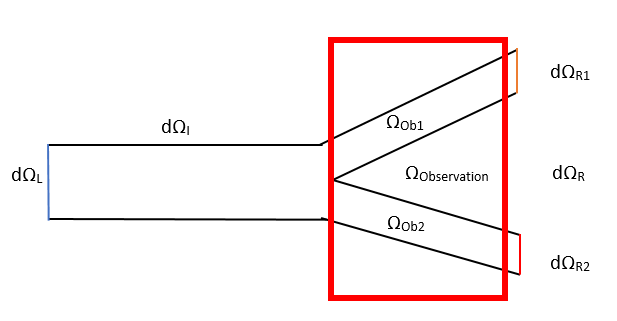
\includegraphics[scale=0.8]{observation.png}
	\caption{Domain of Interest}
	\label{Observation1}
\end{figure}
The first problem of interest is of the form:
\begin{align*}
&\min_{\Sta, w} \quad \frac{1}{2}|| \Sta -\widehat \Sta||^2_{L_2( \Sigma_{Ob})} + \frac{\beta}{2}||w||^2_{L_2(\Sigma)}\\
&\text{subject to:}\\
&\partial_t \rho = \nabla^2 \rho - \nabla \cdot (\rho \mathbf{w}) +\nabla \cdot (\rho \nabla V_{ext}) + \nabla \cdot \int_\Omega \rho(r) \rho(r') \nabla V_2(|r-r'|) dr' + w \quad  \text{in} \quad \Sigma\notag\\
& \rho = \rho_0 \quad \text{at} \quad t=0 \notag\\
& - \mathbf{j} \cdot \nor = \mathbbm{1}_{\partial \Omega_L}( C_{L1}  + C_{L2}\Sta) +\mathbbm{1}_{\partial \Omega_R} ( C_{R1}  + C_{R2}\Sta) +\mathbbm{1}_{\partial \Omega_I} 0 \ \quad \quad\qquad\qquad  \qquad \text{on} \quad \partial \Omega, 
\end{align*}
where $C_{L1}, C_{L2}, C_{R1}$, $C_{R2}$ are constants and $\mathbbm{1}$ is the indicator function of the set of interest. Considering Figure \ref{Observation1}, the stated non-constant flux boundary condition provides the option of describing a non-constant inflow on boundary $\partial \Omega_L$ and a non-constant outflow on $\partial \Omega_R$, while keeping a no flux condition on the rest of the boundary, denoted by $\partial \Omega_I$.
Furthermore, $\mathbf{j}$ satisfies:
\begin{align*}
\mathbf{j}=\nabla \rho - (\rho \mathbf{w}) +(\rho \nabla V_{ext}) +  \int_\Omega \rho(r) \rho(r') \nabla V_2(|r-r'|) dr'.
\end{align*}
Moreover, let $\widehat \Sta$ be defined such that:
\begin{align*}
\widehat \Sta = \mathbbm{1}_{ \Omega_{Ob1}} \tilde \Sta  +\mathbbm{1}_{ \Omega_{Ob2}} 0.
\end{align*}
This describes a desired state where the particle mass accumulates in the observation domain $\Omega_{Ob1}$ and no particles are found in $\Omega_{Ob1}$. Since observations are only taken on $\Omega_{Ob}$, there is no prescribed desired state on $\Omega / \Omega_{Ob}$.\\
The Lagrangian is of the form:
\begin{align*}
\mathcal{L}(\Sta,w,\Adjb,\Adjc ) &=\frac{1}{2} \int_0^T \int_{\Omega_{Ob}} (\Sta - \widehat \Sta)^2 dr dt + \frac{\beta}{2}\int_0^T \int_\Omega w^2 drdt \\
&+ \int_0^T \int_\Omega \bigg( \partial_t \rho - \nabla^2 \rho + \nabla \cdot (\rho \mathbf{w}) -\nabla \cdot (\rho \nabla V_{ext}) \\
&+ \nabla \cdot \int_\Omega \rho(r) \rho(r') \nabla V_2(|r-r'|) -w \bigg) \Adjb dr dt\\
&+ \int_0^T \int_{\partial \Omega} \bigg(  \bigg(-\nabla \rho+ (\rho \mathbf{w}) -(\rho \nabla V_{ext}) -  \int_\Omega \rho(r) \rho(r') \nabla V_2(|r-r'|) dr' \bigg)\cdot \nor\\
&  -\mathbbm{1}_{\partial \Omega_L}( C_{L1}  + C_{L2}\Sta) -\mathbbm{1}_{\partial \Omega_R} ( C_{R1}  + C_{R2}\Sta) -\mathbbm{1}_{\partial \Omega_I} 0 \bigg) \Adjc dr dt.
\end{align*}
The derivative of $\mathcal{L}$ with respect to $\rho$ is, as taken from the extended project, is:
\begin{align*}
&\mathcal{L}_\rho (\rho,{w},\Adjb,\Adjc)h=
\int_\Omega h(T) \Adjb(T) dr\\
&+ \int_0^T \int_\Omega \bigg( \mathbbm{1}_{ \Omega_{Ob}} (\rho- \widehat{\rho})  - \partial_t \Adjb  - \nabla \Adjb \cdot \mathbf{w}  - \nabla^2 \Adjb \notag 
+  \nabla \Adjb \cdot \nabla V_{ext}  \notag \\
&+ \int_\Omega (\nabla  \Adjb(r)+\nabla  \Adjb(r')) \rho(r') \nabla V_2(|r-r'|) dr'+ \int_{\partial \Omega} ( \Adjc(r') - \Adjb(r')) \rho(r')   \frac{\partial V_2(|r-r'|)}{\partial n} dr' \bigg) h dr dt \\
&+  \int_0^T\int_{\partial \Omega}  \bigg(
\bigg(\frac{\partial \Adjb }{\partial n} + \Adjb  \mathbf{w} \cdot \mathbf{n} - \Adjc \mathbf{w} \cdot \mathbf{n}  +  \Adjc \dfrac{\partial V_{ext}}{\partial n} - \Adjb \frac{\partial V_{ext}}{\partial n} + ( \Adjc - \Adjb)  \int_\Omega \rho(r') \frac{\partial V_2(|r-r'|)}{\partial n} dr'\\
& -\mathbbm{1}_{\partial \Omega_L} C_{L2} \Adjc   -\mathbbm{1}_{\partial \Omega_R} C_{R2} \Adjc \bigg)h + \bigg( \Adjc- \Adjb \bigg) \frac{\partial h}{\partial n} \bigg) dr dt =0.
\end{align*}
Then, from appropriate analysis we find that:
\begin{align*}
\Adjc = \Adjb,
\end{align*}
and therefore we get:
\begin{align*}
\mathbbm{1}_{\Omega_{Ob}}(\rho- \widehat{\rho})   - \partial_t  \Adjb  - \nabla \Adjb \cdot \mathbf{w}  - \nabla^2 \Adjb \notag 
+  \nabla \Adjb \cdot \nabla V_{ext}  \notag \\
+ \int_\Omega (\nabla  \Adjb(r)+\nabla  \Adjb(r')) \rho(r') \nabla V_2(|r-r'|) dr' &=0, \quad \text{in} \quad \Sigma, \\
\frac{\partial \Adjb }{\partial n}  -\mathbbm{1}_{\partial \Omega_L} C_{L2} \Adjb   -\mathbbm{1}_{\partial \Omega_R} C_{R2} \Adjb&=0, \quad \text{on} \quad \partial \Omega.
\end{align*}
In particular, this is:
\begin{align*}
\mathbbm{1}_{\Omega_{Ob1}}(\rho- \widehat{\rho}) +\mathbbm{1}_{\Omega_{Ob2}}\rho  - \partial_t  \Adjb  - \nabla \Adjb \cdot \mathbf{w}  - \nabla^2 \Adjb \notag 
+  \nabla \Adjb \cdot \nabla V_{ext}  \notag \\
+ \int_\Omega (\nabla  \Adjb(r)+\nabla  \Adjb(r')) \rho(r') \nabla V_2(|r-r'|) dr' &=0, \quad \text{in} \quad \Sigma, \\
\frac{\partial \Adjb }{\partial n}  -\mathbbm{1}_{\partial \Omega_L} C_{L2} \Adjb   -\mathbbm{1}_{\partial \Omega_R} C_{R2} \Adjb&=0, \quad \text{on} \quad \partial \Omega.
\end{align*}
The gradient equation is:
\begin{align*}
w = \frac{1}{\beta}\Adjb.
\end{align*}
Comparing this to the previous section, it can be observed that the gradient equations have opposite signs. This is due to a different construction of the Lagrangian.





The problem of interest is of the form:
\begin{align*}
&\min_{\Sta, \Con} \quad \frac{1}{2}|| \Sta -\hat \Sta||^2_{L_2(\partial Q_R)} + \frac{\beta}{2}|| \Con||^2_{L_2(Q)}\\
\text{subject to:}\\
&\partial_t \rho = \nabla^2 \rho - \nabla \cdot (\rho \mathbf{w}) +\nabla \cdot (\rho \nabla V_{ext}) + \nabla \cdot \int_\Omega \rho(r) \rho(r') \nabla V_2(|r-r'|) dr' + \Con \quad  \quad\text{in} \quad Q,\notag\\
& \rho = \rho_0 \quad \text{at} \quad t=0 \notag\\
& - \mathbf{j} \cdot \nor = \mathbbm{1}_{\partial \Omega_L}( C_{L1}  + C_{L2}\Sta) +\mathbbm{1}_{\partial \Omega_R} ( C_{R1}  + C_{R2}\Sta) +\mathbbm{1}_{\partial \Omega_I} 0, \quad  \quad\text{on} \quad \partial Q, 
\end{align*}
where $C_{L1}, C_{L2}, C_{R1}$, $C_{R2}$ are constants and $\mathbbm{1}$ is the indicator function of the set (the parts of the boundary) of interest.
Furthermore, $\mathbf{j}$ satisfies:
\begin{align*}
\mathbf{j}=\nabla \rho - (\rho \mathbf{w}) +(\rho \nabla V_{ext}) +  \int_\Omega \rho(r) \rho(r') \nabla V_2(|r-r'|) dr'.
\end{align*}
Moreover, let $\hat \Sta$ be defined such that:
\begin{align*}
\hat \Sta = \mathbbm{1}_{\partial \Omega_{R1}} \tilde \Sta  +\mathbbm{1}_{\partial \Omega_{R2}} 0.
\end{align*}

\subsection*{The Lagrangian}
The Lagrangian is of the form:
\begin{align*}
\mathcal{L}(\Sta,\Con,\Adja,\Adjc ) &= \int_0^T \int_{\partial \Omega_R} \frac{1}{2}(\Sta - \hat \Sta)^2 dr dt + \frac{\beta}{2}\int_0^T \int_\Omega \Con^2 drdt \\
&+ \int_0^T \int_\Omega \bigg( \partial_t \rho - \nabla^2 \rho + \nabla \cdot (\rho \mathbf{w}) -\nabla \cdot (\rho \nabla V_{ext}) + \nabla \cdot \int_\Omega \rho(r) \rho(r') \nabla V_2(|r-r'|) \bigg) \Adja dr dt\\
&+ \int_0^T \int_{\partial \Omega} \bigg(  \bigg(-\nabla \rho+ (\rho \mathbf{w}) -(\rho \nabla V_{ext}) -  \int_\Omega \rho(r) \rho(r') \nabla V_2(|r-r'|) dr' \bigg)\cdot \nor\\
&  -\mathbbm{1}_{\partial \Omega_L}( C_{L1}  + C_{L2}\Sta) -\mathbbm{1}_{\partial \Omega_R} ( C_{R1}  + C_{R2}\Sta) -\mathbbm{1}_{\partial \Omega_I} 0 \bigg) \Adjc dr dt.
\end{align*}

\subsection*{The Adjoint Equation}
The derivative of $\mathcal{L}$ with respect to $\rho$ is, as taken from the extended project:
\begin{align*}
&\mathcal{L}_\rho (\rho,\mathbf{w},p_\Omega,p_{\partial \Omega})h=
\int_\Omega h(T) \Adja(T) dr\\
&+ \int_0^T \int_\Omega \bigg(   - \partial_t \Adja  - \nabla \Adja \cdot \mathbf{w}  - \nabla^2 \Adja \notag 
+  \nabla \Adja \cdot \nabla V_{ext}  \notag \\
&+ \int_\Omega (\nabla  \Adja(r)+\nabla  \Adja(r')) \rho(r') \nabla V_2(|r-r'|) dr'+ \int_{\partial \Omega} ( \Adjc(r') - \Adja(r')) \rho(r')   \frac{\partial V_2(|r-r'|)}{\partial n} dr' \bigg) h dr dt \\
&+  \int_0^T\int_{\partial \Omega}  \bigg(
\bigg(\frac{\partial \Adja }{\partial n} + \Adja  \mathbf{w} \cdot \mathbf{n} - \Adjc \mathbf{w} \cdot \mathbf{n}  +  \Adjc \dfrac{\partial V_{ext}}{\partial n} - \Adja \frac{\partial V_{ext}}{\partial n} + ( \Adjc - \Adja)  \int_\Omega \rho(r') \frac{\partial V_2(|r-r'|)}{\partial n} dr'\\
&\mathbbm{1}_{\partial \Omega_R} (\rho- \hat{\rho}) -\mathbbm{1}_{\partial \Omega_L} C_{L2} \Adjc   -\mathbbm{1}_{\partial \Omega_R} C_{R2} \Adjc \bigg)h + \bigg( \Adjc- \Adja \bigg) \frac{\partial h}{\partial n} \bigg) dr dt =0.
\end{align*}
Then, from appropriate analysis we find that:
\begin{align*}
\Adjc = \Adja,
\end{align*}
and therefore we get:
\begin{align*}
- \partial_t  \Adja  - \nabla \Adja \cdot \mathbf{w}  - \nabla^2 \Adja \notag 
+  \nabla \Adja \cdot \nabla V_{ext}  \notag \\
+ \int_\Omega (\nabla  \Adja(r)+\nabla  \Adja(r')) \rho(r') \nabla V_2(|r-r'|) dr' &=0, \quad \text{in} \quad Q, \\
\frac{\partial \Adja }{\partial n}+ \mathbbm{1}_{\partial \Omega_R} (\rho- \hat{\rho}) -\mathbbm{1}_{\partial \Omega_L} C_{L2} \Adja   -\mathbbm{1}_{\partial \Omega_R} C_{R2} \Adja&=0, \quad \text{on} \quad \partial Q.
\end{align*}
Again, in particular the boundary condition is:
\begin{align*}
\frac{\partial \Adja }{\partial n}+ \mathbbm{1}_{\partial \Omega_{R1}}(\rho- \tilde{\rho} -C_{R2} \Adja) + \mathbbm{1}_{\partial \Omega_{R2}} (\Sta-C_{R2} \Adja) - \mathbbm{1}_{\partial \Omega_L} C_{L2} \Adja   &=0, \quad \text{on} \quad \partial Q.
\end{align*}

	

\section{Numerical Methods}	

In order to solve the PDE-constrained optimization problem (\ref{sysPDEconstroptiAndNonlocal1}), it is necessary to solve the first-order optimality conditions (\ref{sysFirstOderOptimalityNonLocal1}). Therefore, methods of time and space discretization, as well as a method for solving the system of PDEs are needed. One challenge specific to this problem is the final time condition in the adjoint equation, which means that it is a boundary value problem in time as well as in space. 	
The numerical methods that are needed to solve (\ref{sysFirstOderOptimalityNonLocal1}) are introduced in this section.
A lot of research has been done on numerical methods for solving linear PDE-constrained optimization problems, as demonstrated in \cite{DeLosReyesOptimization}, \cite{CarraroDirectIndirectMultipleShooting} and \cite{TroeltzschFredi2010OCoP}.
New approaches to solving the optimality system (\ref{sysPDEconstroptiAndNonlocal1}) are needed because of the non-linear, non-local nature of the particle interaction term in the PDE-constraint. Standard methods are no longer sufficient to solve this type of problem, as discussed in this section.

\subsection{Pseudospectral Methods} \label{secPSMTheory1}

Pseudospectral methods on non-periodic domains are based on polynomial interpolation on non-equispaced points.  
Typically, Chebyshev points $\{x_j\}$ are chosen as collocation points on $[-1,1]$, which are defined as:
\begin{align}\label{defChebyshevPoints}
x_j= \cos\bigg(\frac{j \pi}{N}\bigg), \quad j=0,1,...,N,
\end{align}	
see \cite{bibTrefethen}.
These points are clustered at the endpoints of the interval, and sparse around $0$. Using this approach, the points are distributed from $1$ to $-1$, which is counter-intuitive. Therefore, in the code library \cite{GoddardPseudospectralCode1}, which is used in producing the results of this report, the Chebyshev points are automatically flipped back to run from $-1$ to $1$. Moreover, a linear map takes the points from the computational domain $[-1,1]$ to any domain $[a,b]$ of interest.
Interpolation on the Chebyshev grid is done using barycentric Lagrange interpolation, derived in \cite{bibTrefethenBerrut1}. The barycentric formula is:
\begin{align*}
p_N(x)= \frac{\displaystyle \sum_{k=0}^N \frac{\tilde w_k}{x-x_k}f(x_k)}{\displaystyle \sum_{k=0}^N \frac{\tilde w_k}{x-x_k}},
\end{align*}
where the weights are defined as:
\begin{align*}
\tilde w_j = (-1)^j d_j, \quad d_j = 
\left \{
\begin{tabular}{c}
$\frac{1}{2}$ \text{for} $j=0$, $j=N$, \\
$1$ \text{otherwise}, \phantom{abksla} 
\end{tabular}
\right .
\end{align*}
see \cite{bibTrefethenBerrut1} and \cite{GoddardPseudospectralCode1}.

The derivation of the Chebyshev differentiation matrices is described below, following the presentation in \cite{bibTrefethen}.
The function of interest, $f$, is evaluated at the Chebyshev points $\{x_j\}$ and a grid function, $f_j := f(x_j)$, is defined.
There exists a unique polynomial of degree $\leq N$ that can be used to interpolate $f$ on the grid points $x_j$. The polynomial $p$ satisfies, by definition, the following relationship:
\begin{align}\label{eqnptov1}
p(x_j)=f_j,
\end{align}
so that the residual $p(x_j) -f_j$ is zero at these points. Therefore, this method is called a collocation method, see \cite{Boyd1}. 
Once such a polynomial $p$ is found, it can be differentiated and the following relationship is defined:
\begin{align*}
w_j = p'(x_j).
\end{align*} 	
This relationship can be rewritten as a multiplication of $f_j$ by a $(N+1) \times (N+1)$ matrix, denoted by $D$, as follows:
\begin{align*}
w_j= D f_j,
\end{align*}
using (\ref{eqnptov1}).
A $(N+1) \times (N+1)$ differentiation matrix $D$ has the following entries, compare with \cite{bibTrefethen}:
\begin{align*}
(D)_{00}&= \frac{2N^2 +1}{6},\\
(D)_{NN}&= -\frac{2N^2 +1}{6},\\
(D)_{jj}&= -\frac{x_j}{2(1-x_j^2)}, \quad j=1,...,N-1,\\
(D)_{ij}&= \frac{c_i}{c_j} \frac{(-1)^{i+j}}{(x_i-x_j)}, \quad i \neq j, \quad i,j=0,...,N,
\end{align*} 	
where 
\begin{align*}
c_i =\left\{\begin{array}{l} 2, \quad i=0 \text{   or   }N, \\1, \quad \text{otherwise.}\end{array}\right.
\end{align*}	
The second derivative is represented by the second differentiation matrix $D_2$, which can be found by squaring the first differentiation matrix; $D_2=D^2$, and more generally the $j^{th}$ differentiation matrix is found as follows:
\begin{align*}
D_j=D^j.
\end{align*}
However, in \cite{GoddardPseudospectralCode1}, the exact coefficients, derived in a similar way as above for $D$, are used to compute $D_2$, since it is more accurate than squaring $D$.
\\
In order to extend the definition of the differentiation matrices to two-dimensional grids, a so-called tensor product grid has to be defined. First, Chebyshev points $x_j$, for $j=1,...,n$, on the $x$-axis and another set of Chebyshev points $y_i$, for $i=1,...,m$ on the $y$-axis are taken, both between $[-1,1]$. Then the following two vectors are defined:
\begin{align*}
\mathbf{x}_{K}=(x_1,x_1,...,x_1,x_2,x_2,...,x_2,...,x_n,x_n,...,x_n)^T,\\
\mathbf{y}_{K}=(y_1,y_2,...,y_m,y_1,y_2...,y_m,.....,y_1,y_2,...,y_m)^T.
\end{align*} 
In $\mathbf{x}_K$, each $x_j$ is repeated $m$ times, while $\mathbf{y}_K$, each sequence $y_1,y_2,...,y_m$ is repeated $n$ times. The total length of each vector is $n \times m$. 
These vectors are defined, so that the set $(\mathbf{x}_K,\mathbf{y}_K)$ is a full set of all Chebyshev points on the two-dimensional tensor grid.
Note that the points are clustered around the boundary of the two-dimensional grid and sparse in the middle of the grid.
These Kronecker vectors can be used to find the Chebyshev differentiation matrices for two-dimensional problems as follows, compare to \cite{bibTrefethen}. For a first derivative $D$ in the $x$ direction, a Kronecker product is taken of the one-dimensional Chebyshev differentiation matrix with the identity, as demonstrated here with three points:
\begin{align*}
D_x&=I \otimes D = 
\begin{pmatrix}
1 & 0 & 0\\
0 & 1 & 0 \\
0 & 0 & 1
\end{pmatrix}
\otimes
\begin{pmatrix}
d_{11} & d_{12} & d_{13}\\
d_{21} & d_{22} & d_{23} \\
d_{31} & d_{32} & d_{33}
\end{pmatrix}
\\&=
\begin{pmatrix}
d_{11} & d_{12} & d_{13} & & &  & & &\\
d_{21} & d_{22} & d_{23} & & & & & & \\
d_{31} & d_{32} & d_{33} & & & & & & \\
& & &d_{11} & d_{12} & d_{13} & & &\\
& & &d_{21} & d_{22} & d_{23}  & & &\\
& & &d_{31} & d_{32} & d_{33} & & &\\
 & & & & & &d_{11} & d_{12} & d_{13}\\
& & & & & &d_{21} & d_{22} & d_{23}  \\
& & & & & &d_{31} & d_{32} & d_{33} 
\end{pmatrix},
\end{align*}
where the block structure matches the repetition of each $x_j$ in $\mathbf{x}_K$.
The second derivative with respect to $x$, $D_{xx}$ can be found by using $D_2$ instead of $D$ in this calculation. 
The derivative with respect to $y$ is found by taking the Kronecker product the other way around:
\begin{align*}
D_y&=D \otimes I = 
\begin{pmatrix}
d_{11} & d_{12} & d_{13}\\
d_{21} & d_{22} & d_{23} \\
d_{31} & d_{32} & d_{33}
\end{pmatrix}
\otimes
\begin{pmatrix}
1 & 0 & 0\\
0 & 1 & 0 \\
0 & 0 & 1
\end{pmatrix}
\\&=
\begin{pmatrix}
d_{11} & & & d_{12} & & & d_{13} & & \\
& d_{11} & & & d_{12} & & &  d_{13} & \\
& & d_{11} & & &  d_{12} &  & & d_{13}\\
d_{21} & & & d_{22} & & & d_{23} & & \\
& d_{21} & & & d_{22} & & &  d_{23} & \\
& & d_{21} & & &  d_{22} &  & & d_{23}\\
d_{31} & & & d_{32} & & & d_{33} & & \\
& d_{31} & & & d_{32} & & &  d_{33} & \\
& & d_{31} & & &  d_{32} &  & & d_{33}\\
\end{pmatrix},
\end{align*}
which now matches the repetition of each $y_1,...y_m$ in $\mathbf{y}_K$.
The Chebyshev differentiation of the Laplacian is given by: $L=I  \otimes D_2 + D_2 \otimes I$.
\\
\\
In order to evaluate integrals in a similar way, the so-called Clenshaw--Curtis quadrature is used, which is derived in \cite{ClenCurt1}.
This is, for the integral over a smooth function $f$:
\begin{align}\label{eqnClenCurtQuad}
\int_{-1}^1 f(x)dx = \sum_{k=0}^N w_kf(x_k),
\end{align}
where the weights are defined as:
\begin{align*}
w_j = \frac{2d_j}{N}
\left \{
\begin{tabular}{c}
$1- \displaystyle \sum_{k=1}^{(N-2)/2} \frac{2 \cos(2kt_j)}{4k^2-1} - \frac{\cos(\pi j)}{N^2 -1} \quad \quad\text{for $N$ even}$,\\
$1- \displaystyle \sum_{k=1}^{(N-2)/2} \frac{2 \cos(2kt_j)}{4k^2-1} \quad \quad \quad \quad \quad \quad \ \ \ \text{for $N$ odd}$,
\end{tabular}
\right .
\end{align*}
see \cite{GoddardPseudospectralCode1}.

The advantage of Spectral Methods is that, for smooth functions, the convergence is exponential, see \cite{Boyd1}:
\begin{align*}
\text{Pseudospectral Error} \approxeq O \bigg[ \bigg( \frac{1}{N} \bigg)^N \bigg].
\end{align*}


A good overview on spectral methods is given in \cite{bibTrefethen} and a more in depth discussion can be found in \cite{Boyd1}.


\subsection{Comparison with FEM and FDM} \label{secCompareFEMFDMPDM}

In this section the advantages and disadvantages of pseudospectral methods over finite element methods (FEM) and finite difference methods (FDM) are discussed, compare to \cite{Boyd1}.
The main difference between pseudospectral methods (PSM) and the other two methods is that PSM uses global basis functions on all Chebyshev points, while FEM uses local basis functions and FDM uses local, low order polynomials.
\\
Finite difference methods use overlapping sequences of polynomials to approximate the solution of the problem. They are easy to implement and less costly per degree of freedom. However, they are also less accurate than PSM.
\\
The basis functions used in FEM methods are generally of fixed, low degree and more accuracy is achieved through refinement of the elements; either in the whole domain or in regions where the problem is more difficult to solve.
In comparison, the global basis function used in PSM are generally of higher degree than the ones in FEM. Furthermore, in order to refine the method, the degree of the polynomial can be increased.
\\
In general, FEM results in large sparse matrix systems, which in many cases can be solved by exploiting their structure. It is also easily applied to complex domains, due to the shape of the elements.
However, the disadvantage of FEM is low accuracy of solutions, due to the low degree of the polynomial basis functions. Furthermore, the sparsity property of the matrix systems is compromised when the PDEs involve nonlocal terms. Therefore, PSM are advantageous in this type of problems, since small dense matrices are utilized. 
 As discussed in \cite{FEMIntegroPaper}, an adaptive FEM method can be used to solve an integro-differential PDE-constrained optimal control problem. However, the accuracy achieved is mainly of order $O(10^{-2})$ and maximal $O(10^{-4})$, for a two dimensional problem with $N$ nodes, where $N$ is between $N=3549$ and $50421$. The time step is $dt=0.05$. Furthermore, Dirichlet boundary conditions are used, which avoids applying more realistic no-flux boundary conditions. These no-flux boundary conditions are difficult to apply in the FEM context, because they are nonlocal as well. Within the existing code framework \cite{GoddardPseudospectralCode1}, these boundary conditions are straightforward to apply.
The disadvantages of PSM are that they are more computationally expensive and the domain is required to be smooth.
However, as discussed in \cite{Boyd1}, if the accuracy of PSM with $N=10$ is to be achieved by FEM or FDM, a 10th order method has to be chosen with an error of $O(h^{10})$.
All in all, PSM is the best method for solving PDE-contrained optimization problems involving integro-PDEs.

\subsection{Exact Solutions} \label{secExactSolsDiffusion1}

For some relatively simple PDE-constrained optimization problems it is possible to construct exact solutions to the first-order optimality system. This is an important aspect in the development of new numerical methods, since these problems can be used as test problems for the numerical method and the exact error can be measured. The considered test problem is a simplified version of (\ref{sysPDEconOpti1}), and therefore testing the numerical method on this problem is a step towards solving (\ref{sysPDEconOpti1}). In this section, the construction of an exact solution for the following problem is derived, where the PDE constraint is the forced heat equation on $\Omega =[-1,1]$:
\begin{align}\label{sysOptimalHeating1}
&\min_{\rho,u} \quad \frac{1}{2}\norm{\rho- \hat{\rho}}_{L_2}^2 + \frac{\beta}{2} \norm{u}_{L_2}^2,\\
&\text{subject to:}\notag 
\notag \\
&\partial_t \rho - \Delta \rho - u=0,  \quad \text{in} \quad \Omega,\notag 
\notag \\
&\rho(r,0)=\rho_0(r),\notag 
\notag \\
& \rho(r,t)=0, \quad  \quad \quad \quad \ \text{on} \quad \partial \Omega. \notag 
\end{align}
Note that $u$ is now the control variable, comparable to $\mathbf{w}$ in (\ref{sysPDEconOpti1}).
The first-order optimality system for this PDE-constrained optimization problem is:
\begin{align} \label{sysPotimaltiyheatequn1}
\textbf{Adjoint Equation} \notag \\
\partial_t p + \Delta p -\rho +\hat{\rho} &=0 \ \ \ \quad \quad \quad \text{in} \quad \Omega,  \\
p(r,T) &= 0 \notag\\
p(r,t) &=0 \quad \quad\quad\quad \text{on} \quad \partial\Omega, \notag\\
\textbf{Gradient Equation} \notag \\
\beta u  - p  &=0 \quad \quad\quad\quad \ \text{in} \quad \Omega, \notag \\
\textbf{Forward Problem} \notag \\
\partial_t \rho - \Delta \rho - u &=0 \ \quad \quad\quad\quad \text{in} \quad \Omega, \notag \\ 
\rho(r,0)&=\rho_0(r) \notag \\
\rho(r,t) &=0 \quad \quad\quad\quad \ \text{on} \quad \partial \Omega \notag. 
\end{align}
This follows almost directly from taking the relevant terms from the optimality system (\ref{sysFirstOderOptimality1}).
The solution to this system is derived in one and two dimensions, as well as for Dirichlet and Neumann boundary conditions.
\newline
\newline
In order to construct a full solution to the optimality system, the following steps have to be taken. At first, an expression for $p$ has to be chosen, such that the boundary conditions for the adjoint equation, as well as the final-time condition, are satisfied.
In a second step, this is substituted into the gradient equation to find $u$. The resulting expression can be used in the state equation to solve for $\rho$. Finally, once all three variables are defined, the adjoint equation can be used to solve for $\hat \rho$.
A functional form for $p$, satisfying Dirichlet boundary conditions and the final time condition is:
\begin{align*}
p(r,t) = \bigg( e^T -e^t \bigg) \cos(\pi r /2).
\end{align*}
Substituting this into the gradient equation gives:
\begin{align*}
u(r,t) = \frac{1}{\beta}\bigg( e^T -e^t \bigg) \cos(\pi r /2).
\end{align*}
Substituting $u$ into the state equation results in a decoupled PDE for $\rho$ that can be solved:
\begin{align}\label{eqnStateEqnDiff1DExact1}
\partial_t \rho - \partial_{r} \rho=\frac{1}{\beta}\bigg( e^T -e^t \bigg) \cos(\pi r /2).
\end{align}
Assuming a solution of the form: 
\begin{align*}
\rho(r,t)= \bigg(a +be^t\bigg)\cos(\pi r /2),
\end{align*}
and substituting it into (\ref{eqnStateEqnDiff1DExact1}) gives:
\begin{align*}
be^t\cos(\pi r /2) + \frac{\pi^2}{4}\bigg(a +be^t\bigg)\cos(\pi r /2)=\frac{1}{\beta}\bigg( e^T -e^t \bigg) \cos(\pi r /2),
\end{align*}
which results in:
\begin{align*}
\bigg(b+\frac{\pi^2}{4}b + \frac{1}{\beta} \bigg)e^t + \frac{\pi^2}{4}a-\frac{1}{\beta} e^T  =0.
\end{align*}
Therefore, $\displaystyle b=-\frac{1}{(1+\frac{\pi^2}{4}) \beta}$ and $ \displaystyle a=\frac{4}{\beta \pi^2}e^T$, and so $\rho$ becomes:
\begin{align*}
\rho(r,t)= \bigg(\frac{4}{\beta \pi^2}e^T -\frac{1}{(1+\frac{\pi^2}{4}) \beta}e^t\bigg)\cos(\pi r /2).
\end{align*}
The expressions for $\rho$ and $p$ can be substituted into the adjoint equation, to solve for $\hat \rho$:
\begin{align*}
e^t \cos(\pi r/2) + \frac{\pi^2}{4}\bigg( e^T -e^t \bigg) \cos(\pi r /2) = \hat \rho - \bigg(\bigg(\frac{4}{\beta \pi^2}e^T -\frac{1}{(1+\frac{\pi^2}{4}) \beta}\bigg)\cos(\pi r /2) \bigg).
\end{align*}
This gives:
\begin{align*}
\hat \rho(r,t)=\bigg( \bigg( \frac{4}{\beta \pi^2}+ \frac{\pi^2}{4} \bigg) e^T + \bigg(1- \frac{\pi^2}{4}  -\frac{1}{(1+\frac{\pi^2}{4}) \beta} \bigg) e^t\bigg)  \cos(\pi r /2) .
\end{align*}
This solution can be used for Neumann boundary conditions as well, when considered on an interval $[-2,2]$. This is due to the fact that $\cos(\pi r/2)$ evaluated at $-2,2$ is equal to $-1$ and $1$ respectively, which is exactly at its stationary points. Therefore, the Neumann boundary conditions are satisfied at these points.
Instead, the approach used in the numerical experiments below is to slightly change the calculations above to derive the following exact solutions for $\rho$, $p$ and $\hat \rho$ for solving (\ref{sysOptimalHeating1}) with Neumann boundary conditions:
\begin{align*}
p(r,t) &=\bigg( e^T -e^t \bigg) \cos(\pi r),\\
\rho(r,t) &= \bigg( \frac{1}{\pi^2 \beta}e^T - \frac{1}{(1+\pi^2)\beta}e^t\bigg)\cos(\pi r),\\
\hat \rho(r,t) &= \bigg( \bigg(\pi^2 + \frac{1}{\pi^2 \beta}\bigg)e^T + \bigg( 1- \pi^2 - \frac{1}{(1+\pi^2)\beta}\bigg)e^t \bigg) \cos(\pi r).
\end{align*}
Furthermore, these calculations can be done equivalently for two or more dimensional problems. 
The exact solution to the two-dimensional problem (\ref{sysOptimalHeating1}) with Dirichlet boundary conditions is:
\begin{align*}
p(r,t) &= \bigg( e^T -e^t \bigg) \cos(\pi x /2)\cos(\pi y /2),\\
\rho(r,t) &= \bigg(\frac{2}{\beta \pi^2}e^T -\frac{4}{(4+2\pi^2) \beta}e^t\bigg)\cos(\pi x /2)\cos(\pi y /2),\\
\hat \rho (r,t) &=\bigg( \bigg( \frac{2}{\beta \pi^2}+ \frac{\pi^2}{2} \bigg) e^T + \bigg(1- \frac{\pi^2}{2}  -\frac{4}{(4+2\pi^2) \beta} \bigg) e^t\bigg)  \cos(\pi x /2)\cos(\pi y /2),
\end{align*}
where $r=(x,y)$.
Finally, the exact solution to the two-dimensional problem (\ref{sysOptimalHeating1}) with Neumann boundary conditions is:
\begin{align*}
p(r,t)&= \bigg( e^T -e^t \bigg) \cos(\pi x )\cos(\pi y),\\
\rho(r,t) &= \bigg(\frac{1}{2\beta \pi^2}e^T -\frac{1}{(1+2\pi^2) \beta}e^t\bigg)\cos(\pi x )\cos(\pi y ),\\
\hat \rho (r,t) &=\bigg( \bigg( \frac{1}{\beta \pi^2}+ 2\pi^2 \bigg) e^T + \bigg(1- 2\pi^2  -\frac{1}{(1+2\pi^2) \beta} \bigg) e^t\bigg)  \cos(\pi x)\cos(\pi y).
\end{align*}
The exact solutions presented here for Dirichlet boundary conditions, for $d$ dimensions, can be found in \cite{GuettelPearson1}.


\subsection{Multiple Shooting Method}	

Boundary value problem (BVP) solvers, such as \texttt{bvp4c}, are designed to treat BVPs in time, see \cite{bvp4cPaper1}. Therefore, they are not equipped to deal with BVPs in both space and time. A method has to be developed that circumvents using BVP solvers and uses initial value problem (IVP) solvers instead. This strategy is called multiple shooting and the theoretical derivation of a multiple shooting approach for PDE-constrained optimization problems can be found in \cite{CarraroIndMultipleShooting} and \cite{CarraroDirectIndirectMultipleShooting}.
\\
In this section, the numerical method is described at the different stages of its development. 
The PDE constraint considered has either Dirichlet or Neumann boundary conditions in space. The problem is treated in one and two dimensions. In order to initiate the development of the method, a simpler PDE constrained optimization problem is considered at first. Once the method is established for the simpler problem, the non-local term is added. After that, two dimensional problems are considered.

\subsubsection*{One-Dimensional Diffusion} \label{secNumericsOneDDiffusion1}
One of the simplest cases of a PDE-constrained optimization problem is heat control in one dimension. The PDE constraint involved is the forced heat equation, and the PDE-constrained optimisation problem (\ref{sysOptimalHeating1}), derived in Section \ref{secExactSolsDiffusion1}, is used, and the derived optimality system is treated below. 

The first step in solving this optimality system is to substitute the gradient equation into the heat equation for $u$ and rearranging the equations to only have the time derivative on the left-hand side.
This results in a coupled system of PDEs: 
\begin{align}\label{sysOneDimHeatEqunOptisys1}
\partial_t \rho(r,t) &= \partial_{rr}\rho(r,t) + \frac{1}{\beta}p(r,t),\\
\partial_t p(r,t) &= - \partial_{rr} p(r,t) + \rho(r,t) -\hat{\rho}(r,t), \notag \\
\text{Initial } & \text{and  Final-Time Conditions:}\notag\\
\rho(r,0)&=\rho_0(r),\notag\\
p(r,T) &=0,\notag\\
\text{Dirich} &\text{let  Boundary Conditions:}\notag\\
\rho(r,t) &=0,\quad \text{on} \quad \partial \Omega,\notag\\
p(r,t) &=0,\quad \text{on} \quad \partial \Omega,\notag
\end{align}
where $r \in [a,b]$ and $t \in [0,T]$.
This system is considered as a test problem, since exact solutions for $\rho$ and $p$ are known. Therefore, the exact error of the numerical method can be determined at all points in space and time. The derivation of the exact solutions are discussed in Section \ref{secExactSolsDiffusion1}.

The method that is used to solve this system of PDEs is called the shooting method.
The procedure is to first discretize the problem in space, that is to replace the space derivatives with the appropriate Chebyshev differentiation matrices, as defined above. Then the problem reduces to a coupled system of ODEs, which can be solved using an ODE solver, such as the Matlab solver \texttt{ode15s}. The challenge is that the optimality system is a boundary value problem in time, since the adjoint equation has a final time condition in $p$. 
Therefore, the first idea is to create a guess for the initial condition $p_0(r)$, solve the coupled ODE system using this guess, extracting the computed $p$ value at the final time, $p_{co}(T)$ and measuring the error between the computed $p_{co}$ and the exact $p_{ex}$:
\begin{align*}
e= \norm{p_{co}(T) - p_{ex}(T)}.
\end{align*}
The final step in this procedure is to minimize this error by varying $p_0(r)$, using an in-built Matlab optimization routine, such as \texttt{fsolve}.
This is easily implemented in Matlab, see Appendix \ref{ShootingTest1DiffusionLineBlowsUp}.
However, the problem with this approach is that the adjoint equation, written in this form, is not well posed. The solution to this system blows up in finite time, which is caused by the negative diffusion term in the PDE for $p$.\\

Therefore, the adjoint equation has to be rewritten. This is done by rescaling time as
\begin{align*}
\tau=T+t_0-t,
\end{align*}
which causes the adjoint equation to run backwards in time from $T$ to $t_0=0$. This changes the final time condition for $p$ at time $t=T$, $p(T)=0$, into an initial condition at time $\tau =0$, ${p}(0)=0$.
The optimality system is then:
\begin{align} \label{sysOptimDiffAdjBW1}
\partial_t \rho(r,t) &= \partial_{rr} \rho(r,t) + \frac{1}{\beta}{p}(r,t), \\
\partial_t {p}(r,\tau) &=\partial_{rr} {p}(r,\tau) - \rho(r,\tau) +\hat{\rho}(r,\tau), \notag \\
\text{Initial   } & \text{ Conditions:} \notag  \\
 \rho(r,0)&=\rho_0(r),  \quad \text{for} \quad t=0,\notag \\
{p}(r,0) &=0, \quad \text{for} \quad \tau=0,\notag \\
\text{Dirich} &\text{let Boundary Conditions:} \notag \\
\rho(a,t) &=\rho(b,t)=0, \notag \\
{p}(a,\tau) &={p}(b,\tau)=0, \notag 
\end{align} 
where $t \in [t_0,T]$ and $\tau \in [T,t_0]$.
This is now well posed. However, the issue with this rewritten system is that information about $\rho$ at later times is needed to solve the adjoint equation and ${p}$ values for earlier times are needed to solve the state equation, while neither of these information is available. Figure \ref{ShootingMethod1} visualises this problem. The initial conditions for $\rho$ and $p$ are represented as a green and blue dot respectively. Time $t$ is represented by the green arrow, while time $\tau$, the backwards time, is represented by a blue arrow. In order to test whether this approach works, the exact solution for $\rho$ and $q$ can be used, where information is missing. Then the problem is a decoupled system of PDEs, which is straightforward to solve.  


%\begin{figure}[h] 
%		\vspace{-20pt}
%	\centering
%	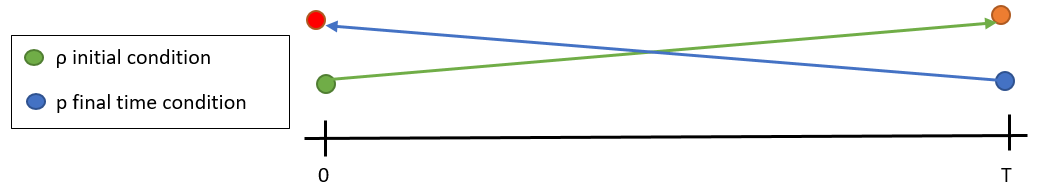
\includegraphics[scale=0.85]{FullSol.png}
%		\vspace{-10pt}
%    \caption{Solving a coupled system of PDEs on $[0,T]$.} 
%    \label{ShootingMethod1}
%    	\vspace{-10pt}
%\end{figure}


In order to replace the missing information, as illustrated above, interpolation is used. Since interpolation using only the endpoints of the interval $[t_0,T]$ would be highly inaccurate, a strategy, called multiple shooting, is exploited in this section. 
The time interval is divided into a number of $n$ subintervals, such that $t_0 < t_1<t_2<...<t_n=T$. The subintervals are denoted by $I_i$, where $i=0,1,...,n-1$. The values for $\rho$ and ${p}$ at these times constitute the initial guess. The discretization of the time interval and initial guesses for $\rho$ and $p$ are illustrated in Figure \ref{ShootingMethod2}. The initial guess can be obtained by different methods, which will be discussed in a later section.

%\begin{figure}[h] 
%	\centering
%	\vspace{-10pt}
%	\includegraphics[scale=0.9]{FullDiscr.png}
%		\vspace{-10pt}
%	\caption{Discretizing the time interval and obtain initial guesses for $\rho$ and $q$.} 
%	\label{ShootingMethod2}
%	\vspace{-10pt}
%\end{figure}

In a first step, these initial guesses are chosen to be the known exact solutions to $\rho$ and ${p}$ at the specified times $t_i$. 
The optimality system (\ref{sysOptimDiffAdjBW1}) is solved on each of the $I_i$, by considering the upper and lower bound of the subinterval, $t_i$ and $t_{i+1}$ instead of the global bounds $t_0$ and $T$. The new backward running time is defined, equivalently to above, as $\tilde\tau =t_{i+1}+t_i-t$, and the system becomes:
\begin{align} \label{sysOptimDiffAdjBW2}
\partial_t \rho(r,t) &= \partial_{rr}\rho(r,t) + \frac{1}{\beta}{p}(r,t), \\
\partial_t {p}(r,\tilde\tau) &= \partial_{rr}{p}(r,\tilde\tau) - \rho(r,\tilde\tau) +\hat{\rho}(r,\tilde\tau), \notag \\
\text{Initial   } & \text{ Conditions:} \notag  \\
\rho(r,t_i)&=\rho_{t_i}, \quad \ \ \text{for} \ \quad t=t_i, \notag \\
{p}(r,t_{i+1}) &=p_{t_{i+1}}, \quad \text{for} \quad \tilde t=t_{i+1}, \notag \\
\text{Dirich} &\text{let  Boundary Conditions:} \notag \\
\rho(a,t) &=\rho(b,t)=0, \notag \\
{p}(a,\tilde\tau) &={p}(b,\tilde\tau)=0, \notag 
\end{align} 
where $t \in I_{i}=[t_i,t_{i+1}]$.
On each subinterval, both $\rho$ and ${p}$ are interpolated between their known values at $t_i$ and $t_{i+1}$, and the result is used to provide $\rho$ at a later time step, to solve the adjoint equation, as well as ${p}$ at an earlier time step, to solve the state equation. 
\newline
\newline
In order to implement the strategy, (\ref{sysOptimDiffAdjBW2}) is evaluated on each time interval $I_i=[t_i,t_{i+1}]$, using interpolation for $\rho$ in the adjoint equation and for $ {p}$ in the state equation to provide the missing information.

%\begin{figure}[h] 
%	\centering
%	\vspace{-10pt}
%	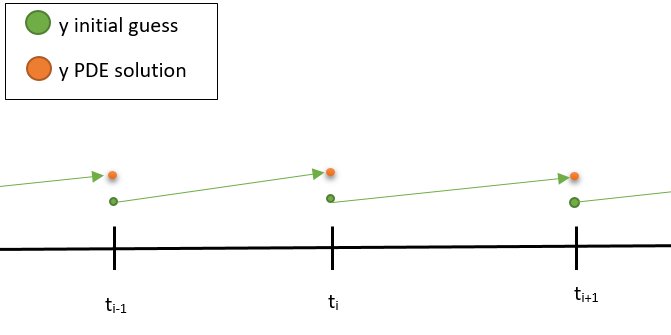
\includegraphics[scale=0.9]{rhoSol.png}
%	\caption{Solution strategy for $\rho$.} 
%	\label{ShootingMethod3}
%\end{figure}
%
%\begin{figure}[h] 
%	\centering
%	\vspace{-20pt}
%	\includegraphics[scale=0.9]{pSol.png}
%	\caption{Solution strategy for $p$.} 
%	\label{ShootingMethod4}
%	\vspace{-10pt}
%\end{figure}

As can be observed in Figure \ref{ShootingMethod3}, the value of $\rho$, taken from the ODE solver, at $t_{i+1}$ is compared to $\rho$ at $t_{i+1}$, which is the initial guess for solving (\ref{sysOptimDiffAdjBW2}) on the next interval $I_{i+1}=[t_{i+1},t_{i+2}]$:
\begin{align}\label{eqnErrorINitoptiguess}
e= \norm{g_{init}-g_{sol}},
\end{align} 
where $g_{init}=(g_1,g_2,...g_n)$ is a vector of initial guesses for $\rho$ on all $n$ time points and $g_{sol}$ is the vector of PDE solutions associated with the initial guesses on all time points.
This provides an error measure of the quality of the set of initial guesses $g_{init}$ for $\rho$. This error calculation is repeated for ${p}$, as illustrated in Figure \ref{ShootingMethod4}. However, since ${p}$ is running backwards in time, the solution to the ODE solver provides the value for ${p}$ at $t_i$, the lower bound on the considered interval $I_i$, which is then compared with the initial guess for ${p}$ for the previous interval $I_{i-1}=[t_{i-1},t_i]$.
Note that for this solution strategy any ODE solver can be used to solve the discretized PDE on each subinterval. Furthermore, while pseudospectral methods are the best method for PDE-constrained optimization problems involving integro-PDE constraints, as discussed in Section \ref{secCompareFEMFDMPDM}, it is in principle possible to use other time or space discretization methods.
\subsubsection*{One-Dimensional Diffusion with a Non-Local Term}\label{secOneDDiffusionNonlocalOptim1}
The problem (\ref{sysOptimalHeating1}) is extended by adding a non-local term to the forced heat equation. This non-local term is the two body interaction term that is introduced in Section \ref{secOptimalitySysNonLocal1}.
The one dimensional PDE-constrained optimization problem is:
\begin{align}
&\min_{\rho,u} \quad \frac{1}{2}\norm{\rho- \hat{\rho}}_{L_2}^2 + \frac{\beta}{2} \norm{u}_{L_2}^2,\\
&\text{subject to:}\notag 
\notag \\
&\partial_t \rho - \Delta \rho - u - \nabla \cdot \rho(r) \int_\Omega \nabla V_2(|r-r'|) \rho(r')dr'=0,  \quad \text{in} \quad \Omega,\notag 
\notag \\
&\rho(r,0)=\rho_0(r),\notag 
\notag \\
& \rho(r,t)=0, \quad \text{on} \quad \partial \Omega. \notag 
\end{align}
The first-order optimality system, including the non-local term, is:
\begin{align}\label{sysoptinonlocandheat1D}
\textbf{Adjoint Equation}  \\
\partial_t  p  + \partial_{rr} p + \int_\Omega \bigg(\partial_r  p(r)+\partial_{r'}  p(r')\bigg) \rho(r') \partial_r V_2(|r-r'|) dr' &=(\rho- \hat{\rho})  \quad \text{in} \quad \Omega, \notag \\
p(T) &= 0 \notag\\
p(r,t) &=0 \quad \quad \quad \quad \text{on}\quad \partial\Omega, \notag\\
\textbf{Gradient Equation} \notag \\
\beta u  - \rho  &=0 \quad\quad\quad\quad \text{in} \quad \Omega, \notag \\
\textbf{Forward Problem} \notag \\
\partial_t \rho - \partial_{rr} \rho-u - \partial_r  \rho(r) \int_\Omega \partial_r V_2(|r-r'|) \rho(r')dr' &=0 \quad\quad\quad\quad \text{in} \quad \Omega, \notag \\ 
\rho(r,0)&=\rho_0(r), \notag \\
\rho(r,t) &=0 \quad\quad\quad \quad \text{on} \quad \partial \Omega. \notag
\end{align}
This is directly derived from taking the relevant terms in (\ref{sysFirstOderOptimalityNonLocal1}).
The system that has to be solved on each interval $[t_i,t_{i+1}]$ is, equivalent to (\ref{sysOptimDiffAdjBW2}):
\begin{align*}
\partial_t \rho(r,t) &= \partial_{rr}\rho(r,t) + \frac{1}{\beta}{p}(r,t) + \partial_r  \rho(r,t) \int_\Omega \partial_r V_2(|r-r'|) \rho(r',t)dr', \\
\partial_t {p}(r,\tilde\tau) &= \partial_{rr}{p}(r,\tilde\tau) - \rho(r,\tilde\tau) +\hat{\rho}(r,\tilde\tau) -\int_\Omega \bigg(\partial_r  p(r,\tilde\tau)+\partial_{r'}  p(r',\tilde\tau)\bigg) \rho(r',\tilde\tau) \partial_r V_2(|r-r'|) dr', \notag \\
\text{Initial } & \text{Conditions:} \notag  \\
\rho(r,t_i)&=\rho_{t_i}(r), \quad \quad\text{for} \ \quad t=t_i, \notag \\
{p}(r,t_{i+1}) &=p_{t_{i+1}}(r), \  \quad \text{for} \quad t=t_{i+1}, \notag \\
\text{Dirichl}&\text{et Boundary Conditions:} \notag \\
\rho(a,t) &=\rho(b,t)=0, \notag \\
{p}(a,\tilde\tau) &={p}(b,\tilde\tau)=0, \notag 
\end{align*} 
where $\tilde\tau=t_{i+1} +t_i -t$, as before.
As discussed above, $V_2$ is the force between two particles at positions $r$ and $r'$. It is defined depending on the physical problem involved. For a first numerical test problem, the choice of $V_2$ is a Gaussian:
\begin{align}\label{eqn1Dgaussian}
V_2(x)= \alpha e^{-x^2}.
\end{align}
Then $\partial_r V_2$ satisfies:
\begin{align*}
\partial_r V_2(|r-r'|)= -2\alpha|r-r'| e^{-|r-r'|^2}.
\end{align*}
The specific problem that is solved numerically is:
\begin{align}\label{OptmSysNonloc1alpha}
\partial_t \rho(r,t) &= \partial_{rr}\rho(r,t) + \frac{1}{\beta}{p}(r,t) + \alpha \partial_r  \rho(r,t) \int_\Omega \partial_r  e^{-|r-r'|^2} \rho(r',t)dr', \\
\partial_t {p}(r,\tilde\tau) &= \partial_{rr}{p}(r,\tilde\tau) - \rho(r,\tilde\tau) +\hat{\rho}(r,\tilde\tau) - \alpha\int_\Omega \bigg(\partial_r  p(r,\tilde\tau)+\partial_{r'}  p(r',\tilde\tau)\bigg) \rho(r',\tilde\tau) \partial_r  e^{-|r-r'|^2} dr', \notag \\
\text{Initial } & \text{Conditions:} \notag  \\
\rho(r,0)&=\rho_0(r), \quad \text{for}  \quad t=0, \notag \\
{p}(r,0) &=0,\quad \ \ \quad \text{for} \quad \tilde \tau=0, \notag \\
\notag \\
\text{Dirichl}&\text{et Boundary Conditions:} \notag \\
\rho(a,t) &=\rho(b,t)=0, \notag \\
{p}(a,\tilde\tau) &={p}(b,\tilde\tau)=0. \notag 
\end{align} 

 While the solution method is similar to the approach in Section \ref{secNumericsOneDDiffusion1}, there are two key differences. Firstly, quadrature has to be used, employing (\ref{eqnClenCurtQuad}), to evaluate the integral terms in the optimality system. The other difficulty is that no exact solutions exist to this problem because of the complexity of the non-local term. Therefore, the main issue in solving (\ref{OptmSysNonloc1alpha}) is finding an initial guess on the Chebyshev time points $t_i$, which is close enough to the solution of the system, so that convergence to a continuous solution on the whole interval is possible. The initial guess is found by using a technique called continuation.
 \\
The parameter $\alpha$ in (\ref{OptmSysNonloc1alpha}) represents the strength of the contribution of the integral term to the system of PDEs. 
It can be varied to choose the strength of the particle interactions on the PDE solution. If $\alpha_0=0$, there is no particle interaction and the optimality system for the forced heat equation is recovered, compare to (\ref{sysOptimDiffAdjBW2}).
 Since the solution to that problem is known, the idea is to use the exact solution to the problem where $\alpha_0=0$ as an initial guess to the problem where $\alpha_1$ is non-zero but small.
The optimal initial guess for the problem involving $\alpha_1$ is found by multiple shooting and used as an initial guess for the problem with $\alpha_2$, where $\alpha_2>\alpha_1$. This process is repeated iteratively until a certain contribution of the integral term is reached, for example $\alpha=1$. 
\newline
Generally, the step size in $\alpha$ is not determined linearly, but chosen adaptively. This is because some parts of the problems may be easier to solve than others. If the change in $\alpha$ is chosen small, then the optimization function only needs a few iteration to find the optimal initial guess, based on the result of the previous step in $\alpha$. This is because the problem with $\alpha_{i+1}$ is similar to the problem involving $\alpha_i$ and therefore the optimal initial guesses for the two problems are close. The downside of this approach is that the problem has to be re-evaluated for many different values of $\alpha$, which is computationally expensive. If $\alpha_{i+1}$ is chosen to be considerably larger than $\alpha_i$ at each step, the problem has to be solved less times. However, the risk is that the optimal initial guess for the problem with $\alpha_i$ is not a suitable initial guess for the problem with $\alpha_{i+1}$, and that no solution is found.
There are many ways to change $\alpha$ adaptively and it depends greatly on the problem that is to be solved. 

\subsubsection*{Two-Dimensional Problems}\label{sec2Dprobsnum1}
The two dimensional version of the PDE constrained optimization problem (\ref{sysOptimalHeating1}) is treated with numerical methods equivalent to the ones used in one-dimensional case, as discussed in Section \ref{secNumericsOneDDiffusion1}. 
The corresponding optimality system is (\ref{sysPotimaltiyheatequn1}).
All the solution methods follow directly from the one-dimensional method presented in Section \ref{secNumericsOneDDiffusion1}. The only difference is that, instead of having a one-dimensional set of spatial Chebyshev points, a two-dimensional Chebyshev grid has to be used, making use of Kronecker products. This has been introduced in Section \ref{secPSMTheory1}.
One of the things to note is that the computational effort in two dimensions is much higher than for one dimensional calculations. This is because instead of $N$ spatial points, $N_1 \times N_2$ spatial points have to be evaluated.

\subsubsection*{Two-Dimensional Problems with a Non-Local Term}
Adding a non-local term to (\ref{sysOptimalHeating1}), the PDE-constrained optimization problem becomes:
\begin{align*}
&\min_{\rho,u} \quad \frac{1}{2}\norm{\rho- \hat{\rho}}_{L_2}^2 + \frac{\beta}{2} \norm{u}_{L_2}^2,\\
\\
&\text{subject to:}\\
&\partial_t \rho = \Delta \rho + {u} + \nabla \cdot \int_\Omega \rho(r) \rho(r') \nabla V_2(|r-r'|)dr'  \quad \text{in} \quad \Omega,
\\
&\rho(r,0)=\rho_0(r),
\\
& \rho(r,t)=0, \quad\quad\quad\quad\quad\quad\quad\quad\quad\quad\quad\quad\quad\quad\quad\quad \quad  \text{on} \quad \partial \Omega,
\end{align*}
where $r=(x,y) \in \mathbf{R}^2$.
The corresponding optimality system is:
\begin{align*}
\textbf{Adjoint Equation}  \\
\partial_t p(r,\tau) &= \Delta p(r,\tau) -\rho(r,\tau) +\hat{\rho}(r,\tau)\\
&-\int_\Omega \bigg( \nabla_r p(r,\tau) + \nabla_{r'} p(r',\tau) \bigg) \rho(r',t) \nabla_r V_2(|r-r'|)dr'  \quad\quad\quad   \text{in} \quad \Omega,\\
p(T) &= 0 \notag\\
p(r,t) &=0 \quad \quad \quad  \quad\quad\quad\quad\quad\quad\quad\quad\quad\quad\quad\quad\quad\quad\quad\quad\quad\quad\quad\quad \quad\ \ \ \text{on}\quad \partial\Omega, \notag\\
\textbf{Gradient Equation} \notag \\
\beta u  - \rho  &=0 \quad\quad\quad\quad \quad\quad\quad\quad\quad\quad\quad\quad\quad\quad\quad\quad\quad\quad\quad\quad\quad\quad\quad\quad\quad\text{in} \quad \Omega, \notag \\
\textbf{Forward Problem} \notag \\
\partial_t \rho(r,t) &= \Delta \rho(r,t) + u(r,t)+  \nabla_r \cdot \int_\Omega \rho(r,t) \rho(r',t) \nabla_r V_2(|r-r'|)dr' \quad \ \text{in} \quad \Omega,\\  
\rho(r,0)&=\rho_0(r), \notag \\
\rho(r,t) &=0 \quad\quad\quad \quad\quad\quad\quad\quad\quad\quad\quad\quad\quad\quad\quad\quad\quad \quad\quad\quad\quad\quad\quad\quad \ \ \ \text{on} \quad \partial \Omega, \notag
\end{align*}
compare with the one-dimensional system (\ref{sysoptinonlocandheat1D}).
Equivalently to the one-dimensional particle interaction term, (\ref{eqn1Dgaussian}), $V_2$ is the two-dimensional Gaussian:
\begin{align*}
V_2(x,y)= \alpha e^{-(x^2 +y^2)}.
\end{align*}
When substituting the gradient equation into the state equation, the optimality system becomes:
\begin{align}\label{OptmSysNonloc1alpha2D}
\partial_t \rho(r,t) &= \Delta\rho(r,t) + \frac{1}{\beta}{p}(r,t) + \alpha \nabla_r \cdot  \int_\Omega \nabla_r\bigg(  e^{-|r-r'|^2} \bigg)\rho(r',t)\rho(r,t)dr', \\
\partial_t {p}(r,\tilde\tau) &=\Delta {p}(r,\tilde\tau) - \rho(r,\tilde\tau) +\hat{\rho}(r,\tilde\tau) - \alpha\int_\Omega \bigg(\nabla_r  p(r,\tilde\tau)+\nabla_{r'}  p(r',\tilde\tau)\bigg) \cdot \nabla_r \bigg(  e^{-|r-r'|^2} \bigg)\rho(r',\tilde\tau)  dr', \notag \\
\text{Initial } & \text{Conditions:} \notag  \\
\rho(r,0)&=\rho_0(r), \quad \text{for}  \quad t=0, \notag \\
{p}(r,0) &=0,\quad \ \ \quad \text{for} \quad \tilde \tau=0, \notag \\
\text{Dirichl}&\text{et Boundary Conditions:} \notag \\
\rho(a,t) &=\rho(b,t)=0, \notag \\
{p}(a,\tilde\tau) &={p}(b,\tilde\tau)=0, \notag 
\end{align}
where $\tilde \tau= T+t_0 -t$. 
The method for solving this system, including multiple shooting and continuation, follows exactly from the one-dimensional approach discussed in Section \ref{secOneDDiffusionNonlocalOptim1}.

	
\section{Numerical Methods Part 2} \label{sec:NumericalMethods}	
	
	In this section, the numerical methods used in the computational implementation are discussed. Methods which have been covered in the year one report are omitted.
	In general it is necessary to change the time variable in the adjoint equation, as demonstrated in Section \ref{sec:INImplementation}, for numerical stability. This is necessary because the forward and adjoint equations contain Laplacians of opposite sign. Running the adjoint equation with a negative Laplacian leads to a blow up of the solution at the first time step. The reversal of time, using $\tau = T-t$, remedies this issue, however, this causes a non-local coupling in time between the two PDEs.
	The following algorithms provide methods of treating this non-local coupling.
	
	\subsection{Fixed Point Algorithm}\label{sec:Method_SolverFP}
	
	In this section we describe the fixed point algorithm, which is an efficient and stable optimization method for the optimal control problems considered above. 
We denote the discretized versions of the variables $\rho$, $\adj$ and $\mathbf{w}$ with $P$, $Q$ and $W$, respectively. Each of these matrices is of the form $A = [\boldsymbol{a_0}, \boldsymbol{a_1}, ... ,\boldsymbol{a_n}]$, where the vectors $\boldsymbol{a_k}$ represent the solutions at the discretized times $k \in 0,1,....,n$, where $n$ is the number of time points. In particular, the first column of $P$, denoted by $\boldsymbol{\rho_0}$, corresponds to the initial condition $\rho(r,0)$. If the spatial domain is one-dimensional, $P$, $Q$ and $W$ are of size $N \times (n + 1)$, where $N$ is the number of spatial points. In the two-dimensional case, $P$ and $Q$ are of size $(N_1N_2) \times (n + 1)$, where $N_1$ is the number of spatial points in the direction of $x_1$ and $N_2$ the points along the $x_2$ axis. Generally, $N_1 = N_2$. The discretized control $W$ for linear control problems is also $(N_1N_2) \times (n + 1)$ dimensional, while it is $(2N_1N_2) \times (n + 1)$ dimensional for nonlinear control problems. This is due to the fact that the control is represented by a vector field, when applied nonlinearly.
\\
\\
The optimization algorithm is initialized with a guess for the control, $W^{(0)}$. Then, in each iteration, denoted by $i$, the following steps are computed:
\vspace{0.1cm}
\begin{enumerate}
	\item Starting with a guess for the control $W^{(i)}$ as input variable, the corresponding state $P^{(i)}$ is found by solving the forward equation.
	\item In a next step, the value of the adjoint, $Q^{(i)}$, is established by computing the adjoint equation, using $W^{(i)}$ and $P^{(i)}$ as inputs. Since $P^{(i)}$ contains the solution for all discretized times $k \in 0,1,...,n$, this circumvents issues resulting from the non-local coupling in time, resulting from reversing time in the adjoint equation. As illustrated in the same section, time is reversed in the adjoint equation, so that the result is a matrix $\tilde{Q}^{(i)} =  [\boldsymbol{\adj_n},\boldsymbol{\adj_{n-1}}, ..., \boldsymbol{\adj_1} ]$. The columns of $\tilde{Q}^{(i)}$ are permuted to obtain the solution  $Q^{(i)}$.
	\item The gradient equation is solved, given the solutions $P^{(i)}$ and $Q^{(i)}$. This results in a new value for the control, $W^{(i)}_g$.
	\item  The convergence of the optimization scheme is measured by computing the error between $W^{(i)}$ and $W^{(i)}_{g}$. The error measure, $\mathcal{E}$, is discussed in detail in Section \ref{sec:ErrorMeasure}. 
	\begin{itemize}
		\item  If this error is lower than a set tolerance, the optimality system is self-consistent. This implies that the solution triplet ($\bar{P},\bar{W},\bar{Q}$) solves the (discretized) optimality system, and is therefore an optimal solution to the PDE-constrained optimization problem of interest.
		\item If the error is above the optimality tolerance, Step 5 is executed.
	\end{itemize}
	\item Finally, the update $W^{(i+1)}$ is a linear combination of the current guess $W^{(i)}$, and the value obtained in Step 3, $W^{(i)}_{g}$, employing a mixing rate $\lambda \in [0,1]$:
	\begin{align*}
	W^{(i+1)} = (1-\lambda)W^{(i)} + \lambda W^{(i)}_{g}.
	\end{align*}
	The guess for the control is updated from $W^{(i)} $ to $W^{(i+1)} $ and Steps 1-5 are repeated until the method converges. 
\end{enumerate}
\vspace{0.3cm}
The update scheme in Step 5, with mixing rate $\lambda$, is known to stabilise fixed point methods, see \cite{Roth1}. Typical values of $\lambda$, which provide stable convergence, lie between $0.1$ and $0.001$. Throughout this paper, $\lambda =0.01$, unless stated otherwise. This mixing scheme is similar to the updating scheme presented in~\cite{Burger1}. 
Note that, while the solutions $P^{(i)}$ and $Q^{(i)}$ change in each iteration, the initial condition $\boldsymbol{\rho_0}$ and final time condition $\boldsymbol{\adj_n}$ remain unchanged throughout the process. Therefore, the only variable inducing a change in the solution is $W^{(i)}$.
	
	\subsection{Picard Multiple Shooting}
	
	
The multiple shooting algorithm, introduced in the first year report, has been extended by employing a Picard mixing scheme to replace the {\scshape MATLAB} inbuilt solver \texttt{fsolve}. In the following, this is briefly outlined.
The idea of the updating scheme is similar to the one presented for the fixed point algorithm. However, while the fixed point algorithm updates through the control variable, the fixed point algorithm updates via the variables $\rho$ and $q$.
The multiple shooting method consists of discretizing the time interval and solving the optimality system on each interval individually. This is done because of the non-local time coupling of the forward and adjoint equations. It requires the input of an initial guess at each discretized time point for each of the variables. The aim of the optimization solver is then to minimize the distance between the initial guesses and numerical solutions of the variables at each of the time points. \\
The Picard mixing scheme is a fixed point type algorithm. At each iteration $i$ it takes a set of guesses at the discretized time points, denoted by $Y_i$. The matrix $Y = [P,Q]$ contains the discretized values for the variables $\rho$ and $q$, denoted by $P$ and $Q$, analogously to the previous section.  
The system of PDEs is solved on each of the discretized intervals and a new set of variable values at the time points is created, denoted by $Y_{out}$. Then, the mixing scheme provides a new guess for the iteration $i+1$:
\begin{align*}
Y_{i+1} = (1 - \lambda)Y_i + \lambda Y_{out},
\end{align*}
where $\lambda$ is the mixing rate. It typically takes values between $0.1$ and $0.01$, depending on the complexity of the system to solve. Choosing a relatively small value of $\lambda$ stabilizes the algorithm. 
The algorithm terminates when the system of PDEs is solved self-consistently, i.e. when the distance between $Y_i$ and $Y_{out}$ is small, as measured in a chosen norm. The most frequently applied norm is discussed in Section \ref{sec:ErrorMeasure}.
This algorithm is working very well for examples involving the overdamped equations. However, the fixed point algorithm provides an even simpler method, which does not require the solution of the optimality system on small time intervals and is therefore even quicker. Since we will apply the numerical optimization method to increasingly difficult optimal control problems in the future, the multiple shooting algorithm may provide more numerical stability for numerically harder problems and is therefore a relevant tool to consider in the future. Changing the optimization solver in the implementation is straightforward and only requires changing a flag in the input file.
\\
A challenge with this solver is, that it needs to be provided with good initial guesses for the variables $\rho$ and $\adj$ at the discretized time points. The guess for $\rho$ can be obtained by solving the associated forward problem and using the result as a first guess. However, a good guess for $\adj$ is trickier to obtain. One way of doing so is by using the gradient equation, which relates $\rho$, $\adj$ and $\mathbf w$, the control. Since the input for the forward control is known, one can use this information, together with the initial guess for $\rho$, to construct an initial guess for $\adj$. 
One challenge however arises when considering the flow control problem involving the overdamped equations. The gradient equation is $\mathbf{w} = - \frac{1}{\beta} \rho\nabla \adj$. In order to derive the value of $\adj$ from this equation, we need to divide by $\rho$, making use of the assumption that $\rho$ is strictly positive, and integrate over the whole space. The issue here is that integration introduces an indeterminable constant. Furthermore, if Dirichlet boundary conditions are applied, the strict positivity of $\rho$ is in question.\\
An alternative method of obtaining an initial guess for $\adj$ is to perform one step of the fixed point method.

	
	\subsection{{\scshape MATLAB}'s Inbuilt Optimization Solver \texttt{fsolve}} \label{sec:fsolvedescription}
	
	Another option of solving the optimality system is using the inbuilt {\scshape MATLAB} solver \texttt{fsolve}, in combination with the multiple shooting method, briefly described in the previous section. The optimization solver tries to minimize the error in the variables $\rho$ and $\adj$ at the discretized time points. 
\\
In general, for the set of non-linear equations, $F(x) =0$, that are supposed to be solved, \texttt{fsolve} tries to find an input vector $x$, such that we minimize the sum of squares $\sum_i f_i(x)^2$, where $f_i$ are the components of $F$. 
While \texttt{fsolve} has three different algorithm options, the default algorithm, used in solving our optimality systems, is the trust region dogleg algorithm, a variant of Powell's dogleg algorithm, see \cite{Powell1}.   
The general idea of trust-region algorithms is to consider a so-called trust-region $N$, in which the function $F$ is approximated by a simpler function. Then, a search direction $s$ is defined and it is checked whether $F(x+s) < F(x)$. If that is the case, the position $x$ is updated to the position $x+s$. Otherwise, we remain at the position $x$ and the trust region $N$ is made smaller. Convergence is achieved when $F(x)$ and $F(x+s)$ are close.
The main questions are (i) how to approximate the function in the trust region, and (ii) how to determine the search direction $s$ reliably.\\
In the case of the dogleg algorithm, the choice for (i) is to minimize the linear approximation:
\begin{align}
\label{eqn:trustregionsubprob1}
\min_s m(s) &= \frac{1}{2}|| F(x_k) + J(x_k)s||_2^2 \\
&= \frac{1}{2}F(x_k)^T F(x_k) + s^T J(x_k)^T F(x_k) + \frac{1}{2}s^T J(x_k)^TJ(x_k)s, \notag
\end{align}
where $J$ is the Jacobian.
In order to minimize $m$, we choose, answering (ii), the appropriate search direction $s$. In the dogleg method this is done by combining a Gauss-Newton step $s_{GN}$ with a Cauchy step $s_C$.
If $J(x_k)$ is singular, $s = s_C$. Otherwise, $s$ is chosen as a linear combination of these two steps:
\begin{align*}
s = s_C + \lambda(s_{GN} - s_C),
\end{align*}
where $\lambda \in [0,1]$ is the largest value such that $||s|| \leq \Delta$. The positive scalar $\Delta$ is the trust region dimension, and is adjusted at each iteration. The algorithm converges when $F(x)$ and $F(x+s)$ are close, as measured by a certain norm. 
This method is more stable than a Newton method, and therefore the initial guess for $x$ does not have to be as good. Furthermore, it is cheaper to compute. However, it is also more prone to converging to local minima, since we do not consider the whole domain on which the problem is posed.
This section is based on \cite{Powell1} and \cite{fsolve1}.
	
	\section{Validation of the Optimization Algorithm} \label{sec:Validation}
	In this section, the measure of accuracy, used in the numerical experiments, is discussed, some validation methods and results are presented and further comments are made on general observations regarding the functionality of the numerical algorithm.
	
	\subsection{Error Measure}\label{sec:ErrorMeasure}
	
	While other norms such as an $L_1$ norm or a pointwise error measure have been considered, the main measure employed in this work is described in the following.

All errors in Sections \ref{sec:Validation} and \ref{sec:Examples} are calculated between a variable of interest, $y$, and $y_R$, the reference value that $y$ is compared to. When measuring convergence of the fixed point scheme, described in Section \ref{sec:Method_SolverFP}, $y = W^{(i)}_g$ and $y_R = W^{(i)}_i$. Alternatively, when investigating a known test problem, $y$ is a numerical solution and $y_R$ is an exact solution. The error measure $\mathcal{E}$ is composed of an $L^2$ error in space and an $L^\infty$ error in time. The relative $L^2$ error in the spatial direction is:
\begin{align*}
\mathcal{E}_{Rel}(t) = \frac{|| y(x,t) - y_{R}(x,t)||_{L^2(\Omega)} }{||y_R(x,t) ||_{L^2(\Omega)}+ 10^{-10}},
\end{align*}
where the small additional term on the denominator prevents division by zero.
Furthermore, the absolute $L^2$ error is:
\begin{align*}
\mathcal{E}_{Abs}(t) = || y(x,t) - y_R(x,t)||_{L^2(\Omega)}.
\end{align*}
Then, an $L^\infty$ error in time is taken of the minimum of $\mathcal{E}_{Rel}$ and $\mathcal{E}_{Abs}$, to obtain the error of interest:
\begin{align*}
\mathcal{E} = \max_{t \in [0,T]}\left[\min\left(\mathcal{E}_{Rel}(t), \mathcal{E}_{Abs}(t)\right)\right].
\end{align*}
The minimum between absolute and relative spatial error is taken to avoid choosing an erogenously large relative error, caused by division of one small term by another.


	
	\subsection{Validation Against \texttt{fsolve}}
	As a benchmark, we compared the fixed point scheme to Matlab's inbuilt \texttt{fsolve} function. It uses the trust-region-dogleg algorithm, see Section \ref{sec:fsolvedescription} and \cite{Powell1}, to solve the optimality system of interest. While it is very robust, it is also much slower than the fixed point method, which works reliably for the types of problems we set out to solve. 
	
Example 1 in Section \ref{sec:Examples1d} is considered to compare the computational time taken of the fixed point algorithm and the inbuilt Matlab function \texttt{fsolve}. Note that the comparison is slightly impacted by the fact that convergence is measured differently in these two numerical methods. However, a general comparison can be made regarding the efficiency of the two approaches.
We choose $n=20$, $N=30$, the ODE solver tolerance is set to be $10^{-8}$, the optimality tolerance is $10^{-4}$ and $\beta = 10^{-3}$. 
As can be seen in Table \ref{TabA3:Prob11}, the running time of the fixed point algorithm is considerably faster than for \texttt{fsolve}, while the resulting values of the cost functional remain the same. This can be confirmed by comparing the number of function evaluations for each method, which is an important measure when dealing with large systems, such as the two-dimensional problems discussed in this paper, since each iteration is costly for large problems. The differences in $\rho$ and $\adj$ are broadly in line with the optimality tolerance, however the control differs more, because $\mathbf{w}$ is updated using the optimal values of $\rho$ and $\adj$. 
%
\begin{table}
\begin{tabular}{ | c | c || c | c | c ||}
\hline
\multicolumn{2}{|c||}{} & Fixed Point & \texttt{fsolve} & Difference   \\
\hline
\hline
 & $\mathcal{J}_{uc}$ & $\numprint{0.0438}$ & $\numprint{0.0438}$ &   \\
 & $\mathcal{J}_{c}$ & $\numprint{0.0011}$ & $\numprint{0.0011}$ &   \\
 & \texttt{Iter} (\texttt{funcEval}) & $\numprint{670}$ ($\numprint{670}$)  & $\numprint{38}$ ($\numprint{31959}$)  &   \\
$\kappa =-1$ & Time taken (s) & $\numprint{2.4939e+2}$ & $\numprint{9.1546e+3}$ &   \\
 & $\mathcal{E}_{\rho_{Diff}}$ & & &$\numprint{1.1348e-3}$  \\
 & $\mathcal{E}_{\adj_{Diff}}$ & & &$\numprint{7.2742e-5}$  \\
 & $\mathcal{E}_{\mathbf{w}_{Diff}}$ & & & $\numprint{7.6725e-2}$  \\
\hline
 & $\mathcal{J}_{uc}$ & $\numprint{0.0434}$ & $\numprint{0.0434}$ &   \\
 & $\mathcal{J}_{c}$ & $\numprint{0.0020}$ & $\numprint{0.0020}$ &   \\
 & \texttt{Iter} (\texttt{funcEval}) & $\numprint{654}$ ($\numprint{654}$)  & $\numprint{38}$ ($\numprint{34239}$)  &   \\
$\kappa =1$ & Time taken (s) & $\numprint{3.3794e+2}$ & $\numprint{1.0167e+4}$ &   \\
 & $\mathcal{E}_{\rho_{Diff}}$ & & &$\numprint{3.0610e-4}$  \\
 & $\mathcal{E}_{\adj_{Diff}}$ & & &$\numprint{4.8701e-5}$  \\
 & $\mathcal{E}_{\mathbf{w}_{Diff}}$ & & & $\numprint{8.9056e-3}$  \\
\hline
\end{tabular}
\caption{Comparison of the outputs of the fixed point method, with those obtained using \texttt{fsolve}.}
\label{TabA3:Prob1}
\end{table} \label{TabA3:Prob11}

	
	
	\subsection{Perturbing $w$}
	
As detailed in Section \ref{sec:Method_SolverFP}, it is necessary to provide an initial guess for the control $\mathbf{w}$ to start the optimization routine. Therefore, one way of validating the numerical method is to perturb the exact solution for $\mathbf{w}$, taken from a test problem with analytic solution, and use this as an initial guess in the optimization solver. In the first iteration, the solutions for $\rho$ and $\adj$ differ from the exact solution. The optimization method then converges to the exact, optimal solution. We consider an exact solution for the overdamped flow control problem \eqref{eqn:ADFlowOCP}, with no-flux boundary conditions, and no particle interaction term. This specific exact solution can be found in our paper's supplementary material (Section A), called Test Problem 2. 
The following two perturbation functions are considered. The first perturbation is in time only and is defined as:
\begin{align*}
g(t) &= \frac{1}{2} f(t-t_0, a) \times f(t-t_0, -a)\\
&= \frac{1}{2} \frac{e^{-a/(t-t_0)}}{e^{-a/(t-t_0)} + e^{-a/(1-t -t_0)}} \times \frac{e^{a/(t-t_0)}}{e^{a/(t-t_0)} + e^{a/(1-t - t_0)}},
\end{align*}
and normalised by:
\begin{align*}
\tilde g(t) = \frac{g(t)}{\max{|{g(t)}|}}.
\end{align*}
A similar perturbation can be done in space, taking into account the difference in length of spatial and time domains:
\begin{align*}
h(x) &= \frac{1}{2} f(x-x_0, 2a) \times f(x-x_0, -2a)\\
&= \frac{1}{2} \frac{e^{-2a/(x-x_0)}}{e^{-2a/(x-x_0)} + e^{-2a/(1-x-x_0)}} \times \frac{e^{2a/(x-x_0)}}{e^{2a/(x-x_0)} + e^{2a/(1-x-x_0)}}.
\end{align*}
Again, this is normalised:
\begin{align*}
\tilde h(x) = \frac{h(x)}{\max{|{h(x)}|}}.
\end{align*}
These perturbation functions are chosen such that the perturbation is smooth and respects the initial condition for $\rho$, as well as the final time condition for $\adj$, by not changing the first or final time point. If this is not respected, the algorithm converges up to a point and then diverges, since the boundary conditions in time cannot be matched.
The considered perturbations are applied to the exact solution of the control, $\mathbf{w}_{ex}$, as follows:
\begin{align*}
\mathbf{w}_{pert1} &= \mathbf{w}_{ex}(1+ \epsilon \tilde g(t))\\
\mathbf{w}_{pert2} &= \mathbf{w}_{ex}(1+ \epsilon \tilde g(t) \tilde h(x)),
\end{align*}
where $a = 0.7$, $x_0 = t_0 = -0.01$ and the perturbation strength is either $\epsilon = 0.1$ or $\epsilon = 0.5$.
The chosen number of points is $N =30$ and $n=20$, the ODE tolerances are $10^{-8}$ and the optimality tolerance is $10^{-4}$. The mixing rate for the optimization solver is $\lambda = 0.01$.
The results presented in Table \ref{TabA2:Prob11} show the initial error in $\mathbf{w}$, $\mathcal{E}_{\mathbf{w}_{uc}}$, and the final errors in $\mathbf{w}$, $\rho$ and $\adj$, measured in the norm presented in Section \ref{sec:ErrorMeasure}, with respect to the exact solution. The initial error $\mathcal{E}_{\mathbf{w}_{uc}}$ is proportional to the perturbation strength $\epsilon$. The final errors for $\mathbf{w}$ and $\rho$ and $\adj$ are mostly within the specified optimality tolerance regardless of the perturbation strength and location. 

\begin{table}
\begin{tabular}{ | c | c || c | c | c | c ||}
\hline
  \multicolumn{2}{|c||}{} & $\beta = 10^{-3}$ & $\beta = 10^{-1}$ & $\beta = 10^{1}$ & $\beta = 10^{3}$  \\
\hline
\hline
\multirow{4}{*}{$0.1 \tilde g(t)$} & $\mathcal{E}_{\mathbf{w}_{uc}}$ & $\numprint{1.0000e-1}$ & $\numprint{1.0000e-1}$ & $\numprint{1.0000e-1}$ & $\numprint{1.0000e-1}$ \\
 & $\mathcal{E}_{\mathbf{w}_c}$ & $\numprint{5.3770e-5}$ & $\numprint{5.2340e-5}$ & $\numprint{5.2201e-5}$ & $\numprint{5.2203e-5}$ \\
 & $\mathcal{E}_{\rho}$ & $\numprint{1.1396e-5}$ & $\numprint{7.8597e-5}$ & $\numprint{7.8595e-5}$ & $\numprint{7.8597e-5}$ \\
 & $\mathcal{E}_{\adj}$ & $\numprint{2.7854e-5}$ & $\numprint{2.7836e-4}$ & $\numprint{5.7043e-4}$ & $\numprint{5.7045e-4}$ \\
\hline
\multirow{4}{*}{$0.5 \tilde g(t)$} & $\mathcal{E}_{\mathbf{w}_{uc}}$ & $\numprint{5.0000e-1}$ & $\numprint{5.0000e-1}$ & $\numprint{5.0000e-1}$ & $\numprint{5.0000e-1}$ \\
 & $\mathcal{E}_{\mathbf{w}_c}$ & $\numprint{2.1970e-4}$ & $\numprint{2.1747e-4}$ & $\numprint{2.1735e-4}$ & $\numprint{2.1735e-4}$ \\
 & $\mathcal{E}_{\rho}$ & $\numprint{2.4256e-5}$ & $\numprint{2.2878e-4}$ & $\numprint{2.2878e-4}$ & $\numprint{2.2879e-4}$ \\
 & $\mathcal{E}_{\adj}$ & $\numprint{3.3247e-5}$ & $\numprint{3.3227e-4}$ & $\numprint{6.8088e-4}$ & $\numprint{6.8090e-4}$ \\
\hline
\multirow{4}{*}{$0.1 \tilde h(x)$} & $\mathcal{E}_{\mathbf{w}_{uc}}$ & $\numprint{8.5568e-2}$ & $\numprint{8.5568e-2}$ & $\numprint{8.5568e-2}$ & $\numprint{8.5568e-2}$ \\
 & $\mathcal{E}_{\mathbf{w}_c}$ & $\numprint{5.3700e-5}$ & $\numprint{5.2250e-5}$ & $\numprint{5.2100e-5}$ & $\numprint{5.2103e-5}$ \\
 & $\mathcal{E}_{\rho}$ & $\numprint{1.1704e-5}$ & $\numprint{7.7973e-5}$ & $\numprint{7.7969e-5}$ & $\numprint{7.7968e-5}$ \\
 & $\mathcal{E}_{\adj}$ & $\numprint{2.6426e-5}$ & $\numprint{2.6387e-4}$ & $\numprint{5.6982e-4}$ & $\numprint{5.6984e-4}$ \\
\hline
\multirow{4}{*}{$0.5 \tilde h(x)$} & $\mathcal{E}_{\mathbf{w}_{uc}}$ & $\numprint{4.2784e-1}$ & $\numprint{4.2784e-1}$ & $\numprint{4.2784e-1}$ & $\numprint{4.2784e-1}$ \\
 & $\mathcal{E}_{\mathbf{w}_c}$ & $\numprint{2.1203e-4}$ & $\numprint{2.0982e-4}$ & $\numprint{2.0967e-4}$ & $\numprint{2.0968e-4}$ \\
 & $\mathcal{E}_{\rho}$ & $\numprint{2.2565e-5}$ & $\numprint{2.1275e-4}$ & $\numprint{2.1274e-4}$ & $\numprint{2.1275e-4}$ \\
 & $\mathcal{E}_{\adj}$ & $\numprint{3.0225e-5}$ & $\numprint{3.0219e-4}$ & $\numprint{6.1920e-4}$ & $\numprint{6.1923e-4}$ \\
\hline
\end{tabular}
\caption{Error measures for $\mathbf{w}_{uc}$, $\mathbf{w}_{c}$, $\rho$, and $\adj$, for four perturbation strategies for $\mathbf{w}$, and a range of $\beta$.}
\label{TabA2:Prob1}
\end{table} \label{TabA2:Prob11}

	
	\subsection{Additional Observations}
	In the following, a few further observations are stated that were made when applying the optimization solver to problems involving the overdamped model. Demonstrations of these points are omitted, due to time constraints, and will be provided in future work.
	During the investigation of different perturbed exact problems and other test problems, it could be observed that the weakness of the optimization method lies in solving advection dominant problems. 
	This became apparent when considering different analytic exact solutions to the overdamped flow control problem \eqref{eqn:ADFlowOCP}. Depending on the magnitude of the control in each problem, the algorithm could either converge, for small controls, or not, for large control values. Scaling the size of the control down, by scaling the exact solutions accordingly, it is possible to achieve convergence for problems that were previously too difficult to solve for the optimization solver. Another way of achieving convergence is to introduce a diffusion coefficient into the problem. A large advection term can then be offset with a large diffusion coefficient and the optimization solver is able to converge.
	The issue of advection dominance is especially prevalent when applying no-flux boundary conditions. This is because in order to match the boundary conditions in an advection dominated problem, the gradients of the particle distribution become steep at the boundary. Since steep gradients are difficult to treat numerically, this is an exacerbation of the problem at hand.
	It is important to point out that these issues are encountered with any optimization and forward solver and is not unique to our choice of methods. 
	\\
	\\
	During the work on the overdamped equations it was found that one limiting factor in the convergence of the method is interpolation errors. The error made during interpolation is of order $10^{-8}$ to $10^{-9}$. The ODE solver cannot be more accurate than that, since variables are interpolated in time during each ODE solve, and consequently the optimization tolerance has to be adapted to this finding as well.
	Furthermore, the optimization tolerance has to be chosen in such a way that it takes into account the accumulation of error during each ODE solve and with each iteration of the optimization algorithm. This results in the optimization tolerance having to be at least three orders larger than the ODE solver tolerance, which is bounded by the interpolation error. We found that, in general, choosing the ODE solver tolerance to be $10^{-8}$ and the optimization tolerance to be $10^{-4}$, we get reliable convergence for most test problems.
	\\
	Another aspect to take into consideration is that the problem becomes numerically harder with decreasing values of $\beta$. In general, small $\beta$ may need more points to be solved to the same accuracy as larger values of $\beta$, or may not reach the same accuracy at all.  Finally, it is worth investigating how interpolation, forward solution and optimization are affected by exponential changes in time of the quantity of interest, as opposed to it showing polynomial behaviour. It is expected that quantities which change exponentially in time are harder to compute numerically, and this therefore could have an effect on the accuracy of the method. This is particularly relevant given that many test problems with exact solutions were considered with $\rho$ and $\adj$ changing exponentially in time.
	
	
	\section{Numerical Experiments} \label{sec:Examples}
	% add later... question is whether these wouldn't have to be rerun anyway.
	%+++  copied from paper draft. fix +++
In order to solve the optimal control problems \eqref{AdvDiff} and \eqref{AdvDiff_Linear}, some inputs must be provided. The desired state $\widehat \rho$, the PDE source term $f$, and the external potential $V_{ext}$ must be given. Furthermore, an initial condition for $\rho$, the final time condition for $\adj$ and an initial guess for the control $\vec{w}$ have to be be specified. 
The interaction kernel (++ terminology? ++) is of the form:
\begin{align*}
\vec{K} = \nabla V_2, \qquad V_2 = e^{-x^2}.
\end{align*}
Three interaction strengths are considered in this section. Firstly, each problem is solved without an interaction term present ($\gamma = 0$). Then, the considered problem is solved with an order one attractive interaction term ($\gamma = -1$) and an order one repulsive interaction term ($\gamma = 1$), respectively. Initially, the control $\vec{w}$ is set to zero. It is then investigated how the control changes from this baseline, influenced by the different interaction strengths. 
Initially the forward PDE is solved, using the initial configuration $\vec{w}=0$ and the cost functional $J$ is evaluated at this initial state and denoted by $J_I$. Note that no optimization methods are used to derive this value. We then expect that applying the optimization method lowers the value of the cost functional, which we aim to minimize. 
In particular, the value of the optimal cost functional, denoted by $J_O$, is lower the more control is allowed to enter the system though the optimization process. 
This depends on the value of the regularization parameter $\beta$ and it is expected that the control will increase with decreasing $\beta$, since the cost functionals in problems \eqref{AdvDiff} and \eqref{AdvDiff_Linear} allow for a larger control with smaller $\beta$. 

In the following examples, the domain considered is $\Omega \times [0,T] = [-1,1] \times [0,1]$. The number of spatial points is $N=30$ in one-dimensional examples, $N_1 = N_2 = 30$ in two-dimensional examples, and the number of time points is $n=20$, unless stated otherwise. The tolerances in the ODE solver are set to $10^{-8}$ and the tolerance for the convergence of the optimization algorithm is $10^{-4}$. The mixing parameter $\lambda$ is $0.01$, unless stated otherwise.
\subsection{Nonlinear control problems with an additional nonlocal integral term in 1D} \label{sec:Examples1d}
Examples of solving Problem \eqref{AdvDiff}, with 'no-flux type'/Neumann boundary conditions \eqref{NoFlux} and Dirichlet boundary conditions \eqref{Dirichlet} are given in this section. 
 
\subsubsection{Neumann boundary conditions, Example 1}	 
The chosen inputs for this example are:
\begin{align*}
&\widehat \rho = \frac{1}{2}(1-t) + t\bigg(\frac{1}{2}\sin(\pi (y - 2)/2) + \frac{1}{2}\bigg),\\
&\rho_{0} = \frac{1}{2}, \ \
\adj_{T} = 0, \ \
\vec{w} = \vec{0}, \ \ 
f =0,\ \
V_{ext} =0.
\end{align*}	
The value of the cost functional for the initial configuration ($J_{I}$), where $\vec{w} =0$, is compared with the optimized case ($J_{O}$) for different values of $\beta$ and for each of the interaction strengths in Table \ref{TabS5:Prob1}. It can be observed that in all cases $J_{O}$ is lower or equal value to $J_{I}$. The lowest values of $J_{O}$ will be observed for the smallest $\beta$ value considered. At large values of $\beta$, applying control is heavily penalised and the optimal control approaches zero, which coincides with the uncontrolled case. Furthermore, this is reflected in the number of iterations, which is small when $\beta$ is large, and vice versa. This is explained by the fact that if applying control is penalized heavily, then $\vec{w} = 0$ is a better initial guess, and less iterations are needed to find the optimal solution, than when $\beta$ is small and more control is allowed.

 The desired state $\widehat \rho$, and the uncontrolled state $\rho$ for $\gamma =1$ and $\gamma = -1$ are shown in Figure \ref{Ex12DN1}. These two variables are independent of $\beta$. However, $\rho$ changes considerably with the choice of interaction strength $\gamma$, accumulating mass in the centre of the domain for attractive interactions and at the boundary for repulsive interactions. The optimal states $\rho$ for $\gamma = 1,0,-1$ and corresponding optimal controls, with $\beta = 10^{-3}$, are shown in Figure \ref{Ex12DN2}. 
It can be observed that in the case of $\beta = 10^{-3}$, the optimal state $\rho$ is very similar to $\hat \rho$, regardless of the choice of interaction. However, the corresponding control plot reveals that the control has to be applied differently in each case to account for the interaction effects. In general, the control is largely applied on the right half of the spatial domain, to carry mass to the left, where the desired state dictates it to be, as can be seen when $\gamma = 0$. However, when the particle interaction is repulsive, the control is moving some of the particle mass away from the boundary at $x=-1$ to correct for the repulsive particles accumulating there without control present, as illustrated in Figure \ref{Ex12DN1}. In the attractive case, the control corrects by carrying some mass to the boundary at $x=1$, since the uncontrolled particle density is clustered in the middle of the domain in this case, compare to Figure \ref{Ex12DN1}.
\begin{figure}[h]
	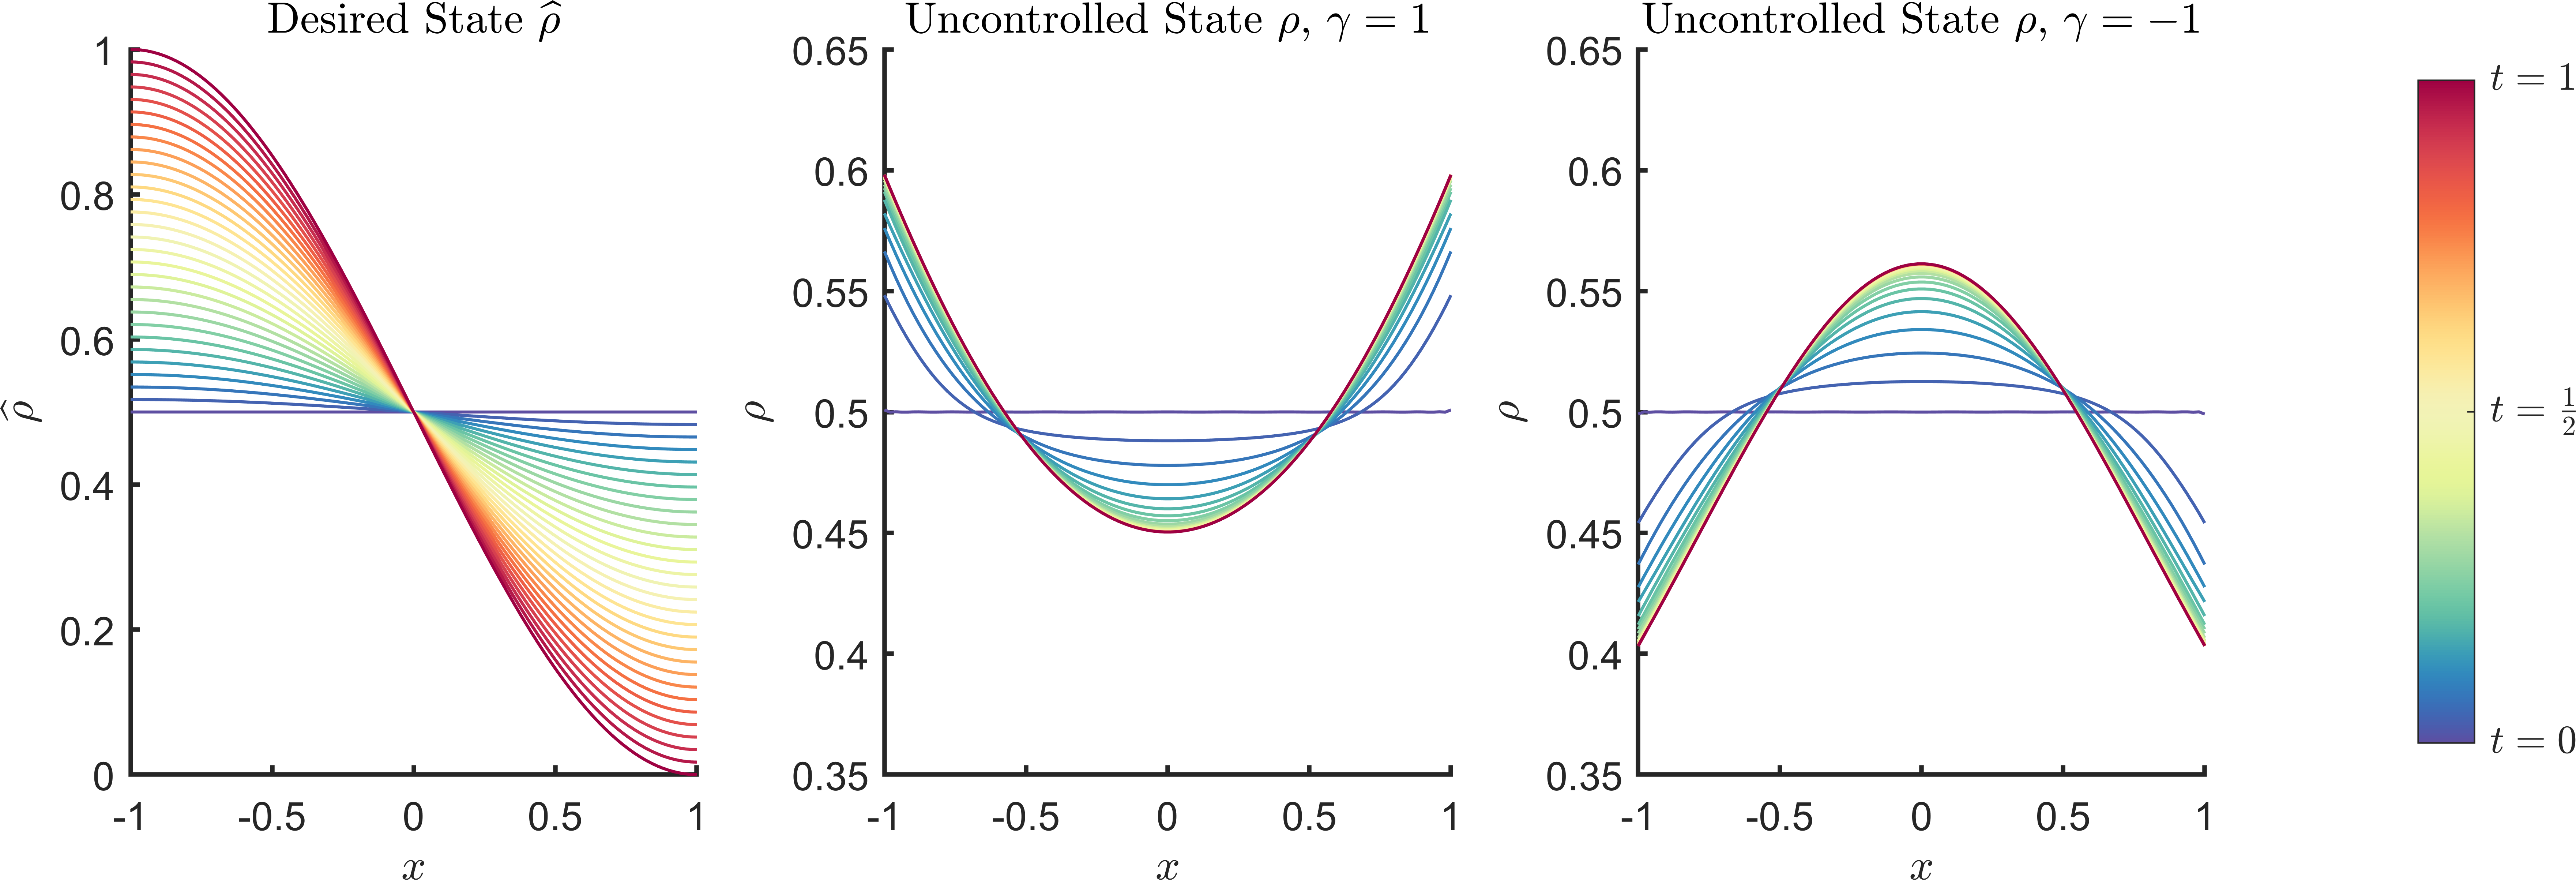
\includegraphics[scale=0.05]{Figure1.png}
	\caption{Example 1, desired state $\widehat \rho$ and uncontrolled state $\rho$ at $\gamma =1$ and $\gamma =-1$}
	\label{Ex12DN1}
\end{figure}
\begin{figure}[h]
	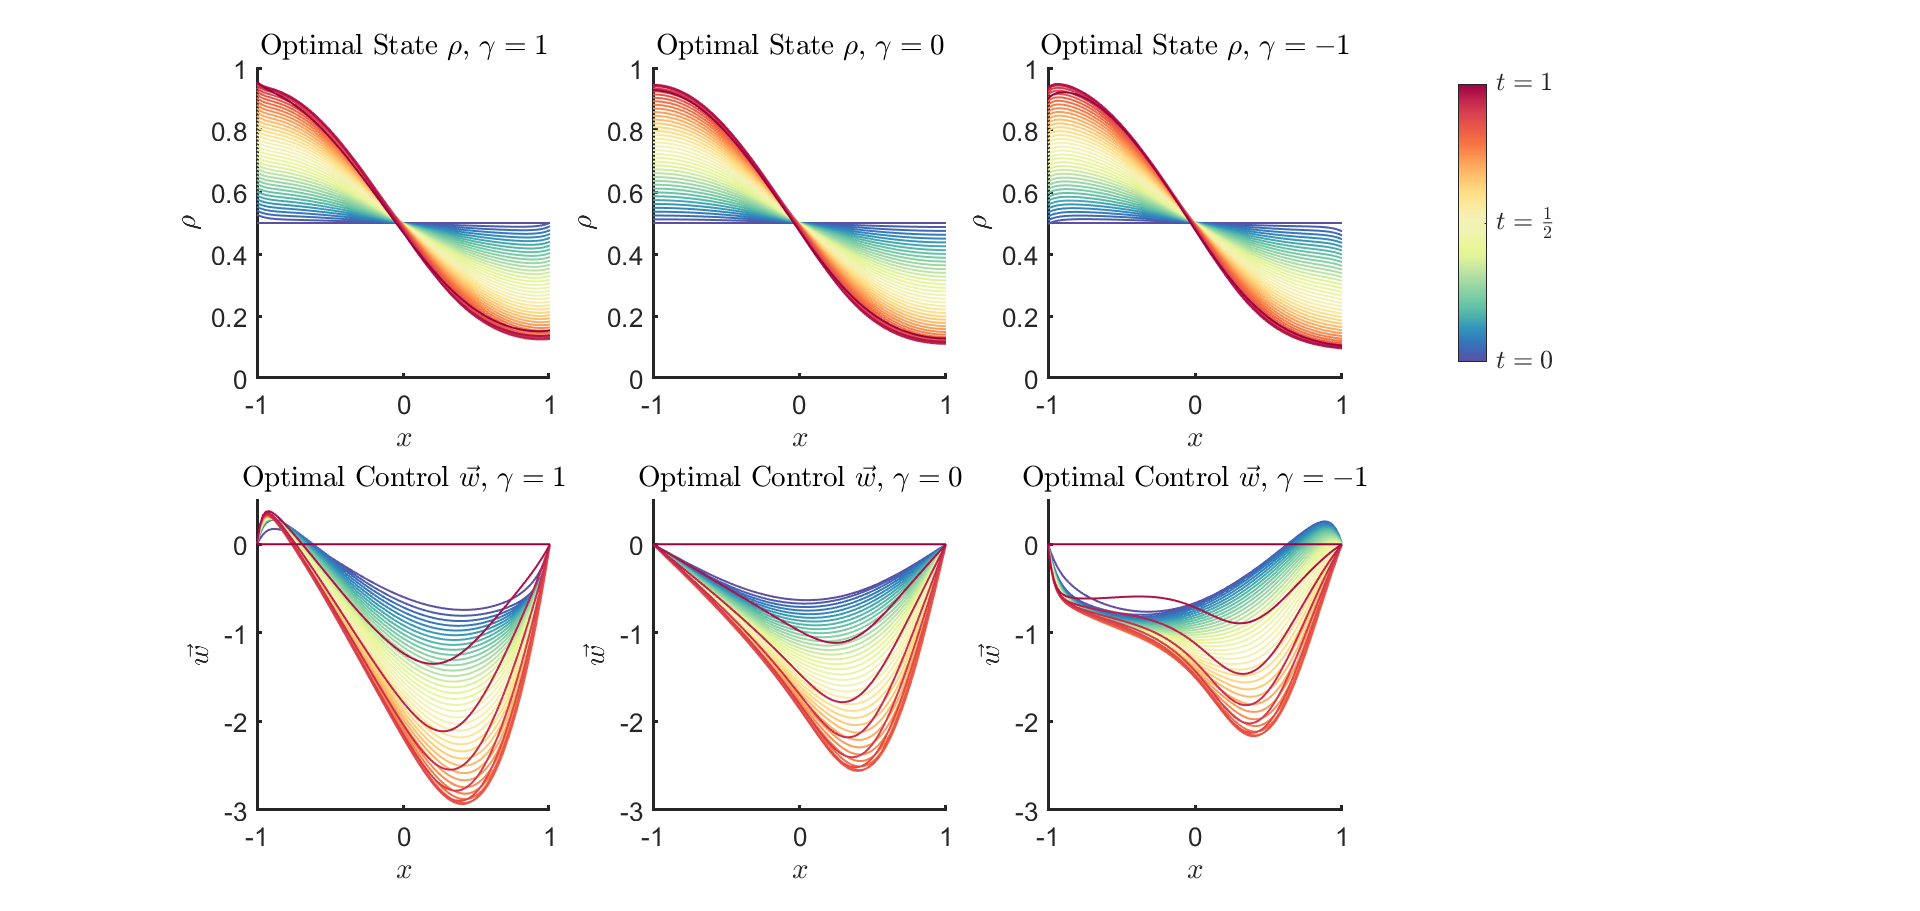
\includegraphics[scale=0.05]{Figure2.png}
	\caption{Example 1, optimal state $\rho$ and the corresponding optimal control $\vec{w}$ for $\gamma = 1,0,-1$, $\beta = 10^{-3}$.}
	\label{Ex12DN2}
\end{figure}

\begin{table}
\begin{tabular}{ | c | c || c | c | c | c ||}
\hline
\multicolumn{2}{|c||}{}& $\beta = 10^{-3}$ & $\beta = 10^{-1}$ & $\beta = 10^{1}$ & $\beta = 10^{3}$  \\
\hline
\hline
 & $\mathcal{J}_{uc}$ & $\numprint{0.0438}$ & $\numprint{0.0438}$ & $\numprint{0.0438}$ & $\numprint{0.0438}$ \\
$\kappa= \numprint{-1}$  & $\mathcal{J}_c$ & $\numprint{0.0011}$ & $\numprint{0.0267}$ & $\numprint{0.0435}$ & $\numprint{0.0438}$ \\
& \texttt{Iter} & $\numprint{670}$ & $\numprint{650}$ & $\numprint{449}$ & $\numprint{1}$ \\
\hline
 & $\mathcal{J}_{uc}$ & $\numprint{0.0417}$ & $\numprint{0.0417}$ & $\numprint{0.0417}$ & $\numprint{0.0417}$ \\
$\kappa= \numprint{0}$  & $\mathcal{J}_c$ & $\numprint{0.0014}$ & $\numprint{0.0283}$ & $\numprint{0.0415}$ & $\numprint{0.0417}$ \\
& \texttt{Iter} & $\numprint{665}$ & $\numprint{656}$ & $\numprint{434}$ & $\numprint{1}$ \\
\hline
 & $\mathcal{J}_{uc}$ & $\numprint{0.0434}$ & $\numprint{0.0434}$ & $\numprint{0.0434}$ & $\numprint{0.0434}$ \\
$\kappa= \numprint{1}$  & $\mathcal{J}_c$ & $\numprint{0.0020}$ & $\numprint{0.0322}$ & $\numprint{0.0432}$ & $\numprint{0.0434}$ \\
& \texttt{Iter} & $\numprint{654}$ & $\numprint{682}$ & $\numprint{422}$ & $\numprint{1}$ \\
\hline
\end{tabular}
\caption{Example 1: Uncontrolled cost $\mathcal{J}_{uc}$, optimal control cost $\mathcal{J}_{c}$, and number of iterations \emph{\texttt{Iter}}, for a range of $\kappa$ and $\beta$ values.}
\label{TabS5:Prob1}
\end{table} %\label{TabS5:Prob1}


\subsubsection{Neumann boundary conditions, Example 2} 
The chosen inputs for Example 2 are:
\begin{align*}
&\widehat \rho = \bigg(\frac{1}{2}\cos(\pi y) + \frac{1}{2}\bigg)(1-t) + t\bigg(-\frac{1}{2}\cos(2 \pi y) + \frac{1}{2}\bigg),\\
&\rho_{0} = \frac{1}{2}\cos(\pi y) + \frac{1}{2},\ \
\adj_{T} = 0,\ \
\vec{w} = \vec{0},\ \
f =0,\ \
V_{ext} =0.
\end{align*}
In Table \ref{TabS5:Prob2} the results for Example 2 are displayed. These are comparable with the results for Example 1, in the effect of $\beta$ and the number of iterations. In all three configurations of the interaction term, the control is focussed on transporting the mass from the middle of the domain onto two piles centred at $x=-0.5$ and $x=0.5$. In Figure \ref{Ex22DN1}, the desired state $\widehat \rho$, the optimal state $\rho$ and the optimal control $\vec{w}$ are displayed for $\beta = 10^{-3}$ and $\gamma = 1$, and compared to Example 3 below. Here, the number of points is chosen to be $N=40$ and $n=30$ (instead of $N=30$ and $n=20$), due to the steep gradients of the desired state.
\begin{figure}[h]
	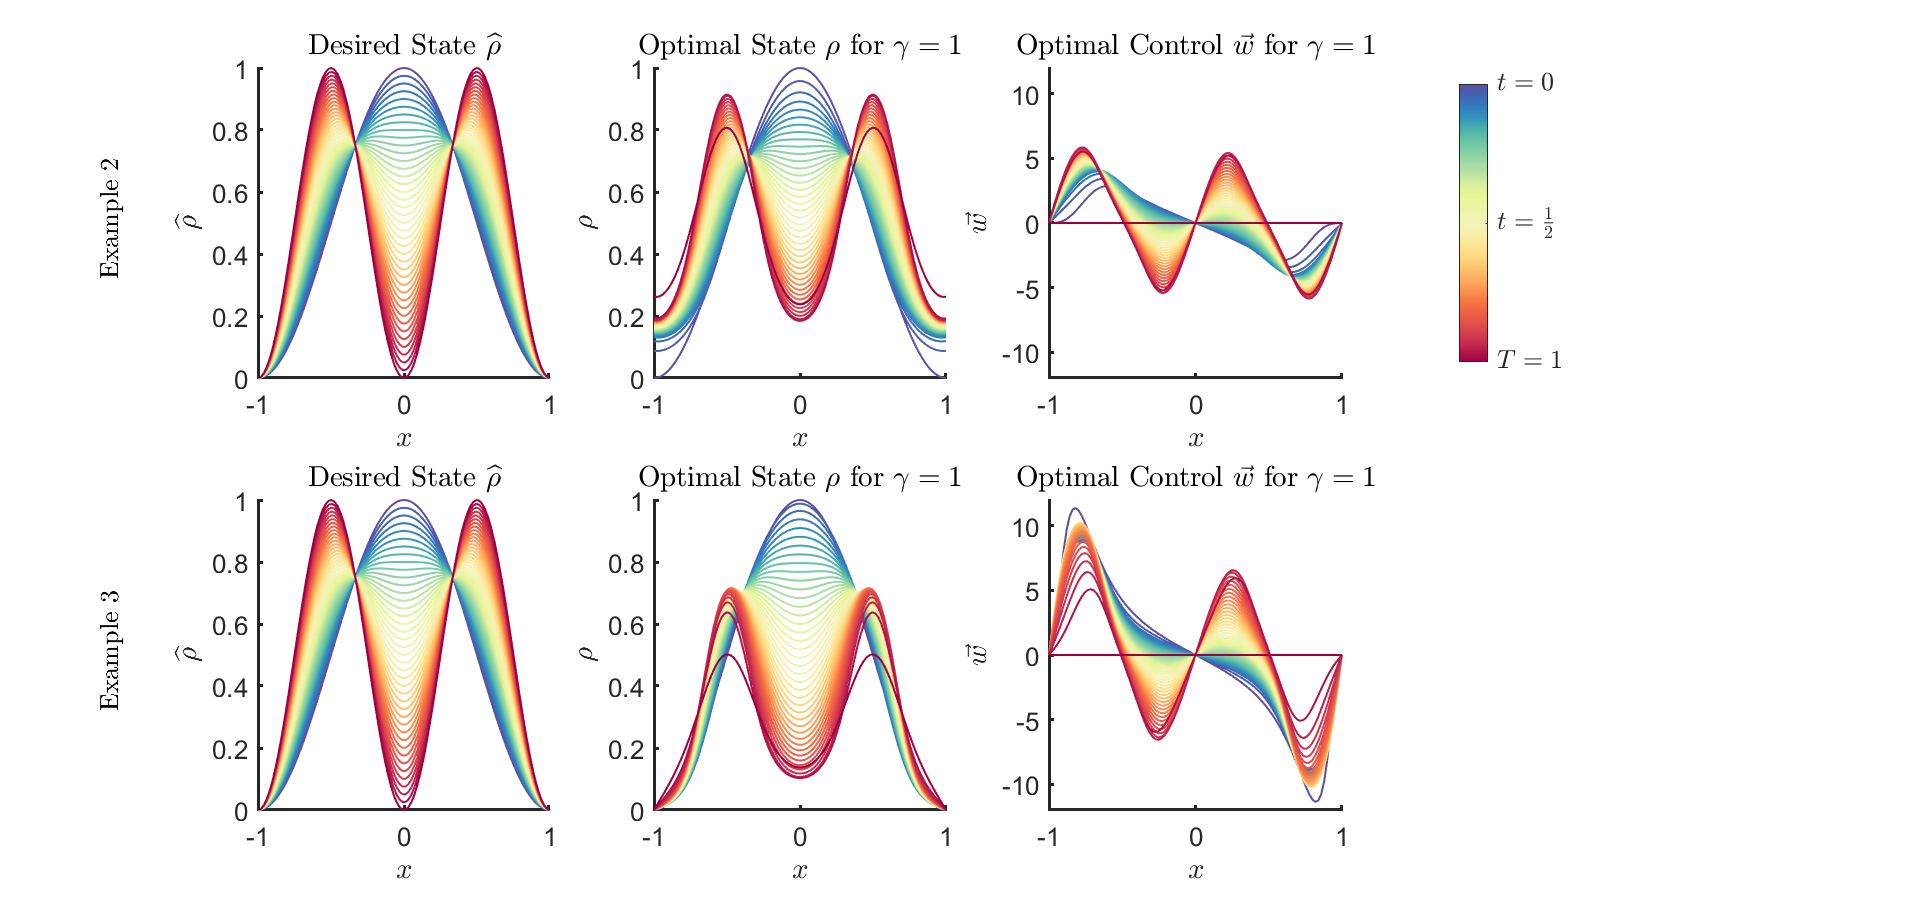
\includegraphics[scale=0.05]{Figure3.png}
	\caption{Example 2/ Example 3, desired state $\widehat \rho$, optimal state $\rho$ and corresponding optimal control $\vec{w}$, $\beta = 10^{-3}$, $\gamma = 1$.}
	\label{Ex22DN1}
\end{figure}

\begin{table}
\begin{tabular}{ | c | c || c | c | c | c ||}
\hline
\multicolumn{2}{|c||}{}& $\beta = 10^{-3}$ & $\beta = 10^{-1}$ & $\beta = 10^{1}$ & $\beta = 10^{3}$  \\
\hline
\hline
 & $\mathcal{J}_{uc}$ & $\numprint{0.0536}$ & $\numprint{0.0536}$ & $\numprint{0.0536}$ & $\numprint{0.0536}$ \\
$\kappa= \numprint{-1}$  & $\mathcal{J}_c$ & $\numprint{0.0096}$ & $\numprint{0.0492}$ & $\numprint{0.0535}$ & $\numprint{0.0536}$ \\
& \texttt{Iter} & $\numprint{715}$ & $\numprint{767}$ & $\numprint{367}$ & $\numprint{1}$ \\
\hline
 & $\mathcal{J}_{uc}$ & $\numprint{0.0669}$ & $\numprint{0.0669}$ & $\numprint{0.0669}$ & $\numprint{0.0669}$ \\
$\kappa= \numprint{0}$  & $\mathcal{J}_c$ & $\numprint{0.0109}$ & $\numprint{0.0603}$ & $\numprint{0.0668}$ & $\numprint{0.0669}$ \\
& \texttt{Iter} & $\numprint{714}$ & $\numprint{770}$ & $\numprint{390}$ & $\numprint{1}$ \\
\hline
 & $\mathcal{J}_{uc}$ & $\numprint{0.0839}$ & $\numprint{0.0839}$ & $\numprint{0.0839}$ & $\numprint{0.0839}$ \\
$\kappa= \numprint{1}$  & $\mathcal{J}_c$ & $\numprint{0.0125}$ & $\numprint{0.0748}$ & $\numprint{0.0838}$ & $\numprint{0.0839}$ \\
& \texttt{Iter} & $\numprint{713}$ & $\numprint{773}$ & $\numprint{403}$ & $\numprint{1}$ \\
\hline
\end{tabular}
\caption{Example 2: Cost when $\vec{w}=\vec{0}$, optimal control cost, and iterations required, for a range of $\kappa$, $\beta$.}
\label{TabS5:Prob2}
\end{table} %\label{TabS5:Prob2a}


\subsubsection{Dirichlet boundary conditions, Example 3} 
The inputs for this example are:
\begin{align*}
&\widehat \rho = \bigg(\frac{1}{2}\cos(\pi y) + \frac{1}{2}\bigg)(1-t) + t\bigg(-\frac{1}{2}\cos(2 \pi y) + \frac{1}{2}\bigg),\\
&\rho_{0} = \frac{1}{2}\cos(\pi y) + \frac{1}{2},\ \
\adj_{T} = 0,\ \
\vec{w} = \vec{0},\ \
f =0,\ \
V_{ext} =0.
\end{align*}
Table \ref{TabS5:Prob3} presents the results for this example, for a range of $\beta$ values and different interaction strengths. The observations are in line with those in Example 1 and 2. In particular, $ \widehat \rho$ and $\rho_0$ coincide with those of the problem with Neumann boundary conditions in Example 2. A comparison between the two examples is illustrated in Figure \ref{Ex22DN1}. Both the optimal state $\rho$ and the optimal control are qualitatively different when considering Dirichlet boundary conditions over Neumann conditions. The numerical result for this example was achieved with $N=40$ and $n = 30$, rather than with $N=30$ and $n=20$. This indicates that the Dirichlet boundary conditions are harder to apply in this problem, due to the steep shape of the desired state. This steepness is somewhat less impactful in Example 2, where the desired state is not closely matched by the optimal state at the boundaries. In Example 3, while the optimal state matches the desired state perfectly at the boundary, the peaks of the desired state are matched less closely. In Figure \ref{Ex22DN1}, this can be confirmed by considering the control plots. The optimal control for Example 3 is larger than for Example 2, specifically between the boundaries of the domain and the peaks of the desired state, indicating difficulties in this region.
\begin{table}
\begin{tabular}{ ||c|| c | c | c | c | c ||}
\hline
& & $\beta = 10^{-3}$ & $\beta = 10^{-1}$ & $\beta = 10^{1}$ & $\beta = 10^{3}$  \\
\hline
 & $J_{uc}$ & $\numprint{1.4165e-1}$ & $\numprint{1.4165e-1}$ & $\numprint{1.4165e-1}$ & $\numprint{1.4165e-1}$ \\
$\gamma= \numprint{-1}$  & $J_c$ & $\numprint{3.5594e-2}$ & $\numprint{1.3270e-1}$ & $\numprint{1.4155e-1}$ & $\numprint{1.4165e-1}$ \\
& $Iter.$ & $\numprint{944}$ & $\numprint{816}$ & $\numprint{437}$ & $\numprint{1}$ \\
\hline
 & $J_{uc}$ & $\numprint{1.5452e-1}$ & $\numprint{1.5452e-1}$ & $\numprint{1.5452e-1}$ & $\numprint{1.5452e-1}$ \\
$\gamma= \numprint{0}$  & $J_c$ & $\numprint{3.8023e-2}$ & $\numprint{1.4549e-1}$ & $\numprint{1.5442e-1}$ & $\numprint{1.5452e-1}$ \\
& $Iter.$ & $\numprint{940}$ & $\numprint{825}$ & $\numprint{440}$ & $\numprint{1}$ \\
\hline
 & $J_{uc}$ & $\numprint{1.6610e-1}$ & $\numprint{1.6610e-1}$ & $\numprint{1.6610e-1}$ & $\numprint{1.6610e-1}$ \\
$\gamma= \numprint{1}$  & $J_c$ & $\numprint{4.1143e-2}$ & $\numprint{1.5751e-1}$ & $\numprint{1.6601e-1}$ & $\numprint{1.6610e-1}$ \\
& $Iter.$ & $\numprint{932}$ & $\numprint{827}$ & $\numprint{440}$ & $\numprint{1}$ \\
\hline
\end{tabular}
\caption{Problem 3 ($n = 30,N = 40$)}
\label{TabS5:Prob3}
\end{table} %\label{TabS5:Prob3}


%\subsubsection{Neumann boundary conditions, Symmetric Example 1}
%Consider the following symmetric setup:
%\begin{align*}
%\widehat \rho &= \frac{1}{2}(1-t) + t\frac{1}{4}(\cos(\pi y)+2),\\
%\rho_{0} &= \frac{1}{2},\  \ q_{T} = 0, \ \ \vec{w} = \vec{0}, \ \  f =0, \ \ V_{ext} =0.
%\end{align*}
%Table \ref{TabNFlowAddEx1} summarizes the results for this example.The attractive interaction term causes $\rho$ to move towards the centre of the domain. Since $\widehat \rho$ is also centred in the domain, $J_{uc}$ is small for $\gamma =-1$ in comparison to the problems with $\gamma =0$ and $\gamma =1$. This example illustrates that the particle interaction term can have a significant impact on the optimization problem considered. 
%
%
%
%
%\subsubsection{Neumann boundary conditions, Symmetric Example 2}
%Consider the following symmetric setup, which is the opposite of the first symmetric example:
%\begin{align*}
%\widehat \rho &= \frac{1}{2}(1-t) + t\frac{1}{4}(-\cos(\pi y)+2),\\
%\rho_{0} &= \frac{1}{2},\ \
%q_{T} = 0,\ \
%\vec{w} = \vec{0},\ \
%f =0,\ \
%V_{ext} =0.
%\end{align*}
%This example can be compared to the Symmetric Example 1. Here, the desired state is having $\rho$ clustered at both boundaries, which is similar to the effect of the repulsive interaction term $\gamma = 1$. Therefore, for this choice of interaction term, the value of the cost functional $J_{uc}$ is smaller than the one for $\gamma = 0$ and $\gamma = -1$. This is the opposite to the observation made in the Symmetric Example 1, which is to be expected, given the two choices of desired state.


\subsection{Linear control problems with an additional nonlocal integral term}
In this section, examples of solving Problem \eqref{AdvDiff_Linear} with both 'no-flux type' boundary conditions \eqref{NoFlux_Linear} and Dirichlet boundary conditions \eqref{Dirichlet}.
\subsubsection{Dirichlet boundary conditions, Example 4}
The inputs for this example are:
\begin{align*}
&\widehat \rho = (1 - t)\bigg(\frac{1}{2}\cos(\pi y) + \frac{1}{2}\bigg)  + t\bigg(-\frac{1}{2}\cos(\pi y) + \frac{1}{2}\bigg),\\
&\rho_{0} = \frac{1}{2}\cos(\pi y) + \frac{1}{2},\ \
\adj_{T} = 0,\ \
{w} = 0,\ \
f =0, \ \
V_{ext} =\frac{1}{2}\left((x + 0.3)^2 - 0.2\right)\left((x-0.4)^2 - 0.3\right).
\end{align*}
In Table \ref{TabS5:Prob4} the results for Example 4 for a range of parameter values can be found. The results are qualitatively similar to the previous examples, but the control is applied linearly in this example. Note that here $\lambda = 0.005$, since $V_{{ext}}$ causes the numerical computations to be more challenging.
\begin{table}
\begin{tabular}{ | c | c || c | c | c | c ||}
\hline
\multicolumn{2}{|c||}{}& $\beta = 10^{-3}$ & $\beta = 10^{-1}$ & $\beta = 10^{1}$ & $\beta = 10^{3}$  \\
\hline
\hline
 & $\mathcal{J}_{uc}$ & $\numprint{0.1394}$ & $\numprint{0.1394}$ & $\numprint{0.1394}$ & $\numprint{0.1394}$ \\
$\kappa= \numprint{-1}$  & $\mathcal{J}_c$ & $\numprint{0.0183}$ & $\numprint{0.0862}$ & $\numprint{0.1384}$ & $\numprint{0.1394}$ \\
& \texttt{Iter} & $\numprint{1575}$ & $\numprint{1486}$ & $\numprint{1026}$ & $\numprint{117}$ \\
\hline
 & $\mathcal{J}_{uc}$ & $\numprint{0.1526}$ & $\numprint{0.1526}$ & $\numprint{0.1526}$ & $\numprint{0.1526}$ \\
$\kappa= \numprint{0}$  & $\mathcal{J}_c$ & $\numprint{0.0183}$ & $\numprint{0.0983}$ & $\numprint{0.1516}$ & $\numprint{0.1526}$ \\
& \texttt{Iter} & $\numprint{1582}$ & $\numprint{1474}$ & $\numprint{1023}$ & $\numprint{113}$ \\
\hline
 & $\mathcal{J}_{uc}$ & $\numprint{0.1645}$ & $\numprint{0.1645}$ & $\numprint{0.1645}$ & $\numprint{0.1645}$ \\
$\kappa= \numprint{1}$  & $\mathcal{J}_c$ & $\numprint{0.0189}$ & $\numprint{0.1103}$ & $\numprint{0.1635}$ & $\numprint{0.1645}$ \\
& \texttt{Iter} & $\numprint{1589}$ & $\numprint{1465}$ & $\numprint{1022}$ & $\numprint{112}$ \\
\hline
\end{tabular}
\caption{Example 4: Uncontrolled cost $\mathcal{J}_{uc}$, optimal cost $\mathcal{J}_{c}$, and number of iterations, for a range of $\kappa$ and $\beta$ values.}
\label{TabS5:Prob4}
\end{table} %\label{TabS5:Prob4}




\subsubsection{Neumann boundary conditions, Example 5}
The inputs for this example are:
\begin{align*}
&\widehat \rho = \frac{1}{2}(1-t) + t\frac{1}{2}(-\cos(\pi y) + 1),\\
&\rho_{0} = \frac{1}{2},\ \
\adj_{T} = 0,\ \
{w} = 0,\ \
f =0,\ \
V_{ext} =0.
\end{align*}
Table \ref{TabS5:Prob5} shows the results for Example 5. Note that for this example, when $\beta = 10^{-3}$, the mixing parameter $\lambda$ had to be set to $0.001$, to guarantee stable convergence of the method (why? explanation needed?).
Again, the only qualitative difference to interpreting the results is that the control is applied linearly.
\begin{table}
\begin{tabular}{ ||c|| c | c | c | c | c ||}
\hline
& & $\beta = 10^{-3}$ & $\beta = 10^{-1}$ & $\beta = 10^{1}$ & $\beta = 10^{3}$  \\
\hline
 & $J_{uc}$ & $\numprint{6.0640e-2}$ & $\numprint{6.0640e-2}$ & $\numprint{6.0640e-2}$ & $\numprint{6.0640e-2}$ \\
$\gamma= \numprint{-1}$  & $J_c$ & $\numprint{6.0180e-3}$ & $\numprint{5.5365e-2}$ & $\numprint{6.0592e-2}$ & $\numprint{6.0640e-2}$ \\
& $Iter.$ & $\numprint{7320}$ & $\numprint{7712}$ & $\numprint{3888}$ & $\numprint{1}$ \\
\hline
 & $J_{uc}$ & $\numprint{4.1667e-2}$ & $\numprint{4.1667e-2}$ & $\numprint{4.1667e-2}$ & $\numprint{4.1667e-2}$ \\
$\gamma= \numprint{0}$  & $J_c$ & $\numprint{4.5414e-3}$ & $\numprint{3.8334e-2}$ & $\numprint{4.1632e-2}$ & $\numprint{4.1667e-2}$ \\
& $Iter.$ & $\numprint{7271}$ & $\numprint{7614}$ & $\numprint{3643}$ & $\numprint{1}$ \\
\hline
 & $J_{uc}$ & $\numprint{2.8551e-2}$ & $\numprint{2.8551e-2}$ & $\numprint{2.8551e-2}$ & $\numprint{2.8551e-2}$ \\
$\gamma= \numprint{1}$  & $J_c$ & $\numprint{3.5942e-3}$ & $\numprint{2.6480e-2}$ & $\numprint{2.8529e-2}$ & $\numprint{2.8551e-2}$ \\
& $Iter.$ & $\numprint{7249}$ & $\numprint{7482}$ & $\numprint{3410}$ & $\numprint{1}$ \\
\hline
\end{tabular}
\caption{Problem 5}
\label{TabS5:Prob5}
\end{table} %\label{TabS5:Prob5}


\subsection{Nonlinear control problems with an additional nonlocal integral term in 2D}
In this section, two-dimensional examples are considered, to illustrate the fact that the application of the method differs very little from the one dimensional setting. The main difference is that in nonlinear control problems the control is a two-dimensional vector field. Furthermore, the number of spatial points increases from $N$ to $N_1\times N_2$, which makes computations much more costly. Compensating for this increased cost is one of the motivations to develop fast optimization solvers, such as the fixed point method introduced in Section \ref{sec:Method_Solver}.
\subsubsection{Neumann boundary conditions, Example 1}	
We have the following set up:
\begin{align*}
&\widehat \rho = \frac{1}{4}(1-t) + t\bigg(\frac{1}{4}\sin \bigg(\frac{\pi}{2}(x_1 - 2)\bigg)\sin \bigg(\frac{\pi}{2}(x_2 - 2)\bigg) + \frac{1}{4}\bigg),\\
&\rho_0 = \frac{1}{4},\ \
q_{T} = 0,\ \
\vec{w} = \vec{0},\ \
f =0,\ \
V_{ext} =0.
\end{align*}
This example is the two dimensional version of Example 1 in Section \ref{sec:Examples1d}. The results for this example are displayed in Table \ref{TabS5:Prob12D}. In Figures \ref{rhoHat2dEx2} it can be observed that as in Example 1 in Section \ref{sec:Examples1d}, the uncontrolled state forms a cluster in the centre of the domain, due to the attractive interactions. Figure \ref{rhoOpt2dEx2} shows the optimal state and control for different time points, for $\beta = 10^{-3}$ and $\gamma = -1$. Here, the control through a vector field illustrates why nonlinear control is called 'flow control'. 

\begin{table}
\begin{tabular}{ ||c|| c | c | c | c | c ||}
\hline
& & $\beta = 10^{-3}$ & $\beta = 10^{-1}$ & $\beta = 10^{1}$ & $\beta = 10^{3}$  \\
\hline
 & $\mathcal J_{\vec w = \vec 0}$ & $0.0113$ & $0.0113$ & $0.0113$ & $0.0113$ \\
$\kappa= -1$  & $\mathcal J_{Opt}$ & $0.0013$ & $0.0104$ & $0.0113$ & $0.0113$ \\
& $\text{Iterations}$ & $676$ & $700$ & $290$ & $1$ \\
\hline
\end{tabular}
\caption{Results for the test problem, with different $\beta$}
\label{TabS5:Prob12D}
\end{table} % \label{TabS5:Prob12D}

\begin{figure}[h]
	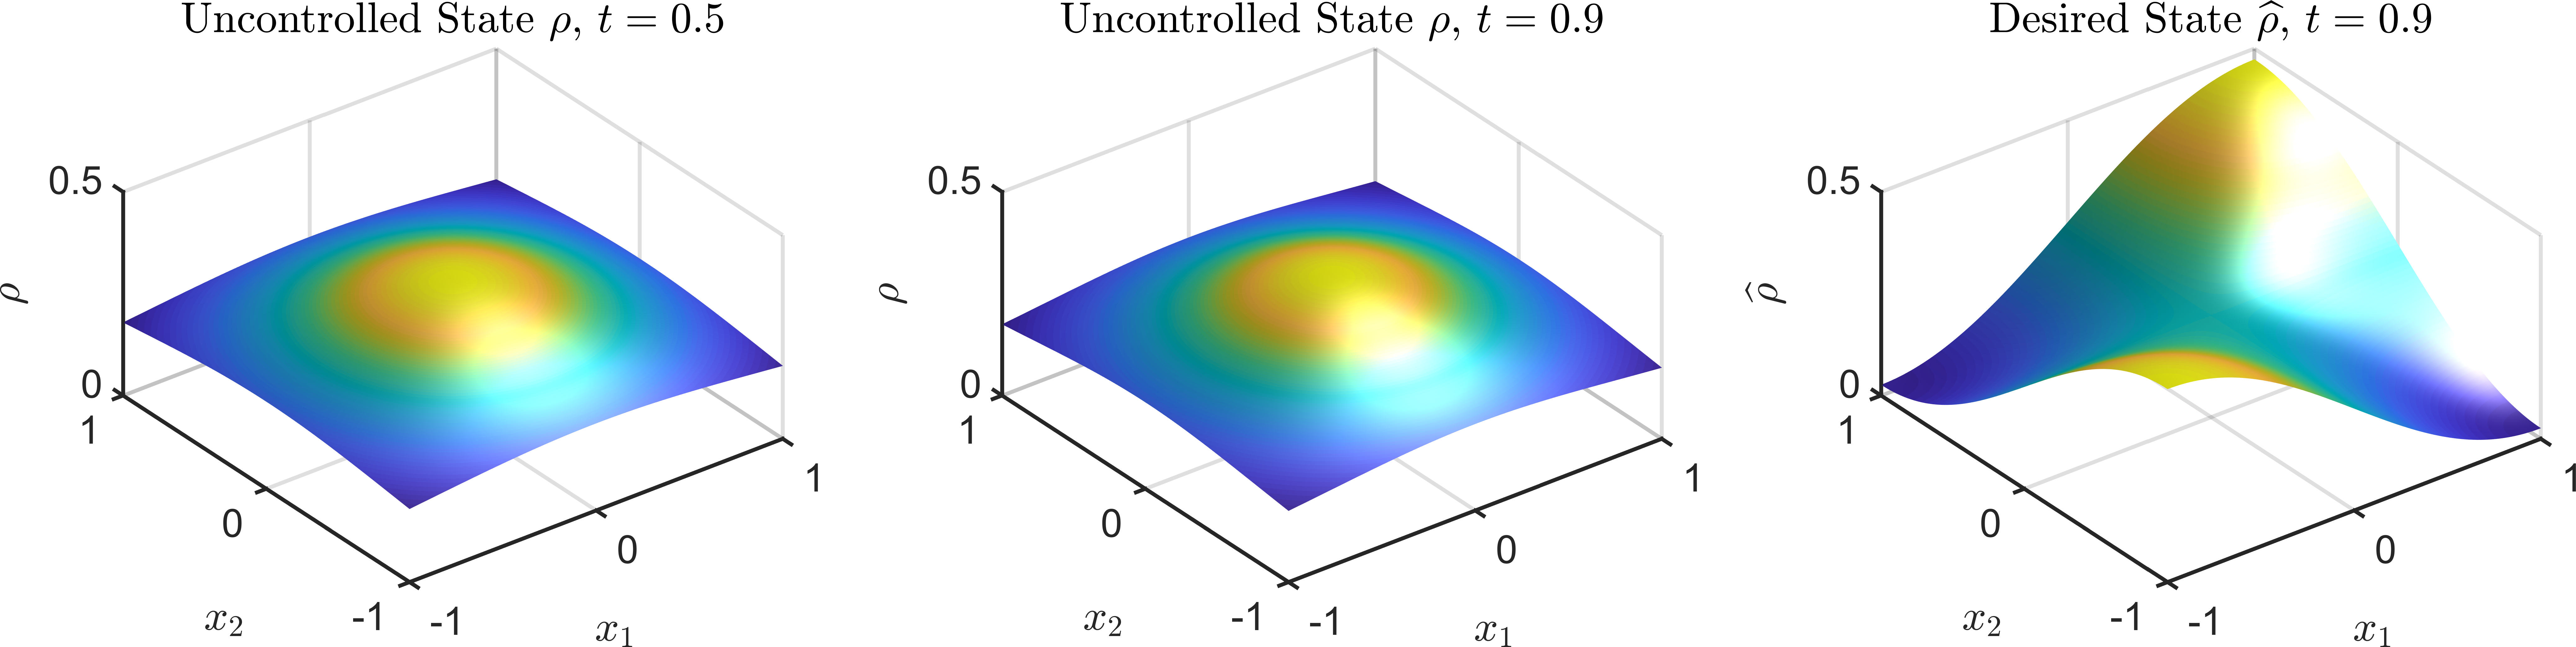
\includegraphics[scale=0.05]{Figure12D.png}
	\caption{2D Example 1, uncontrolled $\rho$ and $\widehat \rho$, $\beta = 10^{-3}$, $\gamma = -1$.}
	\label{rhoHat2dEx2}
\end{figure}
\begin{figure}[h]
	\includegraphics[scale=0.06]{Figure22D.png}
	\caption{2D Example 1, controlled $\rho$ and optimal control $\vec{w}$, $\beta = 10^{-3}$, $\gamma = -1$.}
	\label{rhoOpt2dEx2}
\end{figure}


\subsubsection{Neumann boundary conditions, Example 2}	
Here, we have:
\begin{align*}
&\widehat \rho = \frac{1}{4}(1-t) + t\frac{1}{0.9921}e^{-3((y_1+0.2)^2 + (y_2+0.2)^2))},\\
&\rho_0 = \frac{1}{4},\ \
q_{T} = 0,\ \
\vec{w} = \vec{0},\ \
f =0,\\
&V_{ext} =\left((x_1 + 0.3)^2 - 1\right)\left((x_1-0.4)^2 - 0.5\right)
\left((x_2 + 0.3)^2 - 1\right)\left((x_2-0.4)^2 - 0.5\right).
\end{align*}
The numerical results for this example are displayed in Table \ref{TabS5:Prob22D}. In figures \ref{rhoHat2dEx4} and \ref{rhoOpt2dEx4} the results are illustrated for $\beta = 10^{-3}$ and $\gamma = -1$. It can be observed very clearly that the control is driving the particle distribution to the desired state. It is noticeable that the control does not act uniformly around the peak of the desired state, but also acts strongly in the area between the location of the desired peak and the point $(-1,1)$. This is due to the external potential being steep in this area and more control is needed to reach the desired state than in other parts of the domain.

\begin{table}
\begin{tabular}{ | c | c || c | c | c | c ||}
\hline
\multicolumn{2}{|c||}{}& $\beta = 10^{-3}$ & $\beta = 10^{-1}$ & $\beta = 10^{1}$ & $\beta = 10^{3}$  \\
\hline
\hline
 & $\mathcal{J}_{uc}$ & $\numprint{0.0378}$ & $\numprint{0.0378}$ & $\numprint{0.0378}$ & $\numprint{0.0378}$ \\
$\kappa= \numprint{-1}$  & $\mathcal{J}_c$ & $\numprint{0.0017}$ & $\numprint{0.0312}$ & $\numprint{0.0377}$ & $\numprint{0.0378}$ \\
& \texttt{Iter} & $\numprint{691}$ & $\numprint{736}$ & $\numprint{347}$ & $\numprint{1}$ \\
\hline
 & $\mathcal{J}_{uc}$ & $\numprint{0.0478}$ & $\numprint{0.0478}$ & $\numprint{0.0478}$ & $\numprint{0.0478}$ \\
$\kappa= \numprint{0}$  & $\mathcal{J}_c$ & $\numprint{0.0064}$ & $\numprint{0.0450}$ & $\numprint{0.0478}$ & $\numprint{0.0478}$ \\
& \texttt{Iter} & $\numprint{718}$ & $\numprint{784}$ & $\numprint{343}$ & $\numprint{1}$ \\
\hline
 & $\mathcal{J}_{uc}$ & $\numprint{0.0526}$ & $\numprint{0.0526}$ & $\numprint{0.0526}$ & $\numprint{0.0526}$ \\
$\kappa= \numprint{1}$  & $\mathcal{J}_c$ & $\numprint{0.0137}$ & $\numprint{0.0514}$ & $\numprint{0.0526}$ & $\numprint{0.0526}$ \\
& \texttt{Iter} & $\numprint{735}$ & $\numprint{790}$ & $\numprint{338}$ & $\numprint{1}$ \\
\hline
\end{tabular}
\caption{2D Ex. 2: Uncontrolled cost $\mathcal{J}_{uc}$, optimal cost $\mathcal{J}_{c}$, and number of iterations, for a range of $\kappa$ and $\beta$ values.}
\label{TabS5:Prob22D}
\end{table} %\label{TabS5:Prob22D}

\begin{figure}[h]
	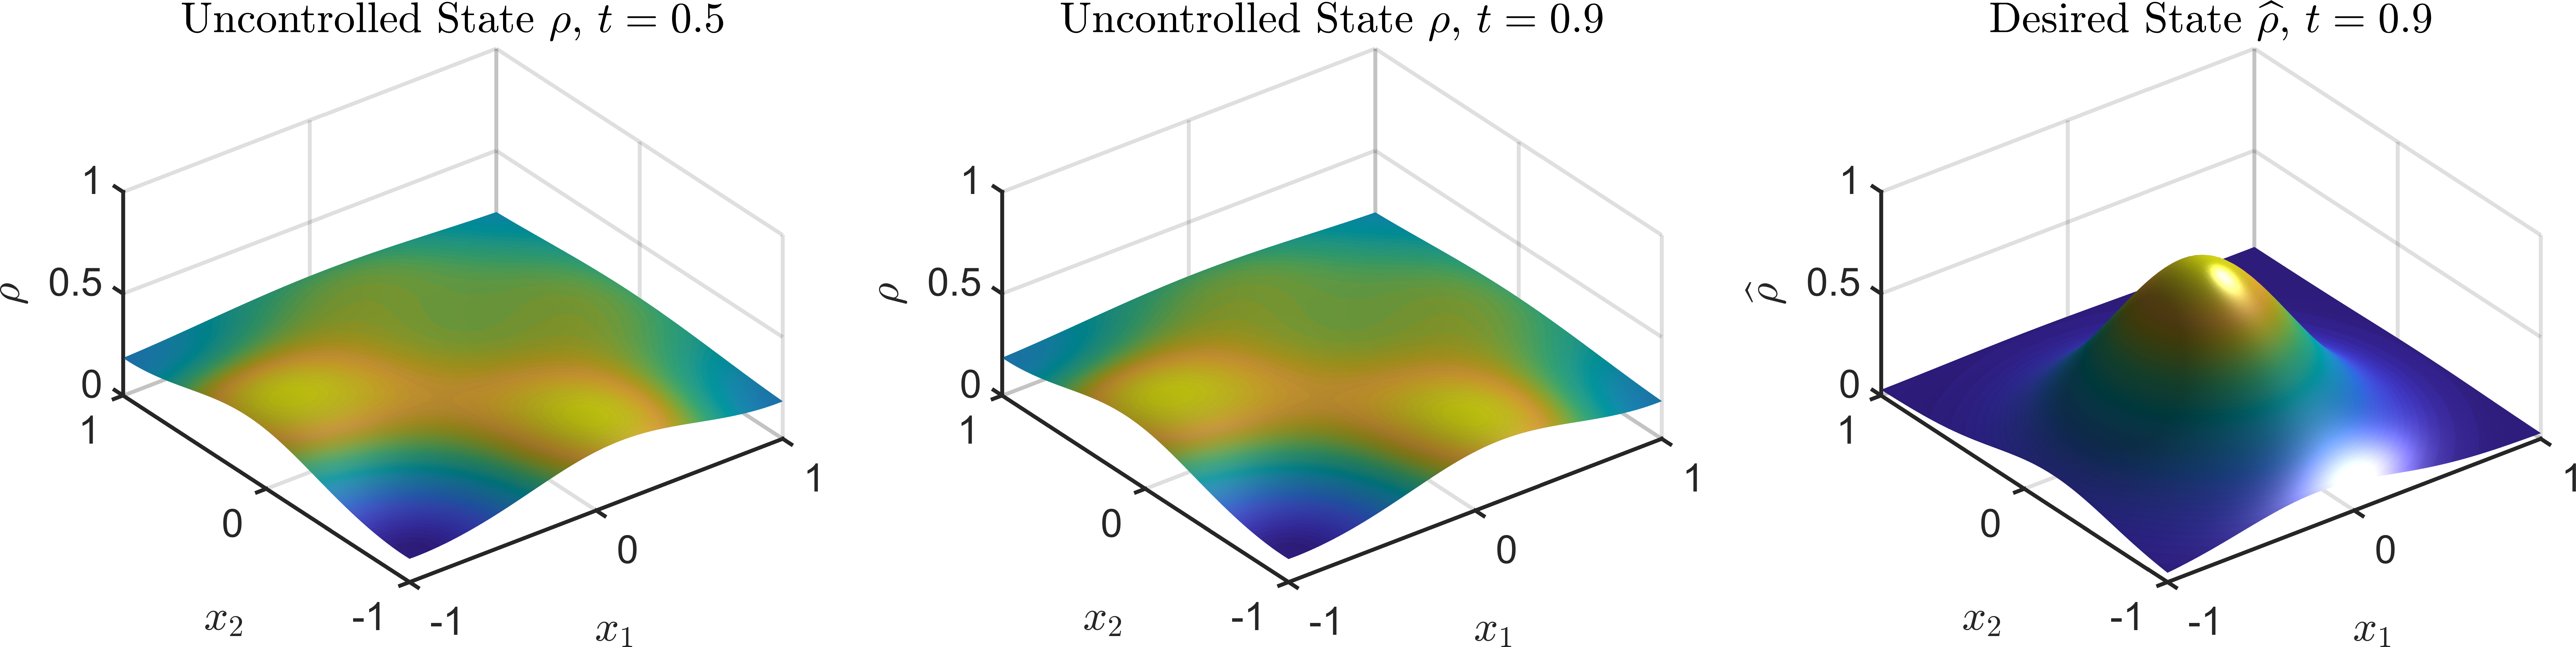
\includegraphics[scale=0.05]{Figure32D.png}
	\caption{2D Example 2: Uncontrolled $\rho$ and desired state $\widehat \rho$,  with $\beta = 10^{-3}$ and $\kappa = -1$. }
	\label{rhoHat2dEx4}
\end{figure}
\begin{figure}[h]
	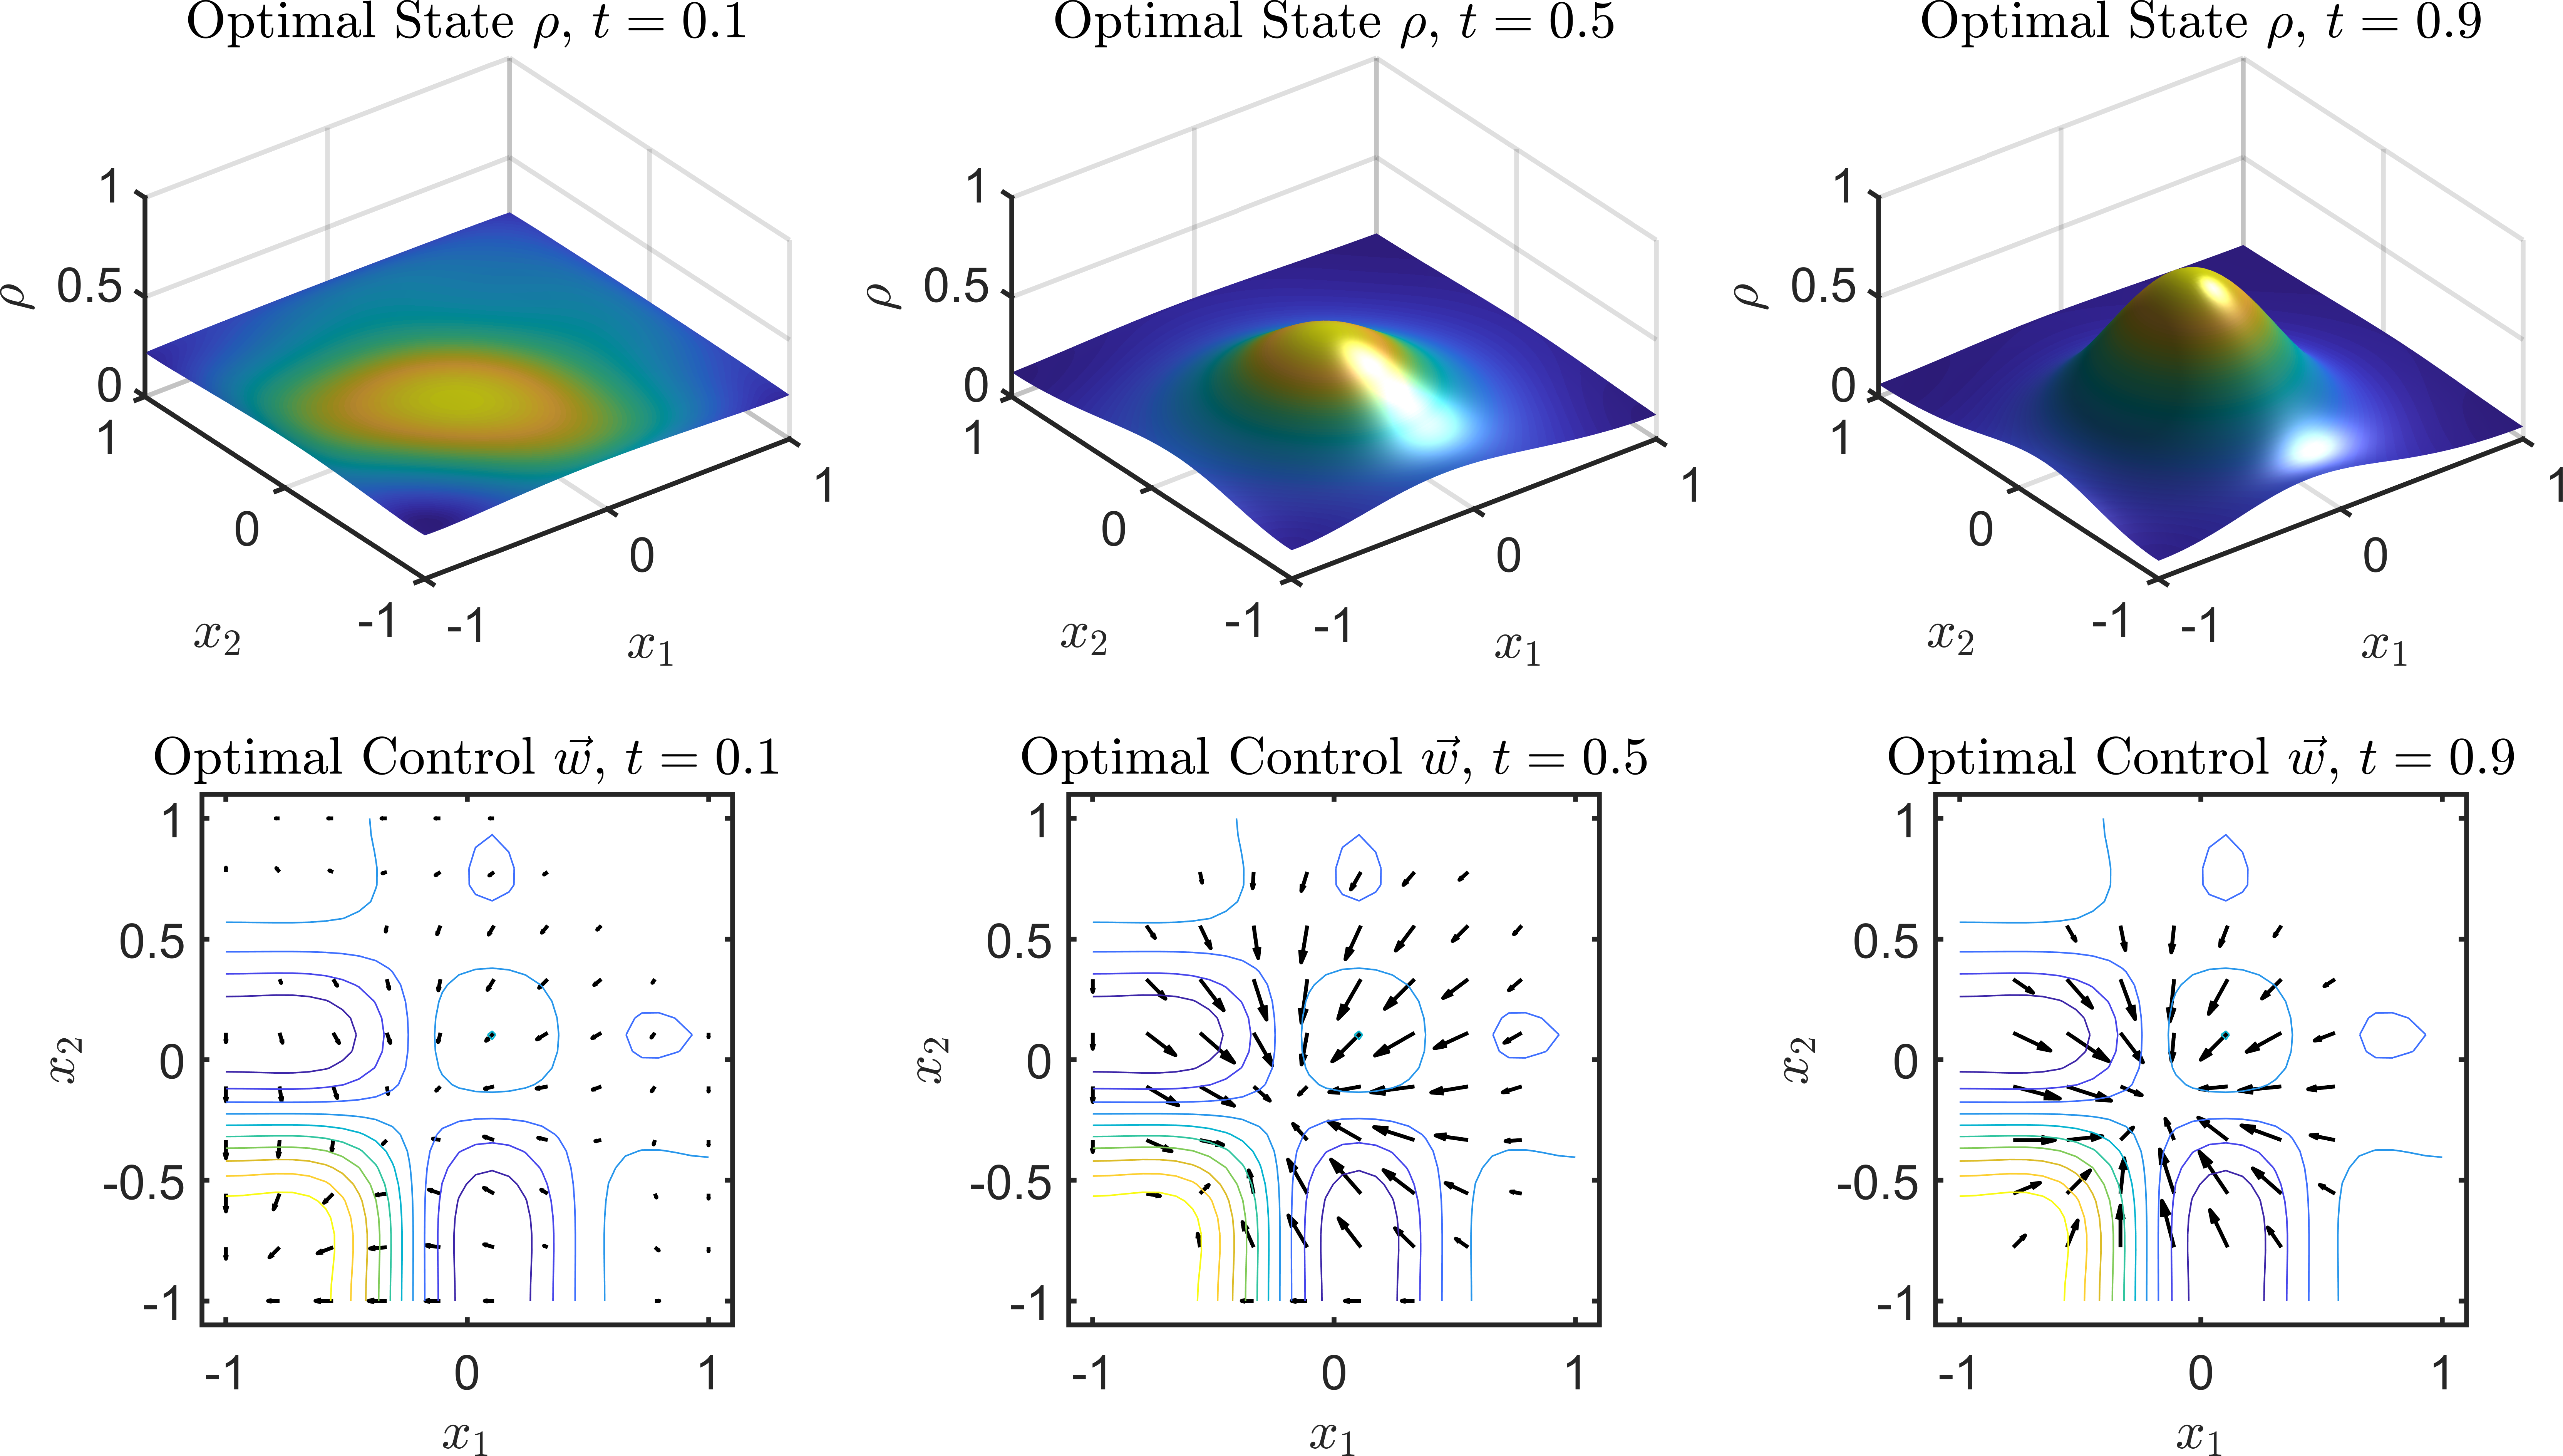
\includegraphics[scale=0.06]{Figure42D.png}
	\caption{2D Example 2: Optimal state $\rho$ and optimal control $\vec{w}$, with $\beta = 10^{-3}$ and $\kappa = -1$. A contour plot of the external potential $V^{\text{ext}}$ is superimposed on the control plots for reference.} 
	\label{rhoOpt2dEx4}
\end{figure}








	
	
	\section{Conclusion}
	During the past year, a fast and accurate optimization solver has been developed, which reliably solves various optimal control problems. In the course of the next year, this will be applied to different model problems, such as models with inertial effects. Furthermore, the numerical method is extended to be applied to different domains. At the present time, only rectangular domains are considered. However, in the following year, the optimal control problems will be solved on more complex domains, which are composed of quadrilateral and circular shapes. 
	Other possibilities to be considered are models including multiple species and different control types other than flow and source control.
	The main aim is to extend the model and the numerical method to industrial applications.
	

\section*{Year 3}	
	
	
	
	
	
	
	
	
	
	
	
	\pagebreak	
	\bibliography{GeneralBib}
	\bibliographystyle{unsrt}
	
	
\end{document}